\documentclass[journal]{new-aiaa}

\usepackage[utf8]{inputenc}
\usepackage{textcomp}
\usepackage{graphicx}
\usepackage{amsmath}
\usepackage[version=4]{mhchem}
\usepackage{siunitx}
\usepackage{longtable,tabularx}
\setlength\LTleft{0pt}
\usepackage{placeins}


\title{Hierarchical Aerodynamic Knowledge Transfer for Data-Efficient
Surface Pressure Prediction of Transonic Swept Wings}


% Replace the author, footnote, and affiliation placeholders before submission.
\author{Author Name\footnote{Position, Department, mailing address, and AIAA
Member Grade (if applicable); corresponding author: email address.}}
\affil{Institution, City, Province or State, Postal Code, Country}


\begin{document}

\maketitle


% Abstract intentionally left empty for later completion.
% \begin{abstract}
% \end{abstract}


% Nomenclature will be completed later.
% \section*{Nomenclature}

\noindent All coefficients, ratios, normalized coordinates, and model gates
are dimensionless unless units are stated.

{\renewcommand\arraystretch{1.0}
\noindent\begin{longtable*}{@{}l @{\quad=\quad} p{0.76\textwidth}@{}}
\multicolumn{2}{@{}l}{\textit{Roman symbols}}\\
$AR$                         & wing aspect ratio \\
$b$                          & wingspan, m \\
$c$                          & chord length, m \\
$C_D$                        & drag coefficient \\
$C_L$                        & lift coefficient \\
$C_{M_z}$                    & moment coefficient about the $z$ axis \\
$C_p$                        & pressure coefficient, $(p-p_\infty)/q_\infty$ \\
$C_p^{\mathrm{sec}}$         & sectional pressure baseline supplied by the knowledge model \\
$G(\eta,x)$                  & parameterized wing-surface geometry \\
$g_r,\ g_t$                  & spatial gates for the root- and tip-region corrections \\
$L_2$                        & Euclidean norm used to monitor iterative convergence \\
$M_\infty$                   & freestream Mach number \\
$N$                          & number of complete target-wing training samples \\
$N_c,\ N_s,\ N_n$            & chordwise, spanwise, and wall-normal grid-point counts \\
$N_x,\ N_\eta$               & numbers of chordwise and spanwise prediction points \\
$p$                          & local static pressure, Pa \\
$p_\infty$                   & freestream static pressure, Pa \\
$q_\infty$                   & freestream dynamic pressure, Pa \\
$Re_c$                       & Reynolds number based on chord length \\
$R_\theta$                   & target-domain three-dimensional pressure residual \\
$t/c$                        & thickness-to-chord ratio \\
$x/c$                        & normalized chordwise coordinate \\
$z$                          & spanwise coordinate, m \\
\\[-0.2em]
\multicolumn{2}{@{}l}{\textit{Greek symbols}}\\
$\alpha$                     & angle of attack, deg \\
$\Delta(\cdot)$              & difference relative to the stated reference solution \\
$\Delta C_{p,r}$             & root-region pressure correction \\
$\Delta C_{p,t}$             & tip-region pressure correction \\
$\eta$                       & normalized semispan coordinate, $z/(b/2)$ \\
$\lambda$                    & wing taper ratio \\
$\Lambda_{c/4}$              & quarter-chord sweep angle, deg \\
$\theta$                     & trainable model parameters \\
\\[-0.2em]
\multicolumn{2}{@{}l}{\textit{Subscripts and superscripts}}\\
$c$                          & quantity based on the chord length \\
$r$                          & root-region quantity \\
$t$                          & tip-region quantity \\
$\infty$                     & freestream quantity \\
$\mathrm{3D}$                & three-dimensional target quantity \\
$\mathrm{sec}$               & sectional-baseline quantity \\
\end{longtable*}}

% longtable increments the table counter even though nomenclature is unnumbered.
\addtocounter{table}{-1}




\begin{abstract}
High-fidelity three-dimensional (3-D) computational fluid dynamics (CFD) data are expensive to generate, limiting the training of deep-learning models for transonic finite-wing surface-pressure prediction. Lower-dimensional aerodynamic data provide transferable sectional information but cannot fully represent finite-span effects, particularly near the wing root and tip. To address this limitation, this study develops a hierarchical aerodynamic knowledge-transfer framework that separates sectional pressure responses from localized three-dimensional corrections. A baseline pressure model is trained on infinite-span swept-wing data, while root- and tip-correction models are developed using pressure differences between paired finite- and infinite-span CFD solutions. These knowledge models are transferred to the target wing to construct a three-dimensional pressure prior, which is subsequently refined through residual learning using limited target-domain CFD samples. With only 10 target-wing training samples, the proposed method reduces the surface-pressure root-mean-square error by 65.74\% relative to direct three-dimensional learning and achieves lower prediction error than the direct-learning model trained with 50 samples. Ablation studies further demonstrate the complementary contributions of root and tip corrections. In a downstream aerodynamic-coefficient regression task using 20 force-labeled wings, incorporating pressure distributions predicted by a separately trained model reduces the mean absolute errors in lift and drag coefficients by 70.1\% and 54.8\%, respectively, compared with direct regression. These results demonstrate that combining transferable sectional knowledge with localized finite-span corrections provides an effective aerodynamic prior, substantially improving the data efficiency of three-dimensional wing pressure prediction.
\end{abstract}


% ============================================================
% I. Introduction
% ============================================================

\section{Introduction}
\label{sec:introduction}

\lettrine{A}{ccurate} characterization of wing aerodynamics requires not only integrated force and moment coefficients but also the surface pressure distribution, which provides spatially resolved information on aerodynamic loading, shock-wave behavior, and other local flow features. Reynolds-averaged Navier--Stokes (RANS) computational fluid dynamics (CFD) remains one of the primary tools for obtaining such high-fidelity aerodynamic information. However, aerodynamic design typically requires repeated evaluations over variations in geometry and operating conditions, causing the computational cost of CFD to increase rapidly in multipoint analysis, parametric studies, and aerodynamic optimization. This issue becomes particularly pronounced for transonic wings, where shock waves, shock--boundary-layer interactions, and possible flow separation introduce strong nonlinearities into the aerodynamic response. Consequently, developing rapid predictive models that retain the spatial information of high-fidelity CFD while substantially reducing the evaluation cost has become an important topic in data-driven aerodynamics \cite{Brunton2020MLFluid}.

Deep learning provides an effective means of constructing aerodynamic surrogate models by learning nonlinear mappings between geometry, flow conditions, and distributed aerodynamic quantities. For two-dimensional airfoils, convolutional and encoder--decoder neural networks have been successfully used to predict pressure and velocity fields over previously unseen geometries \cite{Bhatnagar2019CNNFlow,Thuerey2020DeepRANS}. Subsequent studies have demonstrated accurate prediction of airfoil surface pressure distributions and transonic flow fields involving shock waves and flow separation \cite{Hui2020FastPressure,Duru2022TransonicFlow}. Compared with surrogate models that predict only integrated aerodynamic coefficients, distributed-field prediction preserves local aerodynamic information and therefore provides a more informative basis for load evaluation, flow-feature analysis, and aerodynamic design. More recently, data-driven models have also been extended to three-dimensional configurations, including aerodynamic surface-pressure prediction on general three-dimensional geometries and reduced-order prediction of transonic wing flow fields \cite{Shen2023General3D,Immordino2024TransonicDL}. These developments demonstrate the potential of deep learning for rapid three-dimensional aerodynamic prediction, while also exposing a fundamental difficulty: generating sufficiently diverse high-fidelity three-dimensional training data is considerably more expensive than generating corresponding two-dimensional data.

One possible route to reducing this data requirement is to exploit the physical relationship between lower-dimensional sectional aerodynamics and finite-wing flows. Classical sweep corrections and quasi-three-dimensional approaches seek to approximate three-dimensional wing aerodynamics through appropriately transformed two-dimensional or infinite-swept-wing solutions. In particular, 2.75D approaches incorporate sweep- and taper-related effects into sectional analyses and have been successfully employed for transonic wing analysis and design at a computational cost substantially lower than that of full three-dimensional optimization \cite{Zhao2016SupercriticalWing,Xu2022Improved275D}. A similar principle has recently been introduced into data-driven modeling. Li et al. transferred aerodynamic knowledge learned from two-dimensional supercritical airfoils to three-dimensional transonic swept wings \cite{Li2023AirfoilToWing}, while Yang et al. further embedded sweep theory into an airfoil-to-wing transfer-learning framework \cite{Yang2025PhysicsEmbeddedTransfer}. These studies indicate that lower-dimensional aerodynamic information contains transferable pressure characteristics and flow features that can provide useful priors for three-dimensional prediction.

Nevertheless, the relationship between sectional aerodynamics and a finite wing is inherently nonuniform along the span. Section-based or conical-flow approximations are most applicable where the local flow remains approximately quasi-two-dimensional, whereas their assumptions progressively deteriorate in regions dominated by finite-wing effects. In fact, the applicability of the 2.75D transformation has been reported to be limited in regions with strong three-dimensional effects, particularly near the wing root and wing tip \cite{Xu2022Improved275D}. Experimental investigations of finite transonic wings have likewise shown that sweep, spanwise flow, and tip-vortex effects can substantially modify the local flow relative to the corresponding two-dimensional configuration \cite{DAguanno2022FiniteWing}. Under transonic conditions, spanwise variations in shock location and strength further enhance this spatial nonuniformity. Consequently, a sectional pressure model may reproduce the dominant chordwise pressure characteristics over much of the wing while still exhibiting systematic local discrepancies in the root and tip regions. Accurately representing these regional three-dimensional effects is therefore essential if lower-dimensional aerodynamic knowledge is to be used as a reliable prior for full finite-wing pressure prediction.

The limited availability of three-dimensional training data provides a second challenge. Transfer learning and multifidelity learning have therefore been increasingly introduced into aerodynamic modeling to reuse information obtained from related configurations or lower-cost data. Multifidelity neural-network models have demonstrated that inexpensive aerodynamic data can be combined with a smaller number of high-fidelity samples to improve aerodynamic surrogate modeling \cite{Zhang2021MultifidelityDNN,Li2022Multifidelity,Leng2024VariableFidelity}. For flow-field prediction, Wang et al. employed transfer learning to improve airfoil-flow prediction when only a small target-domain dataset was available \cite{Wang2023DeepTransfer}. At the wing level, spatial dependencies learned from available pressure information have been transferred between spanwise sections \cite{Qu2022SpatialTransfer}, while transferable neural-network architectures have been used to reduce the number of samples required when extending aerodynamic models across swept-wing configurations \cite{Yang2024TransferableWing}. Physics-embedded airfoil-to-wing transfer further demonstrates that explicitly incorporating sectional aerodynamic knowledge can substantially reduce the amount of three-dimensional wing data required for model construction \cite{Yang2025PhysicsEmbeddedTransfer}. However, transferred knowledge remains effective only insofar as the source-domain representation captures the relevant physics of the target flow; discrepancies associated with finite-span and strongly three-dimensional local effects cannot generally be eliminated by transferring sectional information alone.

The existing literature therefore reveals a central tradeoff in small-sample finite-wing prediction. Lower-dimensional aerodynamic data are relatively inexpensive to generate and contain reusable information about the fundamental chordwise pressure response, but they cannot fully represent spatially localized three-dimensional effects. High-fidelity finite-wing data retain these effects directly, but obtaining sufficient samples to cover the combined geometry--condition space is computationally expensive. Thus, the key issue is not simply how to transfer two-dimensional knowledge to a three-dimensional model, but how to distinguish aerodynamic information that is broadly reusable from that associated with specific finite-wing regions, and how to combine both forms of knowledge with a limited amount of target-domain data.

To address this issue, the present study develops a hierarchical aerodynamic-knowledge-driven framework for predicting the surface pressure distribution and aerodynamic force coefficients of finite symmetric swept wings under transonic conditions. The framework first employs lower-dimensional aerodynamic data to learn the fundamental sectional pressure characteristics. The pressure difference between finite and corresponding infinite swept wings is then used to identify localized three-dimensional corrections associated with the wing-root and wing-tip regions, thereby introducing regional aerodynamic knowledge beyond the sectional representation. These knowledge components are combined to construct a physics-informed pressure prior for the target finite wing. Finally, a limited number of high-fidelity target-wing samples are used to learn the residual discrepancy between this prior and the actual three-dimensional pressure field. In this manner, direct learning of the complete three-dimensional aerodynamic response is reformulated as a hierarchical correction process from reusable sectional knowledge to regional three-dimensional effects and, ultimately, to target-specific residuals. 
The predicted surface pressure distributions are further used, together with geometric and flow-condition information, to construct lightweight regression models for the integrated aerodynamic force and moment coefficients. This enables the assessment of whether the benefits of hierarchical aerodynamic knowledge transfer extend from distributed pressure prediction to integrated aerodynamic responses under limited target-domain training data.

% ============================================================
% II. Database Generation and Preprocessing
% ============================================================

\section{Database Generation and Preprocessing}
\label{sec:database-generation}


% ============================================================
% A. Aerodynamic Database Design
% ============================================================
% Includes:
%   1. Reference Geometry and Baseline Airfoils
%   2. Hierarchical Database Architecture
%   3. Design Space and Sampling Strategy

\subsection{Aerodynamic Data Design}
\label{sec:aerodynamic-databases}

\subsubsection{Reference Geometry and Airfoil Parameterization}
\label{sec:reference-geometry}

A transonic clean-wing configuration adopted from previous work is used as reference geometry to provide a consistent geometric basis for the aerodynamic data. The reference half-wing has a straight-tapered planform with a root chord of \SI{5.0}{m}, a tip chord of \SI{1.5}{m}, and a semispan of \SI{14.0}{m}. The leading-edge and quarter-chord sweep angles are $28.18^\circ$ and $25.32^\circ$, respectively, as shown in Fig.~\ref{fig:reference-wing-planform}. Six baseline airfoil sections are extracted at the normalized spanwise locations $\eta=0.0$, $0.2$, $0.4$, $0.6$, $0.8$, and $1.0$, with their geometries shown in Fig.~\ref{fig:reference-airfoil-sections}. These sections preserve the spanwise variations in airfoil shape and thickness and provide a common geometric origin for the aerodynamic data.

\begin{figure}[!htb]
    \centering
    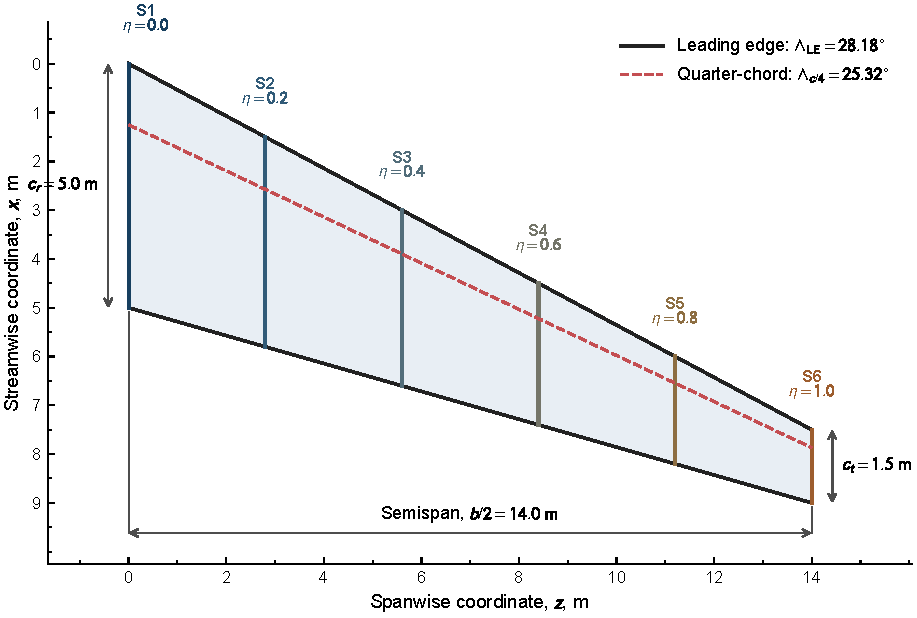
\includegraphics[width=0.84\linewidth]{II_Database_and_Preprocessing/figures/II_A_Fig01/II_A_Fig01_reference_wing_planform.pdf}
    \caption{Reference half-wing planform, principal dimensions, and spanwise locations of the six baseline airfoil sections, where $\eta=2z/b$ denotes the normalized semispan coordinate.}
    \label{fig:reference-wing-planform}
\end{figure}

\begin{figure}[!htb]
    \centering
    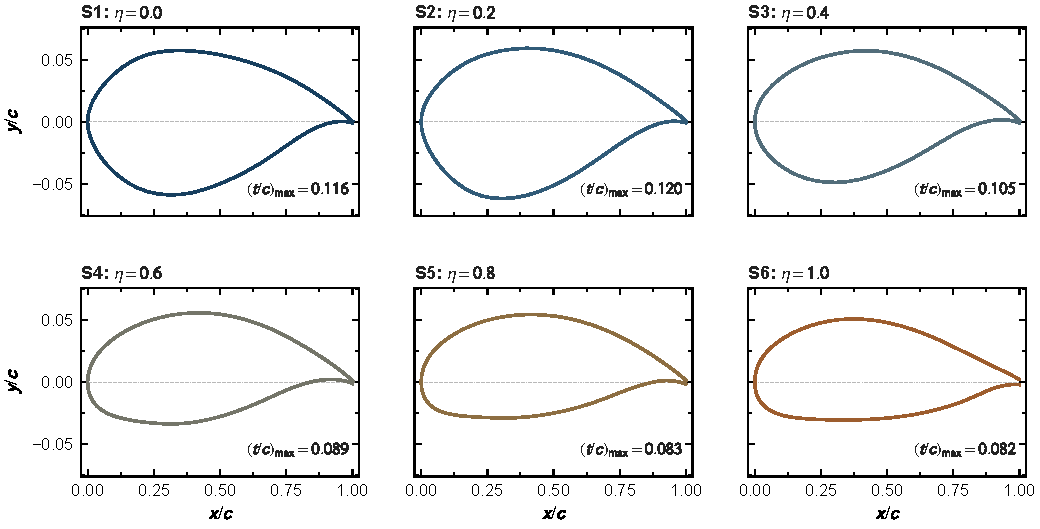
\includegraphics[width=0.98\linewidth]{II_Database_and_Preprocessing/figures/II_A_Fig02/II_A_Fig02_reference_airfoil_sections.pdf}
    \caption{Baseline airfoil profiles extracted at six spanwise stations of the reference wing and expressed in local chord-normalized coordinates.}
    \label{fig:reference-airfoil-sections}
\end{figure}

To introduce continuous shape variations while retaining the characteristics of the baseline profiles, the class--shape transformation (CST) method \cite{Kulfan2008} is employed to parameterize each airfoil section. For the upper and lower surfaces $s\in\{u,l\}$, the geometry is expressed as
\[
    \frac{y_s(\xi)}{c}
    = \xi^{1/2}(1-\xi)
      \sum_{i=0}^{4} A_{i,s}\binom{4}{i}\xi^i(1-\xi)^{4-i}
      + \xi t_s,
    \qquad \xi=\frac{x}{c},
\]
where $A_{i,s}$ denotes the corresponding Bernstein-polynomial shape coefficient and $t_s$ is the derived nondimensional trailing-edge ordinate of surface $s$. Each sampled airfoil is generated by perturbing the CST coefficients of its respective baseline section rather than by scaling a single reference airfoil. This treatment retains the differences among the spanwise sections while allowing their shapes to vary parametrically.


\subsubsection{Knowledge-Domain Databases}
\label{sec:database-architecture}
\label{sec:design-space}

The surface-pressure distribution of a finite wing reflects both the sectional aerodynamic response associated with local airfoil geometry and flow conditions and the additional three-dimensional effects of finite span, which are particularly pronounced near the wing root and tip. To characterize these contributions separately, two knowledge-domain databases are constructed using infinite-span swept wings and constant-chord finite-span wings. Their geometric and operating-condition correspondence enables the extraction of finite-span pressure corrections, as illustrated in Fig.~\ref{fig:database-architecture}.


\begin{figure}[!htb]
    \centering
    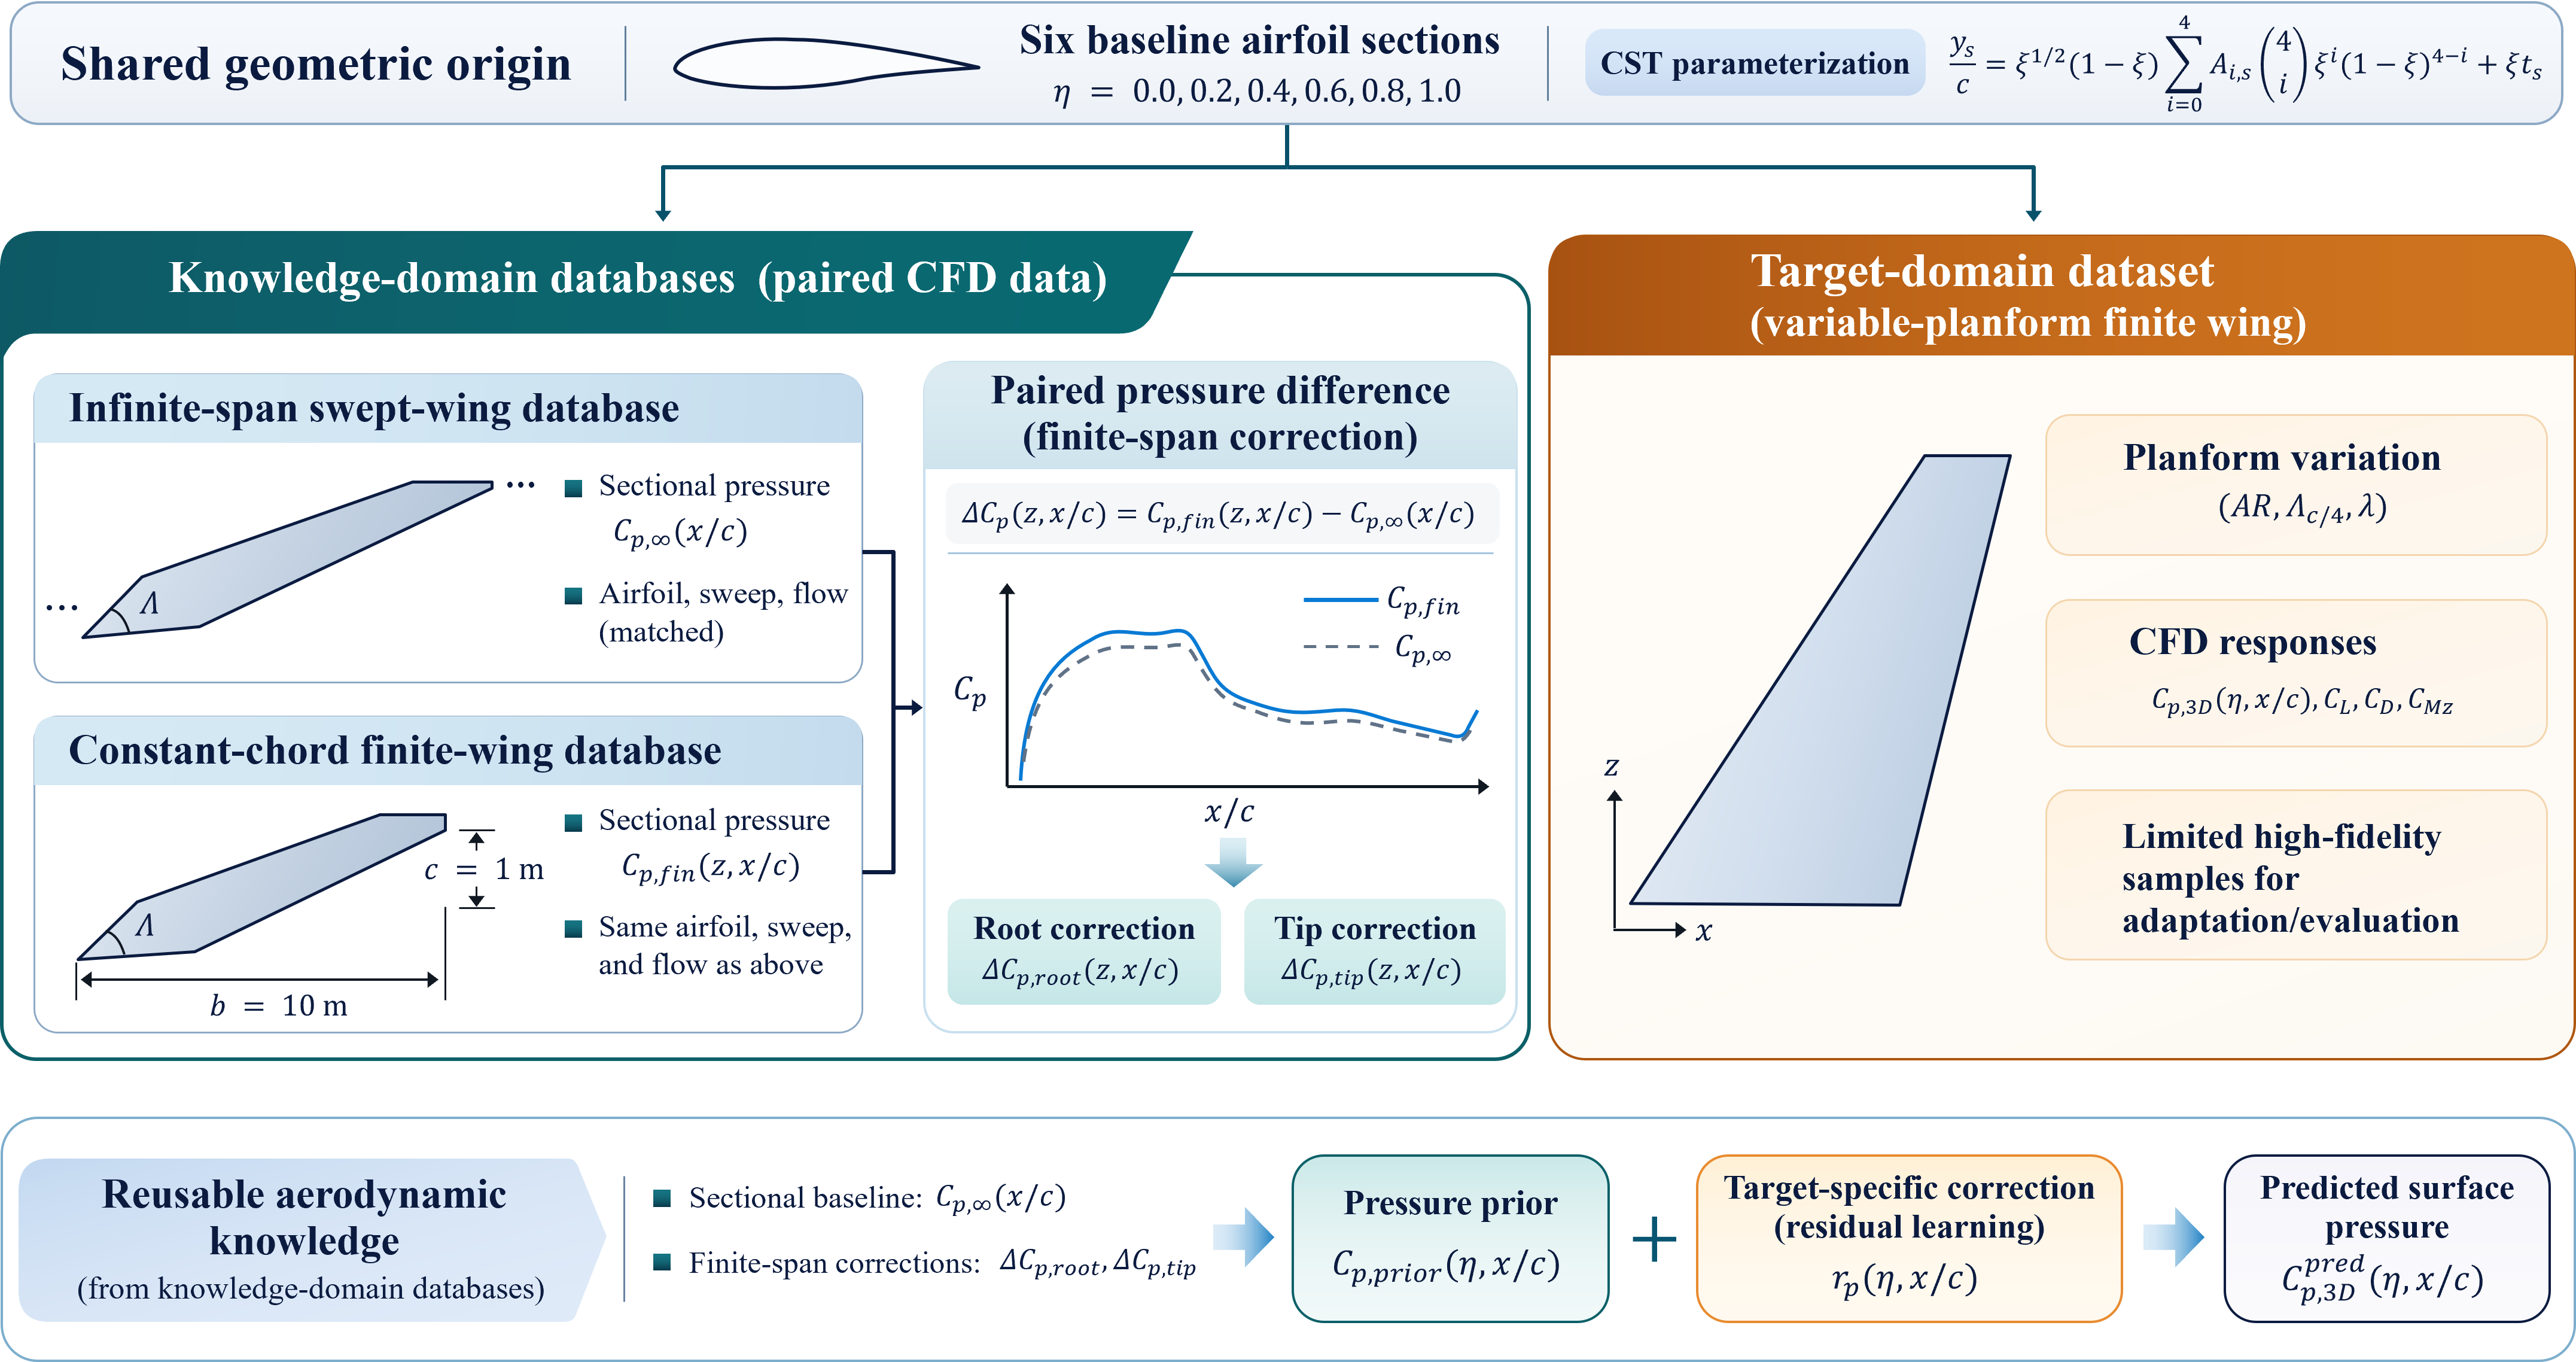
\includegraphics[width=0.98\linewidth]{II_Database_and_Preprocessing/figures/II_A_Fig03/II_A_Fig03_database_architecture.png}
    \caption{Overview of the aerodynamic databases and hierarchical knowledge transfer for finite-wing pressure prediction.}
    \label{fig:database-architecture}
\end{figure}


The infinite-span swept-wing database characterizes the baseline sectional pressure distribution $C_{p,\infty}(x/c)$ under different airfoil geometries and flow conditions. The paired constant-chord finite wings have a semispan of \SI{10}{m} and a chord of \SI{1}{m}, with the same airfoil geometry, sweep angle, and operating conditions as their infinite-span counterparts. The pressure difference associated with finite span is defined as
\begin{equation}
    \Delta C_p(z,x/c)
    = C_{p,\mathrm{fin}}(z,x/c)-C_{p,\infty}(x/c),
    \label{eq:paired-delta-cp}
\end{equation}
where $C_{p,\mathrm{fin}}(z,x/c)$ is the finite-wing sectional pressure distribution at spanwise location $z$. Because the paired calculations share the same sectional geometry and flow conditions, this difference captures the additional pressure variation associated with finite-span effects relative to the infinite-span sectional response. In view of the distinct spatial characteristics of the three-dimensional effects near the wing root and tip, the corresponding pressure differences are used separately to construct the root and tip knowledge models, denoted by $\Delta C_{p,\mathrm{root}}$ and $\Delta C_{p,\mathrm{tip}}$.

The two knowledge-domain databases share the same geometric and operating-condition sampling ranges. Five CST perturbation variables are assigned to each of the upper and lower airfoil surfaces, with normalized perturbations approximately within $[-1,1]$ and thickness-to-chord ratios primarily within $0.06$--$0.16$. The sweep angle, freestream Mach number, and angle of attack vary over $25^\circ$--$35^\circ$, $0.70$--$0.80$, and $0^\circ$--$4^\circ$, respectively, while the nominal Reynolds-number sampling range is $6.0\times10^6$--$3.0\times10^7$. The realized Reynolds numbers in the infinite-span sectional database range from approximately $5.68\times10^6$ to $3.0\times10^7$. Latin hypercube sampling (LHS) is used to sample the geometric and principal operating variables while preserving the correspondence between finite- and infinite-span cases. The two databases thus provide complementary sectional pressure and finite-span correction information for the subsequent construction of hierarchical aerodynamic priors.


\subsubsection{Target-Domain Finite-Wing Configurations and Dataset}
\label{sec:target-domain-dataset}

The two knowledge-domain databases are established independently of any specific target prediction task to extract reusable sectional aerodynamic information and regional finite-span corrections. To examine the applicability of hierarchical aerodynamic knowledge transfer with limited high-fidelity data, transonic finite wings with variable planforms are selected as a representative target domain. Compared with the constant-chord configurations used for knowledge extraction, these wings exhibit coupled variations in spanwise airfoil geometry and planform parameters, providing a setting in which to investigate the contribution of different levels of aerodynamic knowledge to three-dimensional pressure prediction.

Six spanwise airfoil sections are defined at $\eta=0.0$, $0.2$, $0.4$, $0.6$, $0.8$, and $1.0$, corresponding to the baseline stations of the reference wing. Each section is represented by five upper-surface and five lower-surface CST coefficients, yielding 60 sectional CST coefficients in total. The sectional CST coefficients are coupled through a quadratic Bernstein representation along the span, with a prescribed thickness distribution. The spanwise thickness distribution is prescribed by $t(\eta)=t_{\mathrm{tip}}+(t_{\mathrm{root}}-t_{\mathrm{tip}})(1-\eta)^p$, where $p$ controls the spanwise thickness variation.

The planform is further parameterized by aspect ratio $AR$, quarter-chord sweep angle $\Lambda_{c/4}$, and taper ratio $\lambda$, with ranges of $7.0$--$11.0$, $25^\circ$--$35^\circ$, and $0.20$--$0.40$, respectively. The root chord is fixed at \SI{5.0}{m}, and the tip chord is determined by the taper ratio. Together with freestream Mach number $M_\infty$ and angle of attack $\alpha$, varying over $0.70$--$0.80$ and $0^\circ$--$4^\circ$, respectively, the target-wing configurations are characterized by 65 parameters, comprising 60 sectional CST coefficients, three planform parameters, and two flow conditions. The principal parameters and their ranges are summarized in Table~\ref{tab:design-space}. An LHS-based sampling strategy is employed to cover the parameter space defined by the combined variations in airfoil geometry, planform, and flow conditions.

\begin{table*}[htbp]
    \centering
    \caption{Principal design variables and prescribed sampling ranges of the
    aerodynamic databases.}
    \label{tab:design-space}
    \begin{tabular}{lllll}
        \hline
        Category
        & Parameter
        & Symbol
        & Sampling range
        & Database \\
        \hline

        Operating condition
        & Mach number
        & $M_\infty$
        & $0.70$--$0.80$
        & All \\

        & Angle of attack
        & $\alpha$
        & $0^\circ$--$4^\circ$
        & All \\

        & Reynolds number
        & $Re$
        & $6.0\times10^{6}$--$3.0\times10^{7}$
        & Knowledge \\

        \hline

        Sectional geometry
        & CST perturbation
        & $\delta A_i$
        & approximately $[-1,1]$
        & All \\

        & Thickness-to-chord ratio
        & $t/c$
        & approximately $0.06$--$0.16$
        & Knowledge \\

        \hline

        Knowledge-wing geometry
        & Sweep angle
        & $\Lambda$
        & $25^\circ$--$35^\circ$
        & Knowledge \\

        & Semispan
        & $b/2$
        & \SI{10}{m}
        & Finite-wing knowledge \\

        & Chord
        & $c$
        & \SI{1}{m}
        & Finite-wing knowledge \\

        \hline

        Target-wing planform
        & Aspect ratio
        & $AR$
        & $7.0$--$11.0$
        & Target \\

        & Quarter-chord sweep angle
        & $\Lambda_{c/4}$
        & $25^\circ$--$35^\circ$
        & Target \\

        & Taper ratio
        & $\lambda$
        & $0.20$--$0.40$
        & Target \\

        & Root chord
        & $c_r$
        & \SI{5.0}{m}
        & Target \\

        \hline
    \end{tabular}
\end{table*}

The target-domain CFD data contain the three-dimensional surface-pressure distributions $C_{p,\mathrm{3D}}(\eta,x/c)$ on the upper and lower wing surfaces and the corresponding lift, drag, and pitching-moment coefficients $C_L$, $C_D$, and $C_{M_z}$. The aerodynamic coefficients are obtained directly from ADflow using the half-wing planform area and mean aerodynamic chord as the reference area and length, respectively. The pitching-moment coefficient $C_{M_z}$ is evaluated about the $z$-axis, with the moment reference point located at $(0.25c_r,0,0)$.

Independent of knowledge-domain pretraining, these high-fidelity samples are used to learn the remaining pressure discrepancy between the transferable aerodynamic prior and the target-wing response and to evaluate prediction performance with limited training data. 



% ============================================================
% B. CFD Setup and Convergence Assessment
% ============================================================
% Includes:
%   1. Numerical Method and Grid Configuration
%   2. Grid Sensitivity and Mesh Selection
%   3. Iterative Convergence Assessment
% Revised Section II.B based on the originally uploaded source.
% The grid-sensitivity table is included directly in this file so that
% replacing the B-section source also updates the medium-grid count.
% Verify the reported cell counts against the actual mesh files before submission.

\subsection{CFD Setup and Convergence Assessment}
\label{sec:cfd-setup}

\subsubsection{Numerical Method}
\label{sec:numerical-method}

The aerodynamic databases were generated using ADflow, an open-source structured multiblock finite-volume solver for compressible aerodynamic analysis \cite{Mader2020ADflow}. The steady Reynolds-averaged Navier--Stokes (RANS) equations were solved with the Spalart--Allmaras turbulence model. The wing surface was treated as an adiabatic no-slip wall, with symmetry conditions imposed on the half-wing symmetry plane and freestream conditions prescribed at the far-field boundaries. The convective terms were discretized using central differencing with scalar artificial dissipation. Each solution was initialized using Runge--Kutta iterations, followed by the approximate Newton--Krylov (ANK) algorithm described by Yildirim et al.~\cite{Yildirim2019ANK}. The solution was subsequently advanced to convergence using Newton--Krylov (NK) iterations. Twenty turbulence subiterations were performed during each nonlinear iteration. The convergence criterion was defined as a reduction of at least ten orders of magnitude in the normalized total residual, $R/R_0\leq10^{-10}$, where $R_0$ is the initial residual.

\subsubsection{Grid Configuration and Sensitivity Assessment}
\label{sec:grid-sensitivity}

The infinite-span swept-wing calculations employed a two-block structured
sectional mesh with 333 circumferential and 97 wall-normal points.
The \SI{10}{m} constant-chord finite-wing knowledge-domain cases used the
same $333\times97$ sectional resolution, with additional discretization
in the spanwise direction. The sectional mesh included 296 points along
the airfoil surface, with additional clustering near the leading and
trailing edges, and 19 points in the wake region. The near-wall spacing
was selected to maintain $y^{+}<1$. For the infinite-span configurations,
the far-field boundary was located approximately $30c$ from the airfoil,
and the wall-normal spacing increased gradually toward the far field.
Although the infinite-span and finite-wing knowledge-domain cases shared
the same sectional resolution, their full computational meshes differed
because the finite-wing calculations required spanwise discretization.

A three-level grid-refinement study was conducted before database
generation to evaluate the spatial-discretization sensitivity of the
finite-wing solutions. A representative constant-chord swept wing was
selected with a thickness-to-chord ratio of $t/c=0.1195$, a quarter-chord
sweep angle of $\Lambda_{c/4}=33.33^\circ$, a chord of $c=\SI{1}{m}$,
and a semispan of $b/2=\SI{10}{m}$. The corresponding flow condition was
$M_\infty=0.76$, $\alpha=2.0^\circ$, and $Re_c=6.1686\times10^6$.
The three-dimensional grids employed a five-block topology, a first-cell
height of $5\times10^{-6}c$, and a far-field boundary located at $50c$.
The surface mesh and the near-body symmetry-plane mesh of the medium grid
are shown in Fig.~\ref{fig:medium-grid}.

\begin{figure}[!htb]
    \centering
    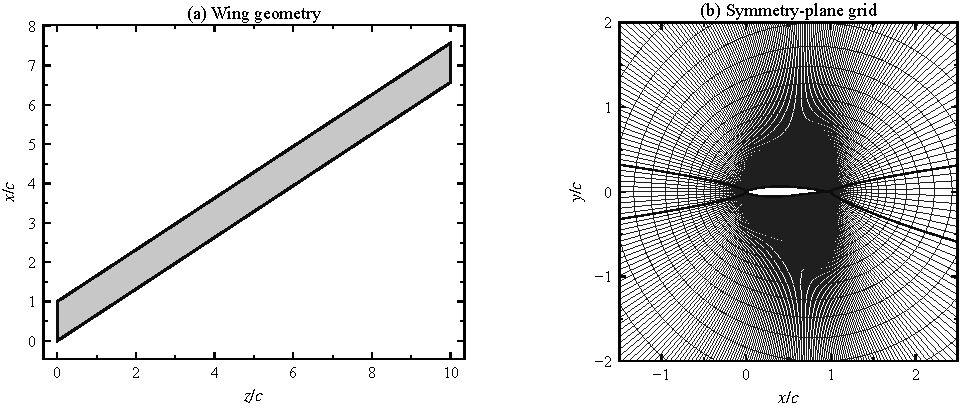
\includegraphics[width=0.94\linewidth]
        {II_Database_and_Preprocessing/figures/II_B_Fig04/II_B_Fig04_medium_grid.pdf}
    \caption{Medium grid used for the finite-wing calculations:
    (a) planform surface mesh and (b) near-body symmetry-plane volume mesh.}
    \label{fig:medium-grid}
\end{figure}

The coarse, medium, and fine grids retained the same block topology,
surface-node distribution strategy, near-wall spacing, and far-field
extent, while their resolutions were varied as summarized in
Table~\ref{tab:grid-sensitivity}. Here, $N_c$, $N_s$, and $N_n$ denote
the sectional (circumferential), spanwise, and wall-normal point counts,
respectively. The medium grid employed a $333\times97\times97$
resolution, including the same $333\times97$ sectional point counts as
the knowledge-domain meshes.

% The source manuscript reported 3.113 million cells for its medium grid.
% This number is retained pending confirmation from the corrected mesh log.
\begin{table}[!htb]
    \centering
    \caption{Grid sensitivity of the representative swept-wing case.}
    \label{tab:grid-sensitivity}
    \begingroup
    \setlength{\tabcolsep}{3pt}
    \footnotesize
    \resizebox{\linewidth}{!}{%
        \begin{tabular}{lcccccccc}
            \hline
            Grid & $N_c\times N_s\times N_n$ & Cells ($10^6$)
            & $C_L$ & $C_D$ & $C_{M_z}$
            & $|\Delta C_L|$ (\%) & $|\Delta C_D|$ (\%)
            & $|\Delta C_{M_z}|$ (\%) \\
            \hline
            Coarse & $261\times81\times81$ & 1.828
            & 0.390022 & 0.0116301 & 1.351364 & 0.263 & 0.213 & 0.269 \\
            Medium & $333\times97\times97$ & 3.113
            & 0.390872 & 0.0116498 & 1.354607 & 0.045 & 0.044 & 0.030 \\
            Fine & $375\times117\times117$ & 5.378
            & 0.391049 & 0.0116549 & 1.355009 & --- & --- & --- \\
            \hline
        \end{tabular}%
    }
    \endgroup
\end{table}

The integrated aerodynamic coefficients exhibited monotonic convergence
with grid refinement. Relative to the fine-grid solution, the medium-grid
differences were 0.045\% in $C_L$, 0.044\% in $C_D$, and 0.030\% in
$C_{M_z}$. The reported cell count increased by a factor of 1.73 from
the medium to the fine grid, while the changes in all three integrated
coefficients remained below 0.05\%. The medium grid was therefore
selected for database generation, reducing the reported cell count by
42.1\% relative to the fine grid while retaining nearly identical
integrated aerodynamic coefficients.

Because the surface pressure coefficient is a primary prediction target
of the present study, grid sensitivity was also assessed using local
pressure distributions. Figure~\ref{fig:cp-grid-sensitivity} compares
the $C_p$ distributions obtained on the three grids at representative
spanwise locations of $z=0.5$, $5.0$, and $9.5$~m.

\begin{figure}[!htb]
    \centering
    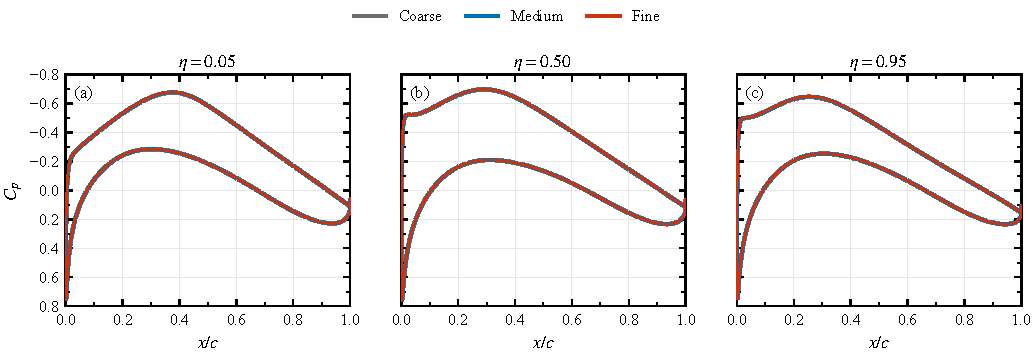
\includegraphics[width=0.94\linewidth]
        {II_Database_and_Preprocessing/figures/II_B_Fig05/II_B_Fig05_cp_grid_sensitivity.pdf}
    \caption{Pressure-coefficient distributions obtained on the coarse,
    medium, and fine grids at spanwise stations of $z=0.5$, $5.0$, and
    $9.5$~m for the representative finite-wing configuration.}
    \label{fig:cp-grid-sensitivity}
\end{figure}

The three locations exhibit distinct sectional loading characteristics,
whereas the medium- and fine-grid pressure distributions remain closely
matched. Together with the convergence of the integrated aerodynamic
coefficients, this agreement supports the use of the medium grid for the
finite-wing database calculations.

\subsubsection{Iterative Convergence Assessment}
\label{sec:solver-convergence}

In addition to the grid-sensitivity analysis, iterative convergence was
examined for the medium-grid verification case. Figure~\ref{fig:iterative-convergence}
shows the evolution of the normalized total residual, $R/R_0$, during
solution convergence.

\begin{figure}[!htb]
    \centering
    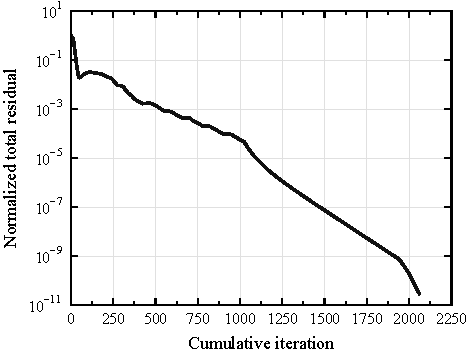
\includegraphics[width=0.72\linewidth]
        {II_Database_and_Preprocessing/figures/II_B_Fig06/II_B_Fig06_iterative_convergence.pdf}
    \caption{Convergence history of the normalized total residual for the
    medium-grid verification case.}
    \label{fig:iterative-convergence}
\end{figure}

The medium-grid solution converged after 2060 cumulative nonlinear
iterations. The normalized total residual decreased by 10.52 orders of
magnitude, satisfying the prescribed criterion of $R/R_0\leq10^{-10}$.
Over the final five reported iterations, the peak-to-peak variations in
$C_L$, $C_D$, and $C_{M_z}$ were 0.000059\%, 0.000013\%, and
0.000067\%, respectively. These variations were substantially smaller
than the corresponding medium-to-fine grid differences, indicating that
the remaining iterative error was negligible relative to the assessed
spatial-discretization sensitivity.



% ============================================================
% C. Surface Data Preprocessing
% ============================================================

\subsection{Surface Data Preprocessing}
\label{sec:data-preprocessing}

To obtain consistent sectional representations across the aerodynamic databases, the upper and lower airfoil surfaces were processed separately using local chord-normalized coordinates. The original CFD nodes were ordered by $\xi=x/c$, and nearly coincident chordwise locations were merged before interpolation. Both surface geometry and pressure coefficients were resampled using shape-preserving piecewise cubic Hermite interpolation (PCHIP) \cite{FritschButland1984}, which limits spurious overshoots when interpolating pressure distributions with steep local gradients.

A total of 100 chordwise nodes were allocated between the upper and lower surfaces. Under transonic conditions, the upper surface generally exhibits more pronounced suction peaks and sharper pressure gradients, including possible shock-induced pressure variations, whereas the lower-surface pressure distribution is typically smoother. To provide higher resolution in regions of stronger pressure variation, more nodes were assigned to the upper surface using prescribed importance weights of $\omega_u=1.8$ and $\omega_l=1.0$, resulting in 64 upper-surface and 36 lower-surface nodes.

For each surface, the chordwise nodes were concentrated near the leading edge, with the spacing increasing smoothly toward a uniform-spacing region downstream. The interval widths were prescribed using a fifth-order smoothstep function:
\begin{equation}
    w_{s,j}=1+(r_s-1)S\left(\min\left(\frac{j}{K_s},1\right)\right),\qquad S(t)=6t^5-15t^4+10t^3,
    \label{eq:chordwise-spacing}
\end{equation}
where $s\in\{u,l\}$, $j=0,\ldots,N_s-2$, $K_s=\max\{1,\lfloor\rho_s(N_s-2)\rfloor\}$, and $r_s$ controls the ratio of downstream to initial spacing. The chordwise node coordinates were obtained by normalizing the cumulative interval widths and mapping them to the prescribed sampling interval. The distribution parameters were $(\rho_u,r_u)=(0.28,5.0)$ and $(\rho_l,r_l)=(0.24,4.0)$ for the upper and lower surfaces, respectively. The resulting chordwise discretization is shown in Fig.~\ref{fig:chordwise-nodes}, which compares the node locations and adjacent-node spacing on the upper and lower surfaces.

\begin{figure}[!htb]
    \centering
    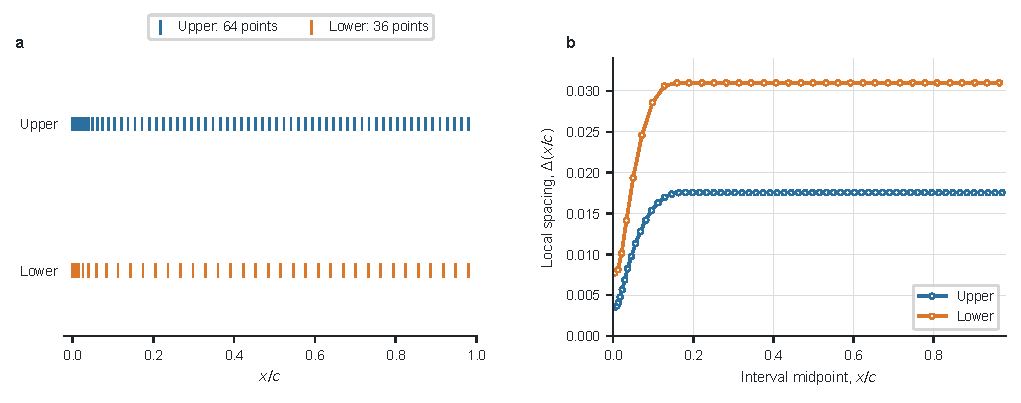
\includegraphics[width=0.94\linewidth]{II_Database_and_Preprocessing/figures/II_C_Fig07/II_C_Fig07_chordwise_nodes.pdf}
    \caption{Chordwise discretization of the upper and lower airfoil surfaces: (a) node locations and (b) adjacent-node spacing.}
    \label{fig:chordwise-nodes}
\end{figure}

For finite-wing configurations, the original CFD sectional locations were retained without additional spanwise interpolation. Following chordwise resampling, the paired infinite-span and constant-chord finite-wing pressure distributions share identical chordwise coordinates, allowing the finite-span pressure corrections in Eq.~\eqref{eq:paired-delta-cp} to be calculated by pointwise subtraction. The upper- and lower-surface pressure data were retained separately for subsequent aerodynamic modeling.



% ============================================================
% III. Hierarchical Aerodynamic Knowledge Transfer
% ============================================================

\section{Hierarchical Aerodynamic Knowledge Transfer}
\label{sec:methodology}


% A. Problem Formulation and Overall Framework

\subsection{Problem Formulation and Overall Framework}
\label{sec:method-overview}

Predicting the surface pressure of transonic wings with limited high-fidelity data requires exploiting transferable sectional aerodynamic information while accounting for three-dimensional flow effects. To address this challenge, a hierarchical knowledge-transfer method is developed to separately represent the baseline sectional pressure response and localized pressure corrections near the wing root and tip. These knowledge components are transferred to the target wing to construct a three-dimensional pressure prior, while a residual model trained on limited target-domain CFD data learns the remaining pressure discrepancy.

For a wing with spanwise-varying airfoil geometry and planform parameters, let $\eta=z/(b/2)$ denote the normalized spanwise coordinate and $\xi=x/c(\eta)$ the local chord-normalized coordinate. The predicted surface pressure coefficient is expressed as
\begin{equation}
    \widehat{C}_{p,s}^{3D}(\eta,\xi)
    = C_{p,s}^{\mathrm{prior}}(\eta,\xi)
    + \widehat{R}_{p,s}^{\mathrm{tar}}(\eta,\xi),
    \qquad s\in\{u,l\},
    \label{eq:hierarchical-pressure-decomposition}
\end{equation}
where $u$ and $l$ denote the upper and lower surfaces, respectively. The pressure prior $C_{p,s}^{\mathrm{prior}}$ combines the baseline sectional response with regional finite-span corrections, whereas $\widehat{R}_{p,s}^{\mathrm{tar}}$ represents the residual pressure discrepancy learned from target-domain data.

The overall framework is illustrated in Fig.~\ref{fig:hierarchical-framework}. A sectional baseline model is pretrained using infinite-span swept-wing data, while separate root and tip correction models are developed from paired finite- and infinite-span pressure differences. For a given target-wing geometry and flow condition, the pretrained knowledge models are combined through sectionwise mapping, spanwise gating, and amplitude calibration to construct the pressure prior. With the knowledge models frozen, a target-domain residual network incorporates geometric and flow information, the pressure prior, and pretrained sectional features to predict the remaining pressure correction. High-fidelity target-domain CFD data provide supervision during training, whereas inference requires only the target geometry and flow conditions. The resulting surface-pressure predictions are further used as inputs to separately trained aerodynamic-coefficient regression models.

\begin{figure*}[t]
    \centering
    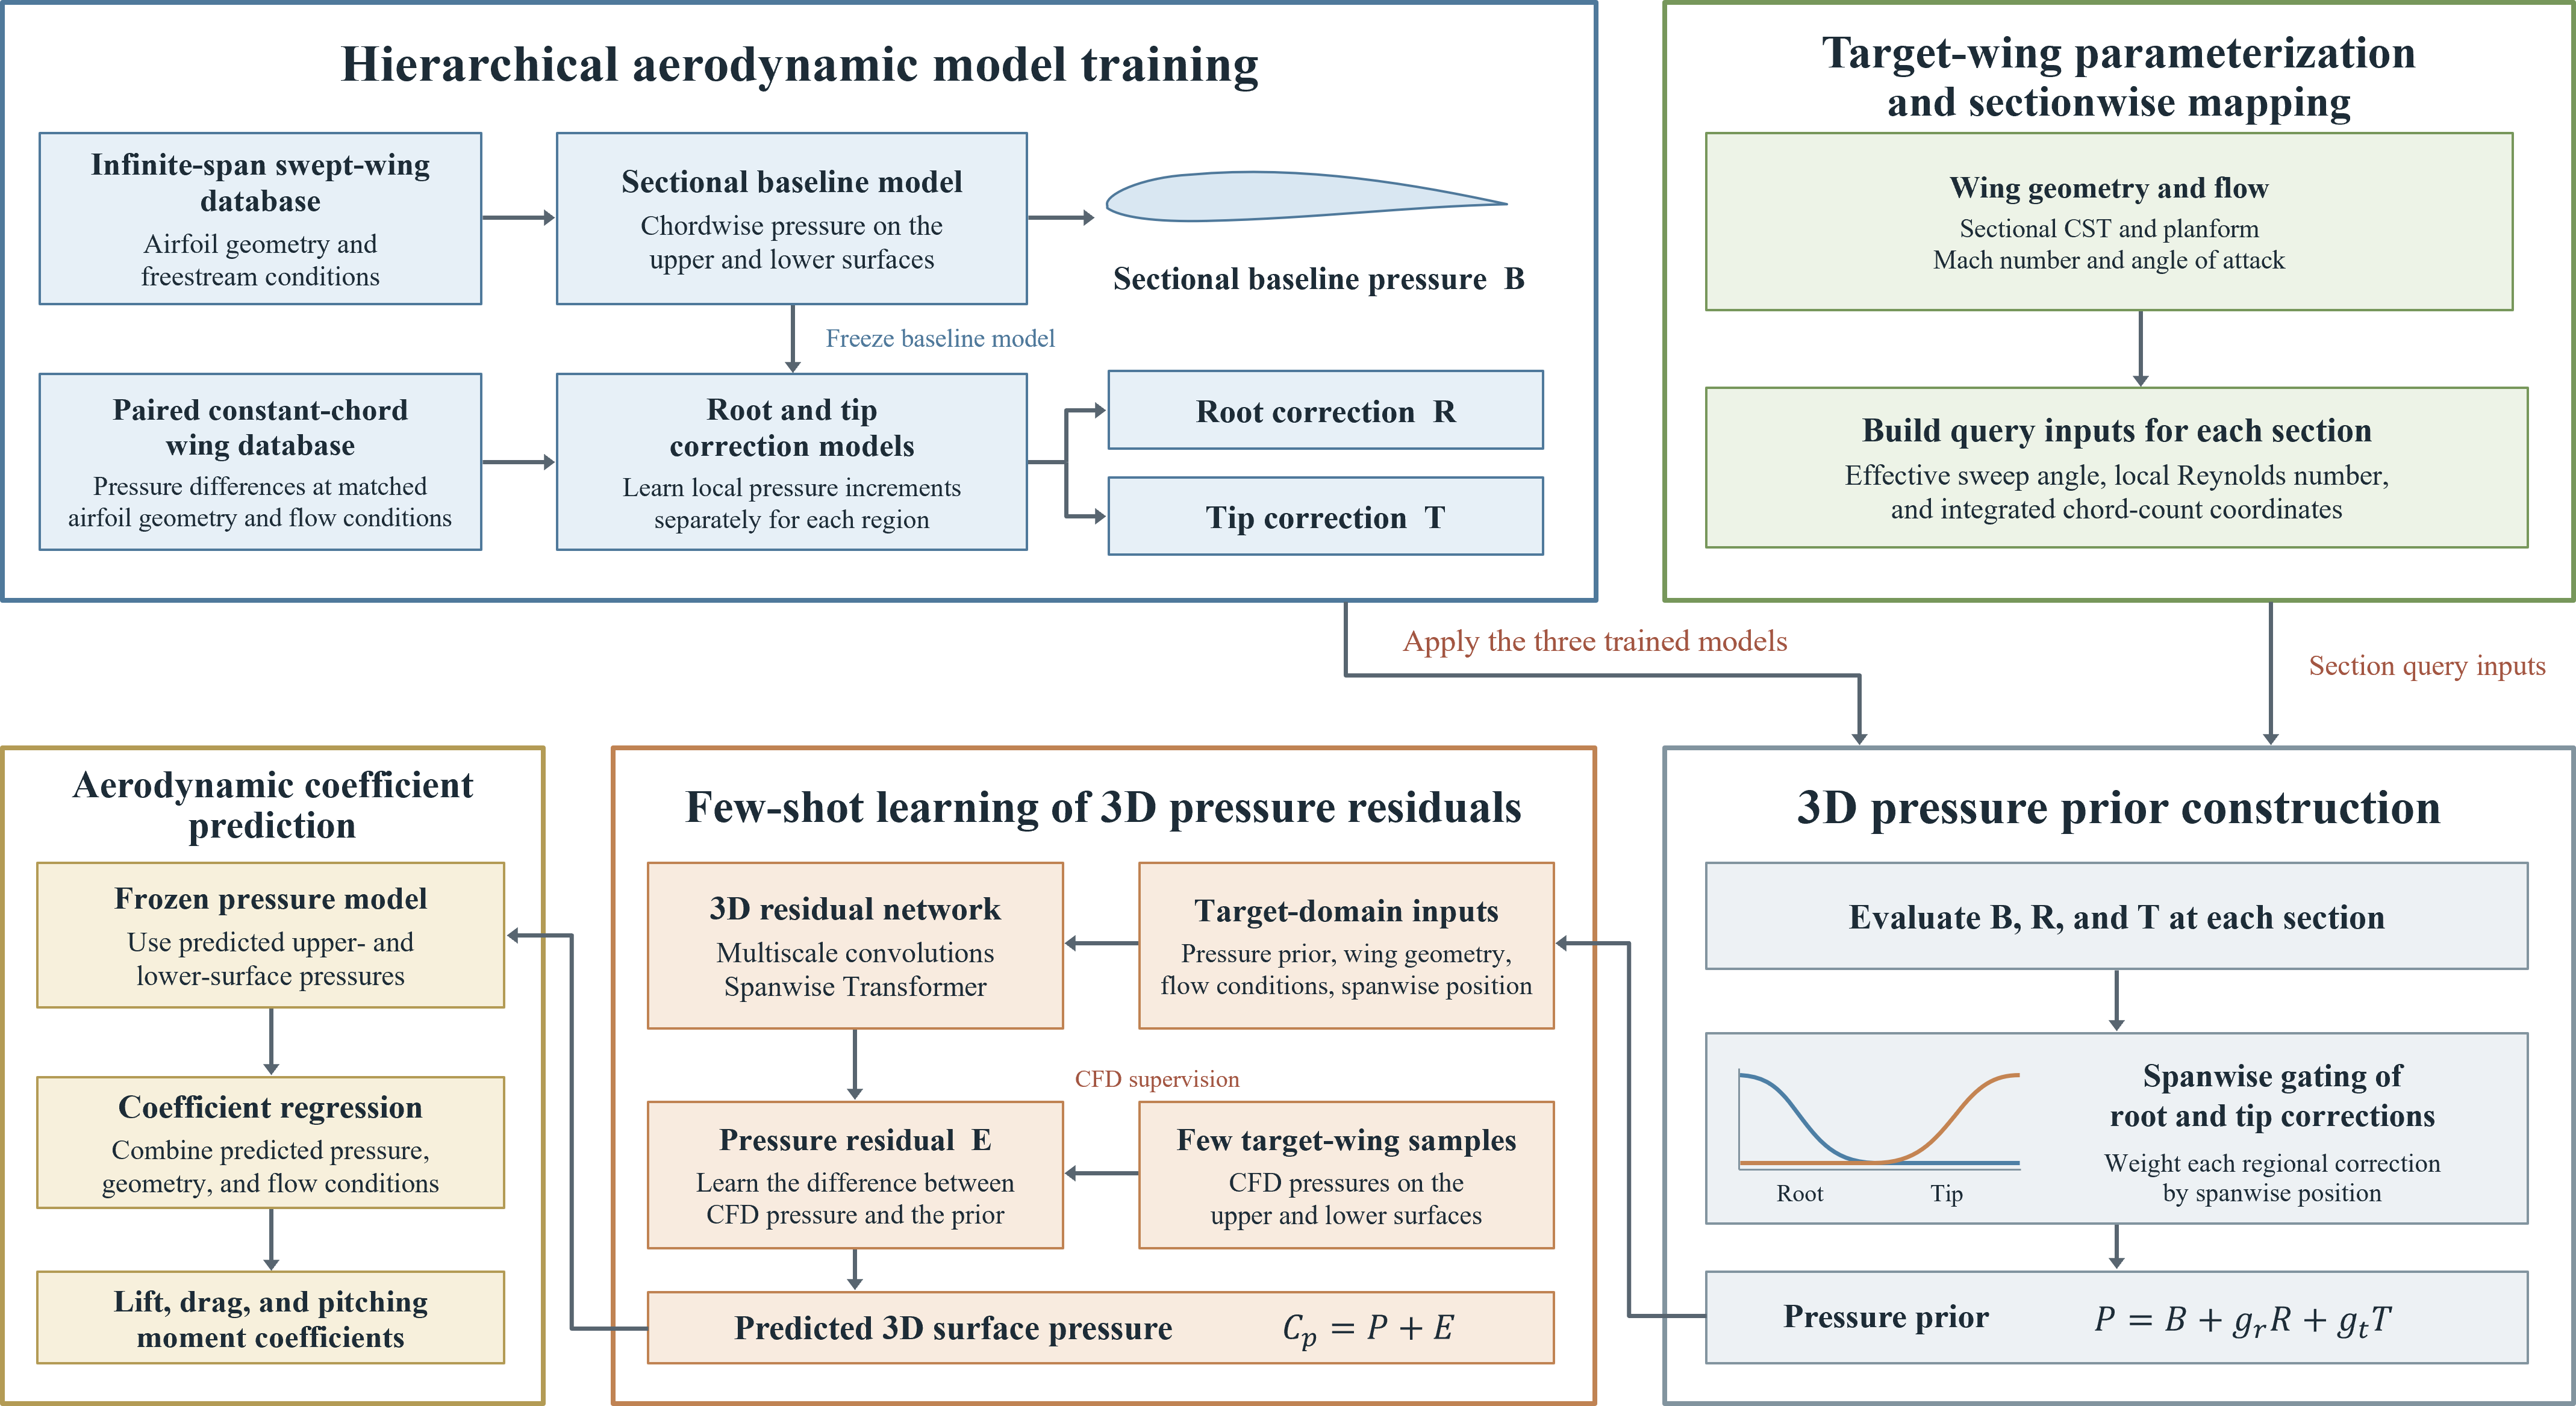
\includegraphics[width=\textwidth]{III_Knowledge_Transfer/figures/III_A_Fig08/III_A_Fig08_hierarchical_framework_v2.png}
    \caption{Hierarchical aerodynamic knowledge-transfer framework for wing surface-pressure prediction and aerodynamic-coefficient regression.}
    \label{fig:hierarchical-framework}
\end{figure*}



% B. Hierarchical Aerodynamic Knowledge Learning

\subsection{Hierarchical Aerodynamic Knowledge Learning}
\label{sec:knowledge-learning}

The source-domain aerodynamic knowledge is represented at two complementary levels: the baseline sectional pressure response and the regional pressure corrections associated with finite-span effects. The sectional model provides baseline pressure distributions and reusable aerodynamic features, while the regional models learn root and tip pressure corrections conditioned on the sectional response. Their transfer and spatial combination on the target wing are described in Sec.~\ref{sec:knowledge-projection}.

\subsubsection{Sectional Baseline Pressure Model}
\label{sec:sectional-baseline}

The sectional baseline model predicts the pressure distributions of infinite-span swept wings from airfoil geometry and flow conditions. The upper and lower surfaces are represented on separate chordwise grids, each containing three input channels: the normalized surface ordinate $y/c$, an affinely rescaled chordwise coordinate $x/c$, and the logarithm of the local nodal spacing relative to its mean. The flow-condition vector is defined as $\boldsymbol{\mu}=[M_\infty,\alpha,\Lambda,\log_{10}(Re/10^{7})]^{\mathsf T}$. The geometric ordinates and flow conditions are standardized using statistics from the training partition. The model predicts the upper- and lower-surface pressure distributions as
\begin{equation}
    \left(\widehat{\mathbf C}_{p,u}^{\mathrm{sec}},
          \widehat{\mathbf C}_{p,l}^{\mathrm{sec}}\right)
    =\mathcal F_{\mathrm{sec}}\!\left(\mathbf G_u,\mathbf G_l,\boldsymbol{\mu}\right),
    \label{eq:sectional-baseline-map}
\end{equation}
where $\mathbf G_s\in\mathbb R^{3\times N_s}$ denotes the coordinate representation of surface $s\in\{u,l\}$, and $N_s$ is the corresponding number of chordwise nodes.

The network architecture is illustrated in Fig.~\ref{fig:sectional-architecture}. It consists of two surface-specific convolutional branches, a shared flow-condition encoder, and a global feature-fusion module. The condition encoder maps the four-dimensional flow-condition vector into a 128-dimensional embedding $\mathbf h$. For each surface, an initial one-dimensional convolution maps the three input channels to 128 feature channels, followed by eight FiLM-modulated residual blocks with dilation factors $(1,2,4,1,2,4,1,2)$. The flow-condition embedding modulates the intermediate features through feature-wise linear modulation (FiLM), expressed as
\begin{equation}
    \widetilde{\mathbf H}
    =\left[\mathbf 1+\boldsymbol\gamma(\mathbf h)\right]
    \odot \operatorname{GN}(\mathbf H)+\boldsymbol\beta(\mathbf h),
    \label{eq:sectional-film}
\end{equation}
where $\operatorname{GN}$ denotes group normalization, and $\boldsymbol\gamma$ and $\boldsymbol\beta$ are condition-dependent channelwise modulation parameters. The residual blocks extract chordwise features at multiple receptive-field scales without downsampling, preserving the original nodal resolution of each surface.

To incorporate information from both surfaces, the extracted features are independently aggregated into 128-dimensional vectors through quadrature-weighted pooling. These vectors are concatenated with the condition embedding $\mathbf h$ and passed through a shared fusion network with dimensions $384\rightarrow256\rightarrow256$. The resulting global representation is divided into two 128-dimensional feature increments, which are broadcast along the corresponding chordwise grids and added to the surface-specific features. Separate prediction heads then map the fused features to the upper- and lower-surface pressure coefficients. This design preserves independent surface representations while allowing the two branches to exchange global aerodynamic information.

The sectional model is trained using the CFD pressure distributions of the infinite-span swept-wing database. The training objective is the equally weighted mean squared error of the upper- and lower-surface predictions, excluding the first chordwise node on each surface because of discontinuities in the corresponding CFD labels. After pretraining, the model provides baseline sectional pressure predictions for the regional correction models, while its intermediate features are retained for subsequent target-domain residual learning in Sec.~\ref{sec:target-residual}.

\begin{figure*}[t]
    \centering
    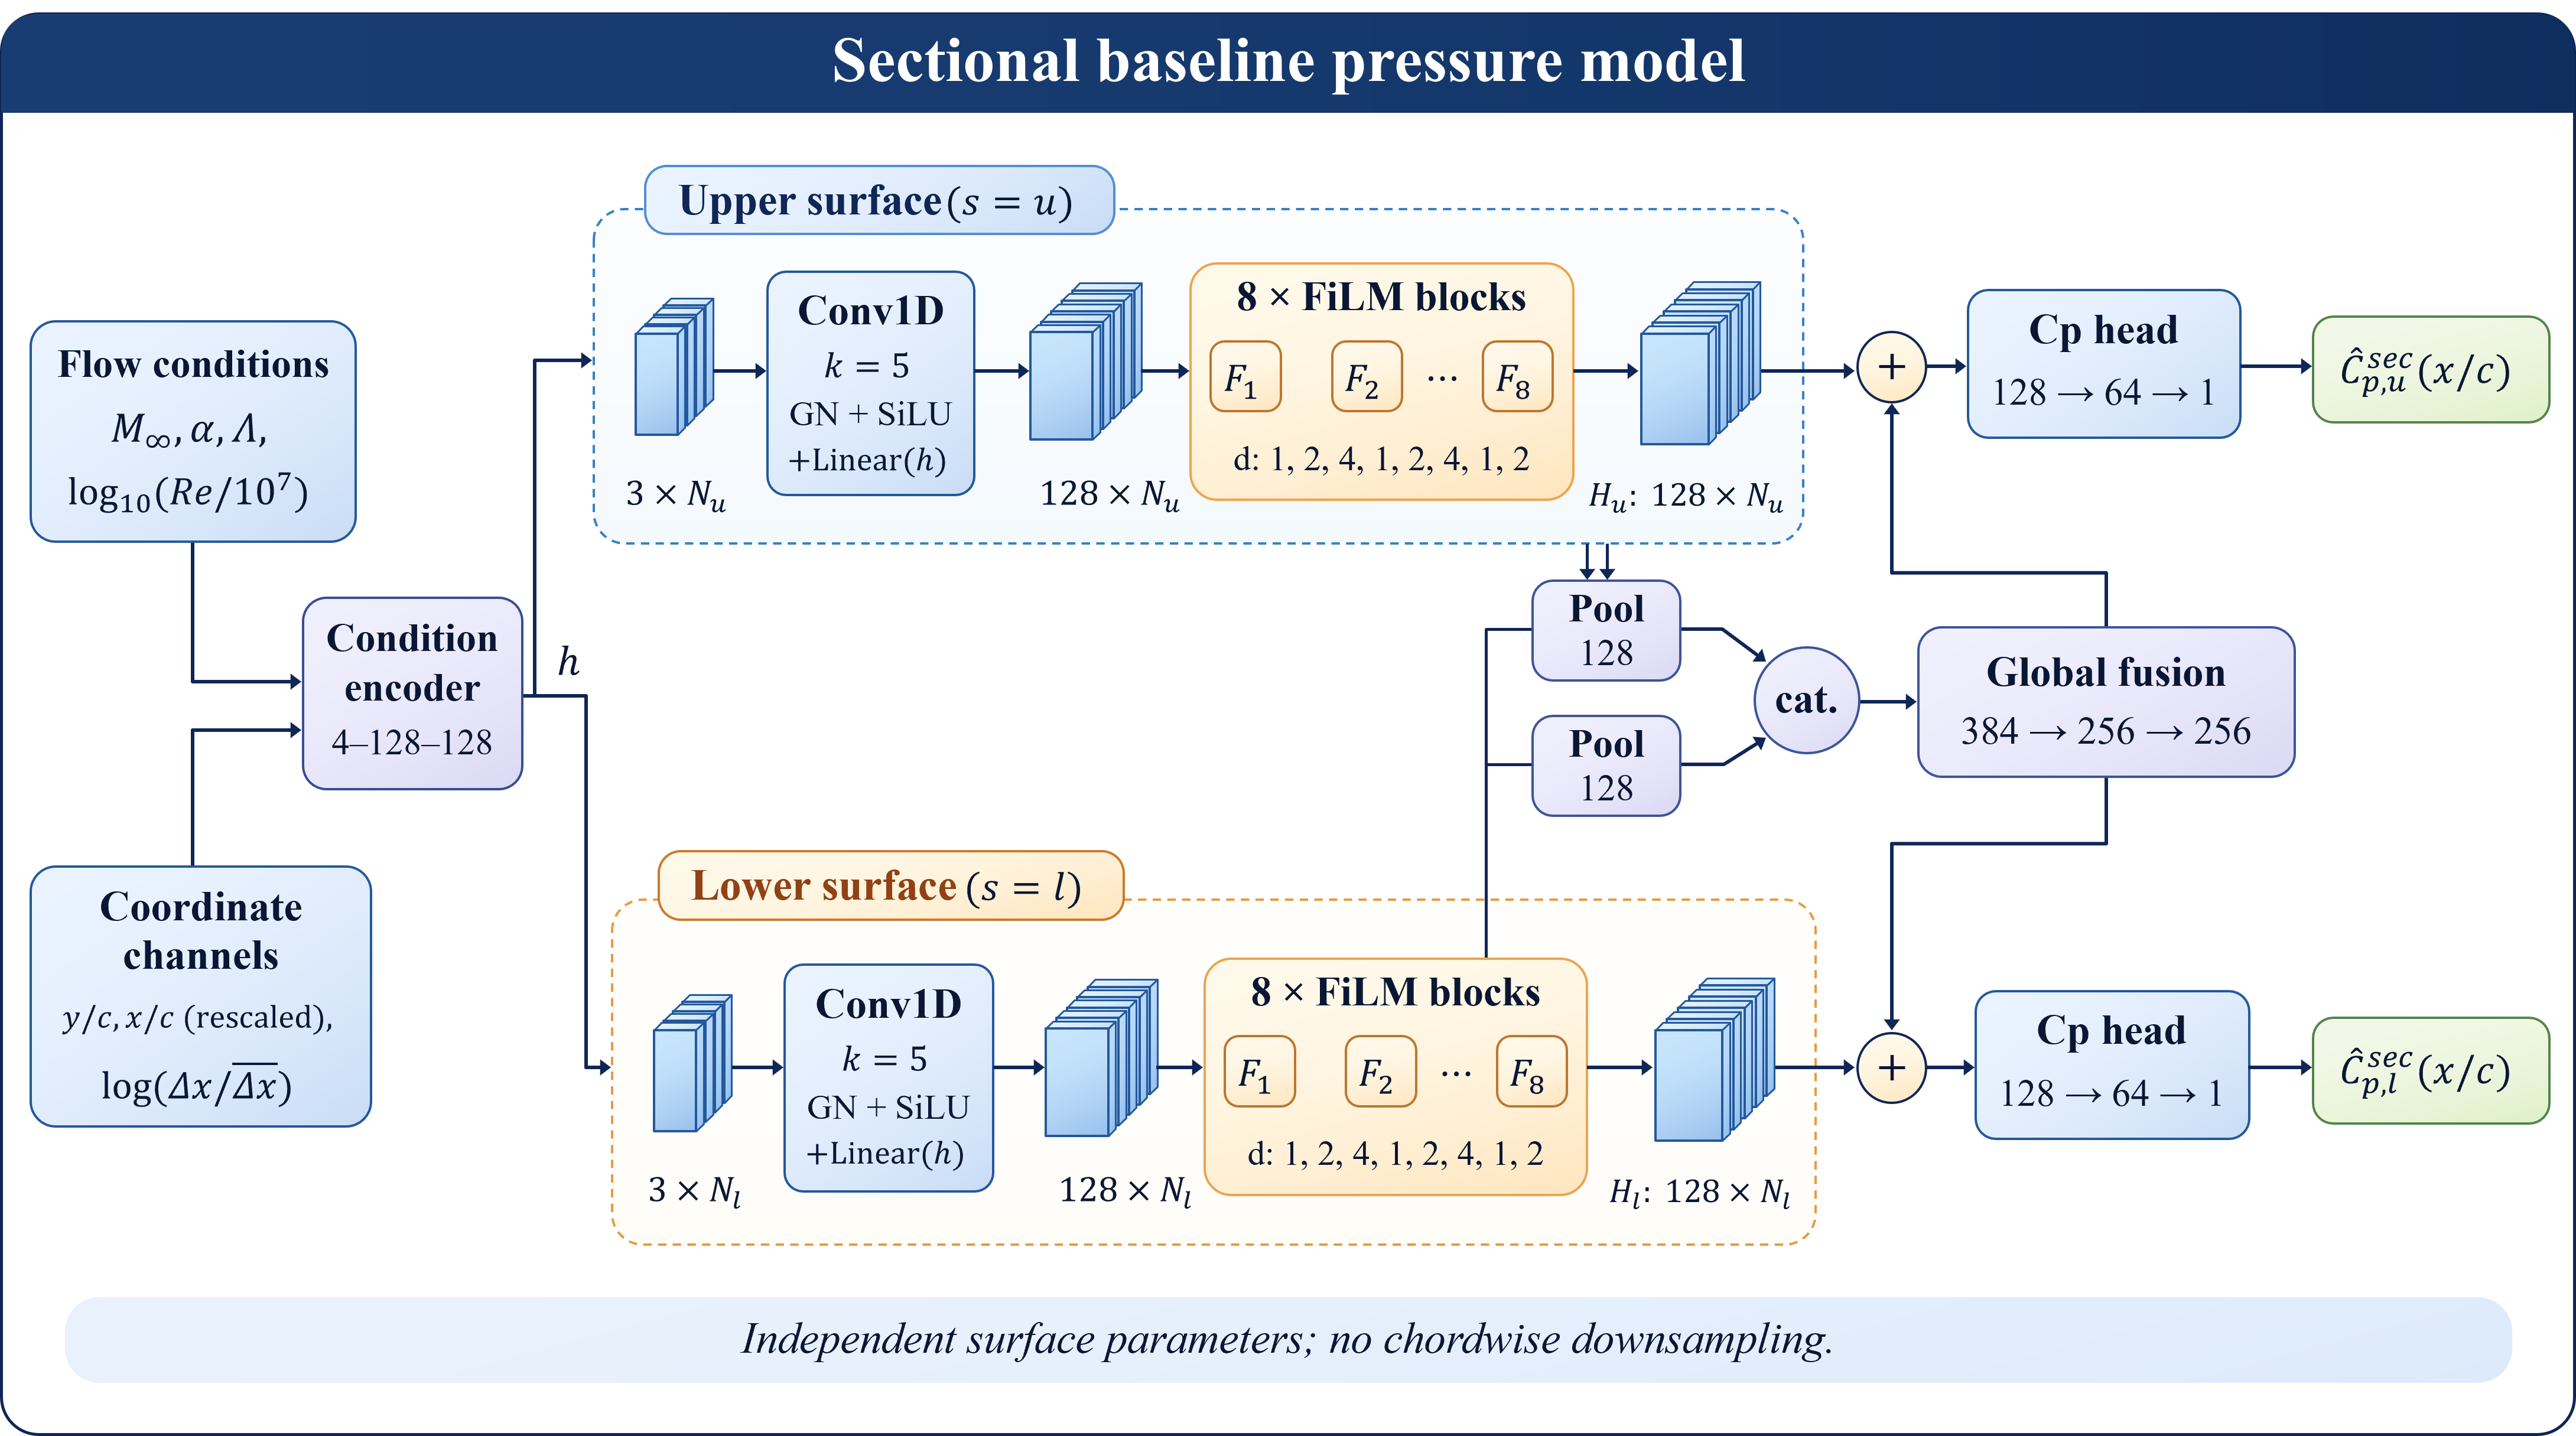
\includegraphics[width=0.98\textwidth]{III_Knowledge_Transfer/figures/III_B_Fig09/III_B_Fig09_sectional_architecture.png}
    \caption{Architecture of the sectional baseline pressure model with surface-specific convolutional branches and shared global feature fusion.}
    \label{fig:sectional-architecture}
\end{figure*}



\subsubsection{Regional Finite-Span Correction Models}
\label{sec:regional-correction}

The regional correction models are developed to capture pressure variations associated with finite-span effects near the wing root and tip that are not represented by the sectional baseline response. For geometrically and aerodynamically matched finite- and infinite-span CFD cases, the pressure discrepancy is defined as
\begin{equation}
    \Delta C_{p,s}^{\mathrm{CFD}}(d,\xi)
    = C_{p,s}^{\mathrm{fin,CFD}}(d,\xi)
    - C_{p,s}^{\infty,\mathrm{CFD}}(\xi),
    \qquad s\in\{u,l\},
    \label{eq:regional-cfd-discrepancy}
\end{equation}
where $\xi=x/c$ is the normalized chordwise coordinate and $d$ denotes the distance from the corresponding spanwise boundary. The correction targets are obtained directly from paired CFD solutions rather than from discrepancies relative to the learned sectional predictions.

For the root region, the correction model incorporates airfoil geometry, flow conditions, the normalized root-distance coordinate $d_r$, and the upper- and lower-surface pressure distributions predicted by the pretrained sectional model. The corresponding mapping is expressed as
\begin{equation}
    \left(\widehat{\Delta\mathbf C}_{p,r,u},
          \widehat{\Delta\mathbf C}_{p,r,l}\right)
    =\mathcal F_r\!\left(
    \mathbf G_u,\mathbf G_l,\boldsymbol\mu,d_r,
    \widehat{\mathbf C}_{p,u}^{\mathrm{sec}},
    \widehat{\mathbf C}_{p,l}^{\mathrm{sec}}
    \right),
    \label{eq:root-correction-map}
\end{equation}
where the sectional model remains frozen during regional training. Its predicted pressure distributions provide aerodynamic conditioning information, while the root-distance coordinate characterizes the spanwise variation in the pressure correction.

The root-region correction network is illustrated in Fig.~\ref{fig:regional-architecture}. To accommodate the different chordwise discretizations of the upper and lower surfaces, the lower-surface geometry and predicted sectional pressure are interpolated onto the upper-surface grid. The resulting input contains four surface channels, comprising the upper- and lower-surface ordinates and their corresponding sectional pressure predictions, together with five broadcast conditioning channels and one normalized chordwise-coordinate channel. These ten channels are processed by a Conv1D stem followed by six multiscale residual blocks with dilation factors $(1,2,4,2,1,2)$. A zero-initialized two-channel prediction head produces pressure corrections for both surfaces on the common grid, after which the lower-surface correction is interpolated back to its original chordwise grid. Each spanwise section is processed independently.

The multiscale residual blocks combine conventional and dilated convolutions with channel mixing and residual connections to extract pressure-discrepancy features at different chordwise scales. The correction model is trained using an unweighted pointwise mean squared error over the retained upper- and lower-surface nodes, without additional shock- or gradient-dependent weighting. An analogous model is trained for the tip region to obtain $\widehat{\Delta\mathbf C}_{p,t}$. 

\begin{figure*}[t]
    \centering
    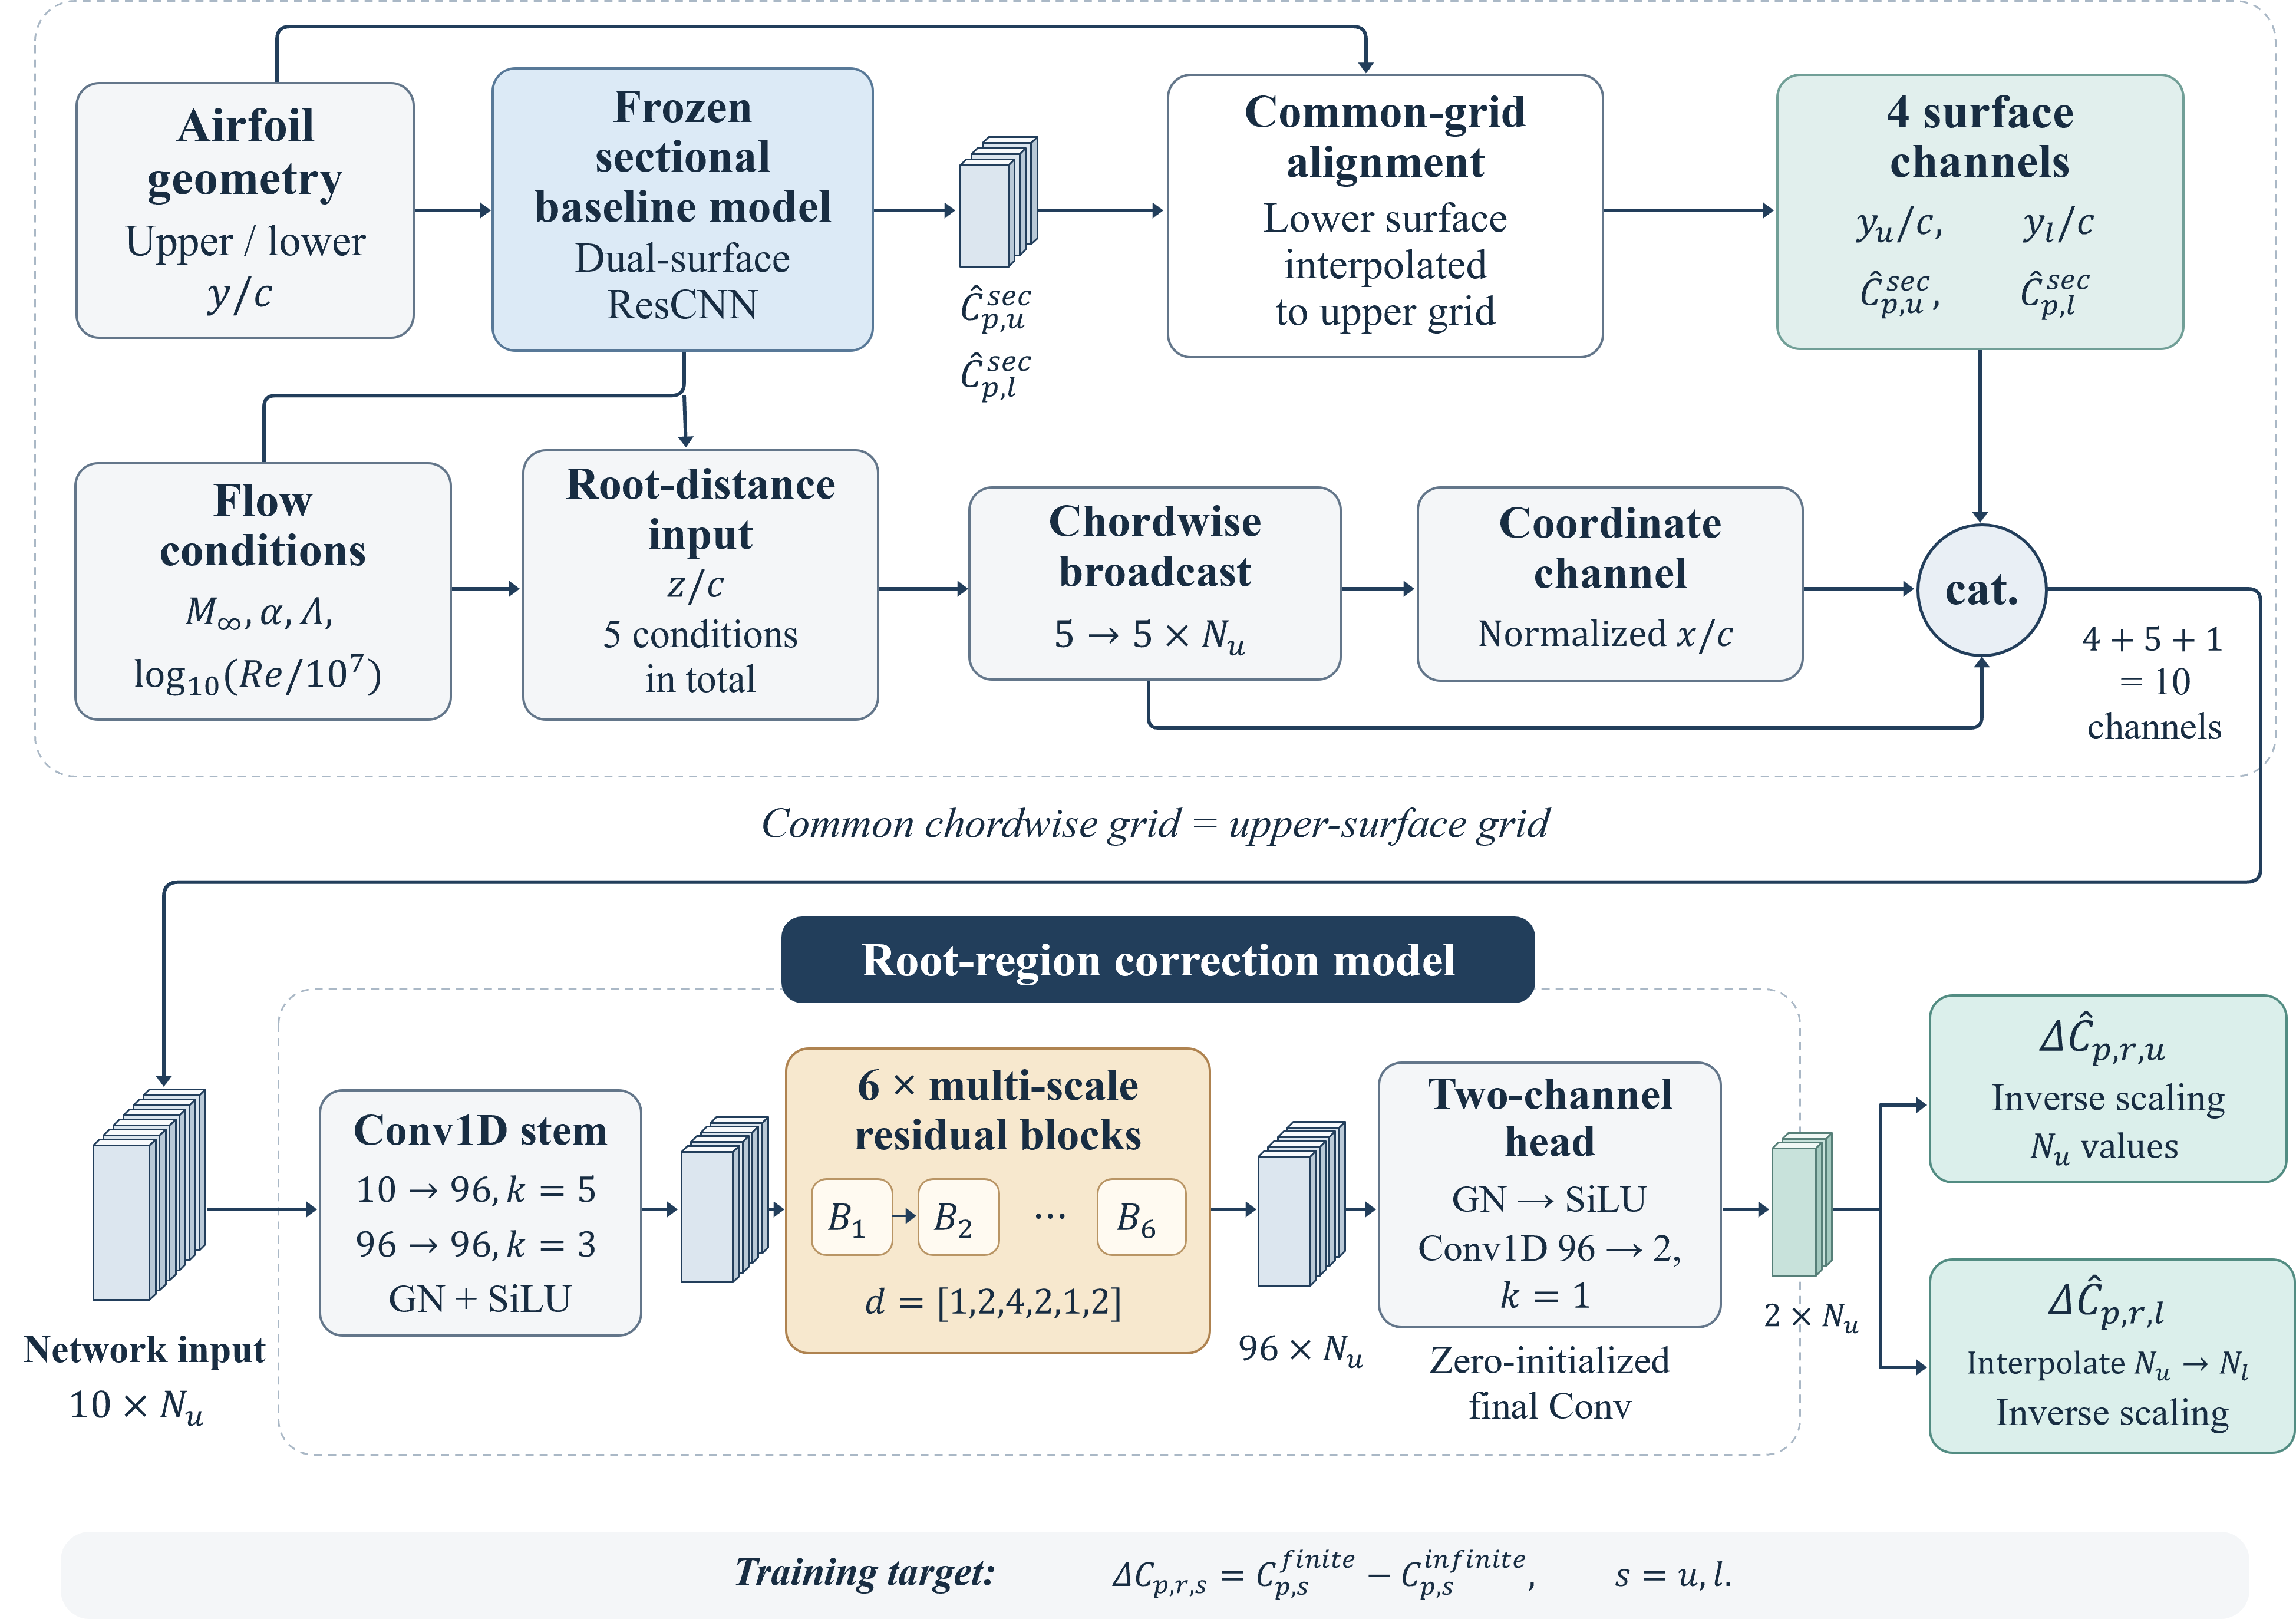
\includegraphics[width=\textwidth]{III_Knowledge_Transfer/figures/III_B_Fig10/III_B_Fig10_regional_architecture.png}
    \caption{Architecture of the root-region pressure-correction model conditioned on pretrained sectional predictions.}
    \label{fig:regional-architecture}
\end{figure*}



% C. Cross-Dimensional Knowledge Transfer

\subsection{Cross-Dimensional Knowledge Projection and Pressure-Prior Construction}
\label{sec:knowledge-projection}

The pretrained sectional baseline and regional correction models provide complementary aerodynamic knowledge for target-wing pressure prediction. The sectional model supplies the baseline pressure response at each spanwise section, whereas the root- and tip-region models provide localized finite-span corrections. Because the regional models are trained on constant-chord source configurations, their positional inputs cannot be transferred directly to target wings with varying local chord lengths and planform shapes. To address this discrepancy, the target wing is first represented sectionwise, and the source-domain knowledge is then queried through cross-dimensional mapping to construct a three-dimensional pressure prior, as illustrated in Fig.~\ref{fig:hierarchical-prior-construction}.

For a target wing with spanwise-varying geometry, let $z$ denote the physical spanwise coordinate measured from the wing root, $b_h$ the semispan, and $c(z)$ the local chord length. Each target-wing section is represented by its local airfoil geometry and flow conditions and is evaluated independently by the pretrained sectional baseline model. To establish a spanwise positional representation that is transferable across wings with different chord distributions, the cumulative chord-count coordinates measured from the root and tip are defined as
\begin{equation}
\begin{aligned}
q_r(z) &= \int_0^z \frac{\mathrm{d}\zeta}{c(\zeta)},\\
q_t(z) &= \int_z^{b_h} \frac{\mathrm{d}\zeta}{c(\zeta)}.
\end{aligned}
\label{eq:integrated-chord-coordinates}
\end{equation}
For a constant-chord wing, these coordinates reduce to the corresponding root- and tip-distances normalized by the chord length. They therefore provide a common spanwise-position measure for evaluating the pretrained regional correction models on target wings with different planform scales and taper ratios.

In addition to spanwise-position mapping, local flow matching is introduced to improve the consistency between the source-domain knowledge queries and the target-wing conditions. For the target-domain dataset, the sectional Reynolds number is determined from the freestream Mach number and the local chord length as $Re(z)=8.1166\times10^6 M_\infty c(z)$, where $c(z)$ is expressed in meters. To account for the stronger influence of leading-edge sweep near the wing root, the sweep condition supplied to the pretrained knowledge models is replaced by a spanwise-dependent effective sweep angle:
\begin{equation}
\Lambda_{\mathrm{eff}}(z)
=
\Lambda_{c/4}
+
\left(\Lambda_{\mathrm{LE}}-\Lambda_{c/4}\right)
\exp\left(-\frac{z}{L_{\Lambda}c_r}\right),
\label{eq:effective-sweep-mapping}
\end{equation}
where $\Lambda_{\mathrm{LE}}$ and $\Lambda_{c/4}$ are the geometric leading-edge and quarter-chord sweep angles, respectively, $c_r$ is the root chord, and $L_{\Lambda}=0.5$ defines the transition length in root-chord units. For a trapezoidal planform, the leading-edge sweep angle is obtained from
\[
\tan\Lambda_{\mathrm{LE}}
=
\tan\Lambda_{c/4}
+
\frac{1-\lambda}{AR(1+\lambda)},
\]
where $AR$ and $\lambda$ denote the aspect ratio and taper ratio. The effective sweep approaches the leading-edge value near the root and the quarter-chord value away from the root, thereby improving the local flow correspondence without changing the target-wing geometry itself.

Using the mapped flow variables and spanwise coordinates, the frozen source-domain knowledge models are evaluated sectionwise on the target wing. The sectional baseline model provides $\widehat{C}_{p,s}^{\mathrm{sec}}$, while the root- and tip-region correction models provide $\widehat{\Delta C}_{p,r,s}$ and $\widehat{\Delta C}_{p,t,s}$, respectively. To avoid extrapolation beyond the spatial ranges represented in the source-domain training data, the positional queries used by the regional models are clipped to their valid training ranges. The unclipped chord-count coordinates are retained for the subsequent spatial weighting of the predicted regional corrections.

Because the root- and tip-region corrections represent localized finite-span effects, their contributions should decay with increasing distance from the corresponding wing boundaries. A monotonic gating function is therefore introduced for each region:
\begin{equation}
g_j(q_j)
=
\frac{
\operatorname{sigmoid}\left[k_j(L_j-q_j)\right]
}{
\operatorname{sigmoid}(k_jL_j)
},
\qquad j\in\{r,t\},
\label{eq:regional-gating}
\end{equation}
where $L_j$ and $k_j$ control the effective range and decay steepness of the regional correction. The root and tip regions use separate gating parameters, while the upper and lower surfaces share the same spatial gating function within each region.

The hierarchical pressure prior is constructed by combining the sectional baseline prediction with the gated regional corrections:
\begin{equation}
\begin{aligned}
C_{p,s}^{\mathrm{prior}}(z,\xi)
={}&
\widehat{C}_{p,s}^{\mathrm{sec}}(z,\xi)
+
a_{r,s}g_r\!\left[q_r(z)\right]\widehat{\Delta C}_{p,r,s}(z,\xi)
+
a_{t,s}g_t\!\left[q_t(z)\right]\widehat{\Delta C}_{p,t,s}(z,\xi),
\end{aligned}
\qquad s\in\{u,l\},
\label{eq:hierarchical-pressure-prior}
\end{equation}
where $a_{r,s}$ and $a_{t,s}$ are surface-specific amplitude factors for the root- and tip-region corrections, respectively. These factors are initialized by ridge-regularized least-squares calibration using only the target-domain training samples and are constrained within prescribed bounds. During the initial stage of target-domain residual learning, the gating and amplitude parameters are held fixed; they are subsequently refined jointly with the residual model at a reduced learning rate, while all pretrained source-domain knowledge models remain frozen.

Through this cross-dimensional projection and fusion procedure, the sectional baseline response and localized finite-span corrections learned from source-domain data are combined into a three-dimensional surface-pressure prior for the target wing. This prior provides the initial pressure estimate and serves as the main aerodynamic guidance for the subsequent target-domain residual learning described in Sec.~\ref{sec:target-residual}.

\begin{figure*}[t]
    \centering
    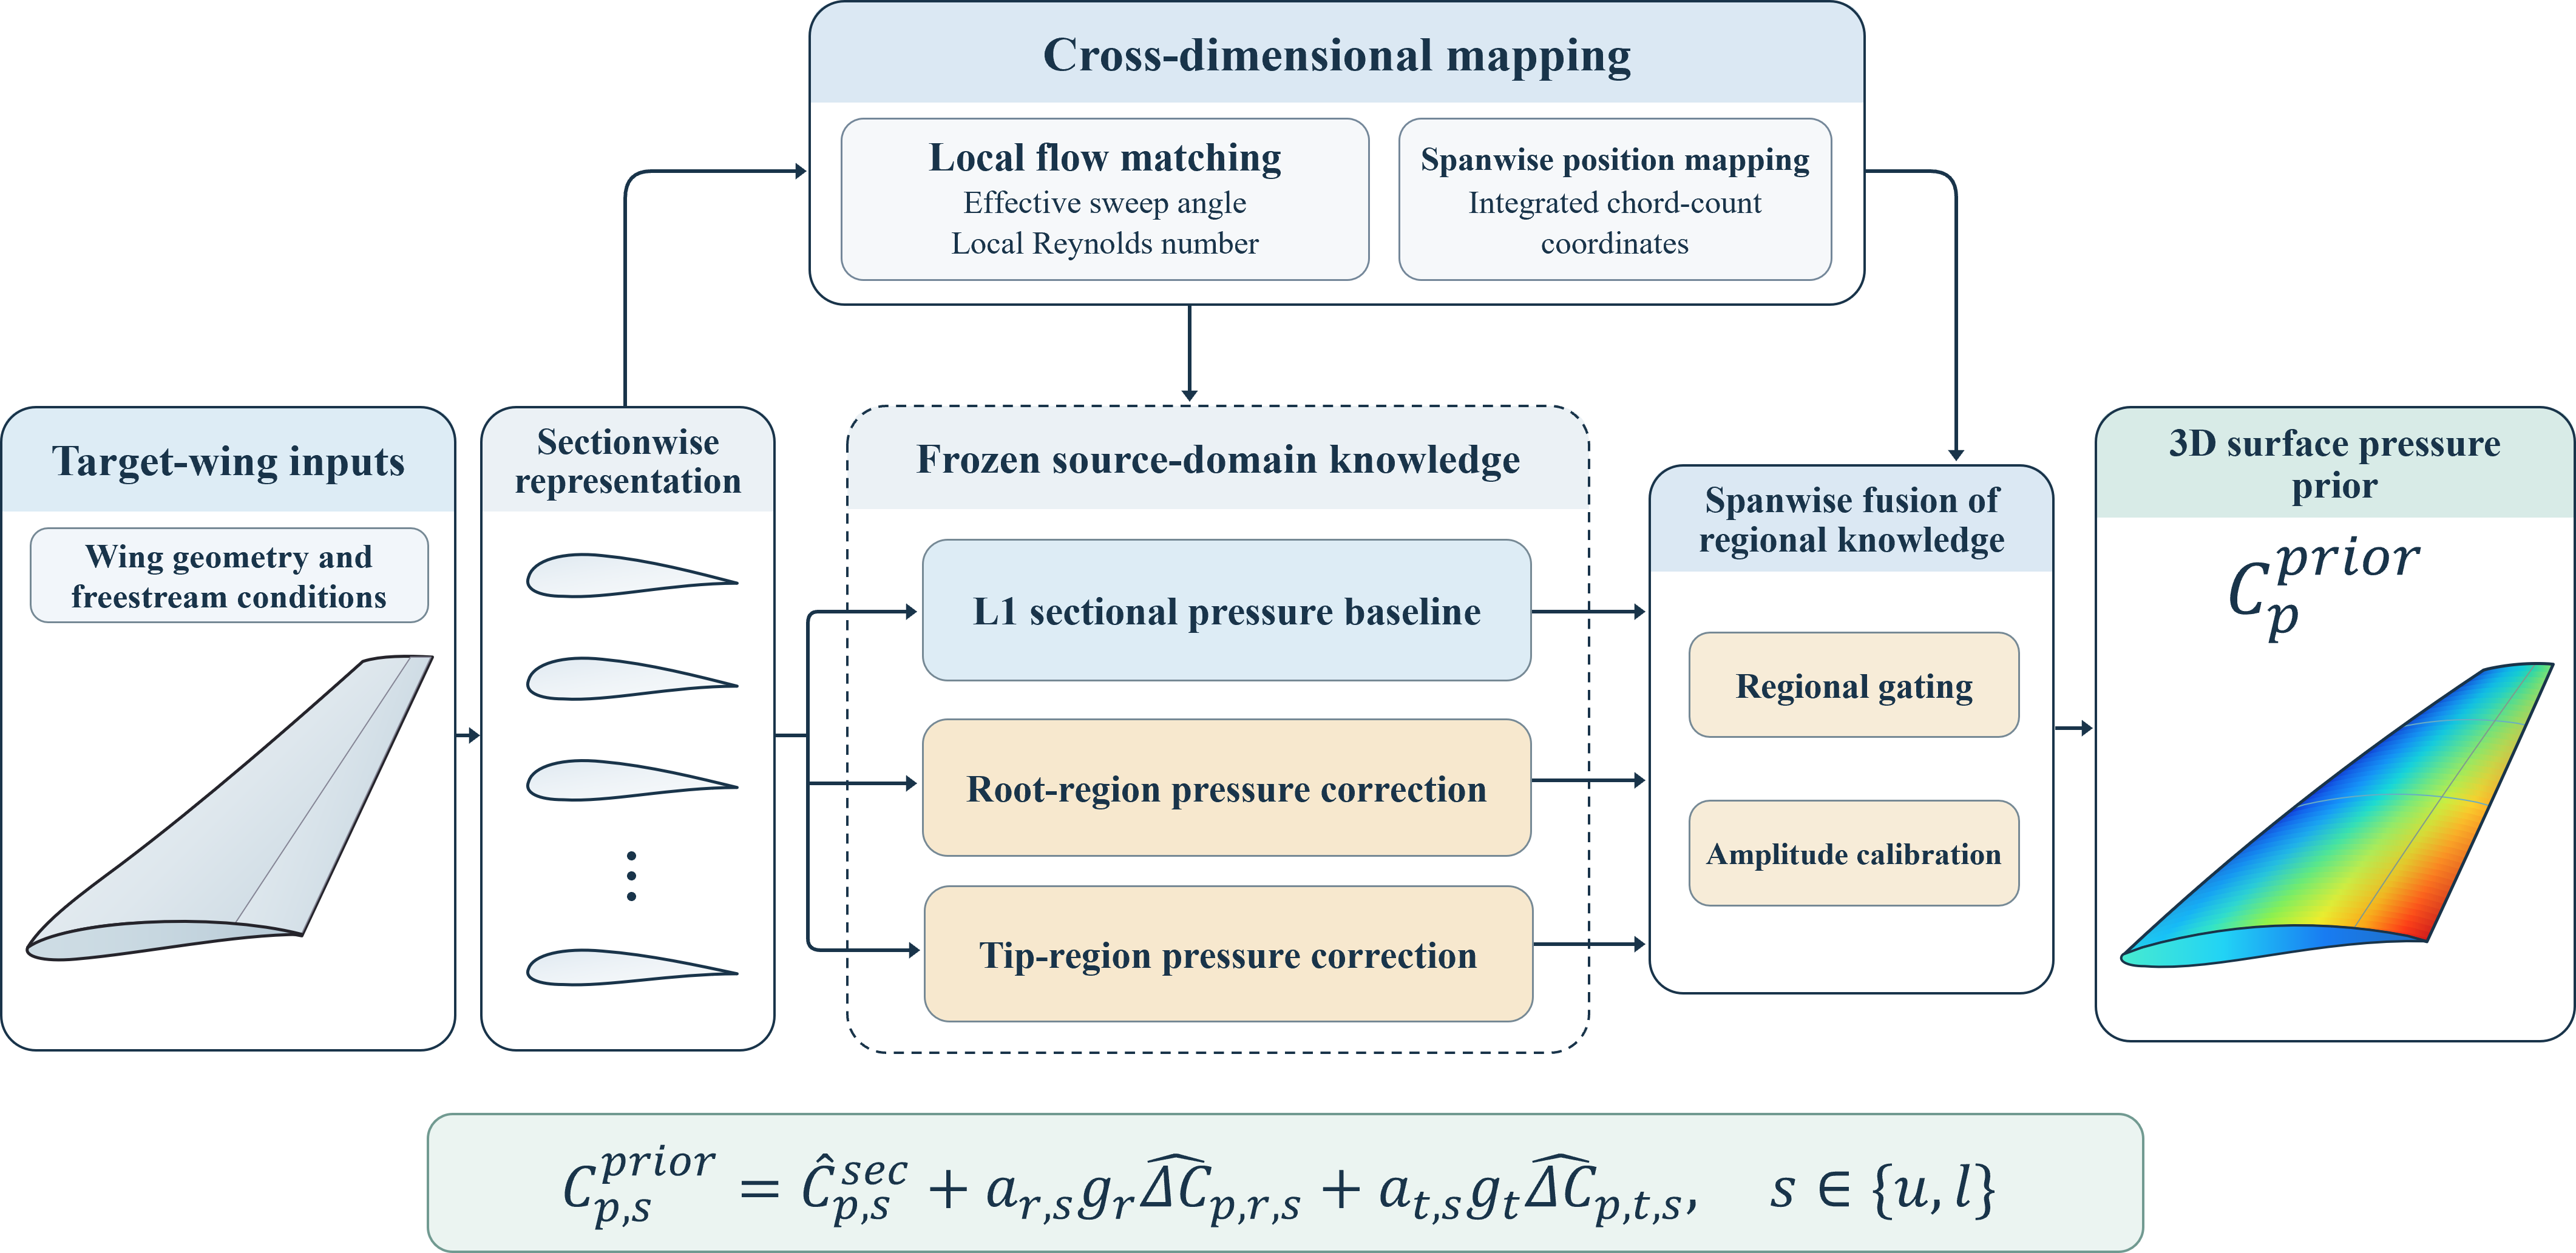
\includegraphics[width=0.98\textwidth]{III_Knowledge_Transfer/figures/III_C_Fig11/III_C_Fig11_hierarchical_prior_construction.png}
    \caption{Cross-dimensional knowledge projection and hierarchical pressure-prior construction for target-wing surface-pressure prediction.}
    \label{fig:hierarchical-prior-construction}
\end{figure*}



% D. Target-Domain Residual Pressure Prediction

% III.D. Target-Domain Residual Pressure Prediction

\subsection{Target-Domain Residual Pressure Prediction}
\label{sec:target-residual}

The hierarchical pressure prior developed in Sec.~\ref{sec:knowledge-projection} captures the sectional aerodynamic response and the transferred finite-span corrections, but does not fully resolve the three-dimensional pressure variations of the target configuration. The remaining discrepancy is defined as
\begin{equation}
R_{p,s}^{\mathrm{tar}}(\eta,\xi)
=
C_{p,s}^{3D,\mathrm{CFD}}(\eta,\xi)
-
C_{p,s}^{\mathrm{prior}}(\eta,\xi),
\quad s\in\{u,l\},
\label{eq:target-residual-definition}
\end{equation}
where $\eta$ and $\xi$ denote the normalized spanwise and chordwise coordinates, respectively. Rather than reconstructing the entire pressure field from target-domain samples, the residual model learns the pressure variations not adequately represented by the transferred knowledge. At each forward pass, the pressure prior is recomputed using the current regional gating and amplitude parameters, ensuring consistency between the network input and the reconstructed pressure.

The target-domain network combines target-wing geometric and flow information, an explicit hierarchical pressure prior, and latent features extracted from the frozen sectional baseline model. The pressure prior provides an initial aerodynamic reference field incorporating the sectional baseline response and the transferred root- and tip-region corrections. It also serves as an explicit input to the residual network. The frozen L1 sectional features, extracted after global feature fusion in the sectional model, are introduced into the upper- and lower-surface streams through separate trainable adapters. Thus, the transferred knowledge contributes both an initial pressure estimate and a learned representation of sectional aerodynamic characteristics.

As illustrated in Fig.~\ref{fig:target-residual-architecture}, the residual network employs a partially shared dual-surface architecture. Separate local encoders first extract chordwise features from the upper and lower surfaces. The corresponding frozen sectional features are transformed through surface-specific trainable adapters and combined with the local representations. The resulting features are then processed by separate multiscale axial residual convolutional networks (ResCNNs) with surface-specific weights, followed by spanwise Transformers with shared weights. Although the Transformer parameters are shared, the upper- and lower-surface features are processed separately. At each fixed chordwise location, the Transformers capture interactions among spanwise sections, using the normalized spanwise coordinate, local-to-root chord ratio, and root- and tip-based integrated chord counts as positional features.

Cross-surface coupling is subsequently introduced through an additional global spanwise interaction branch. This branch first pools the features of each surface along the chordwise direction, jointly processes the combined spanwise representations, and redistributes the resulting contextual information to the corresponding surface streams. This operation enables information exchange between the upper and lower surfaces while retaining their separate local feature representations. Independent residual heads then predict the pressure corrections for the two surfaces.

\begin{figure*}[t]
    \centering
    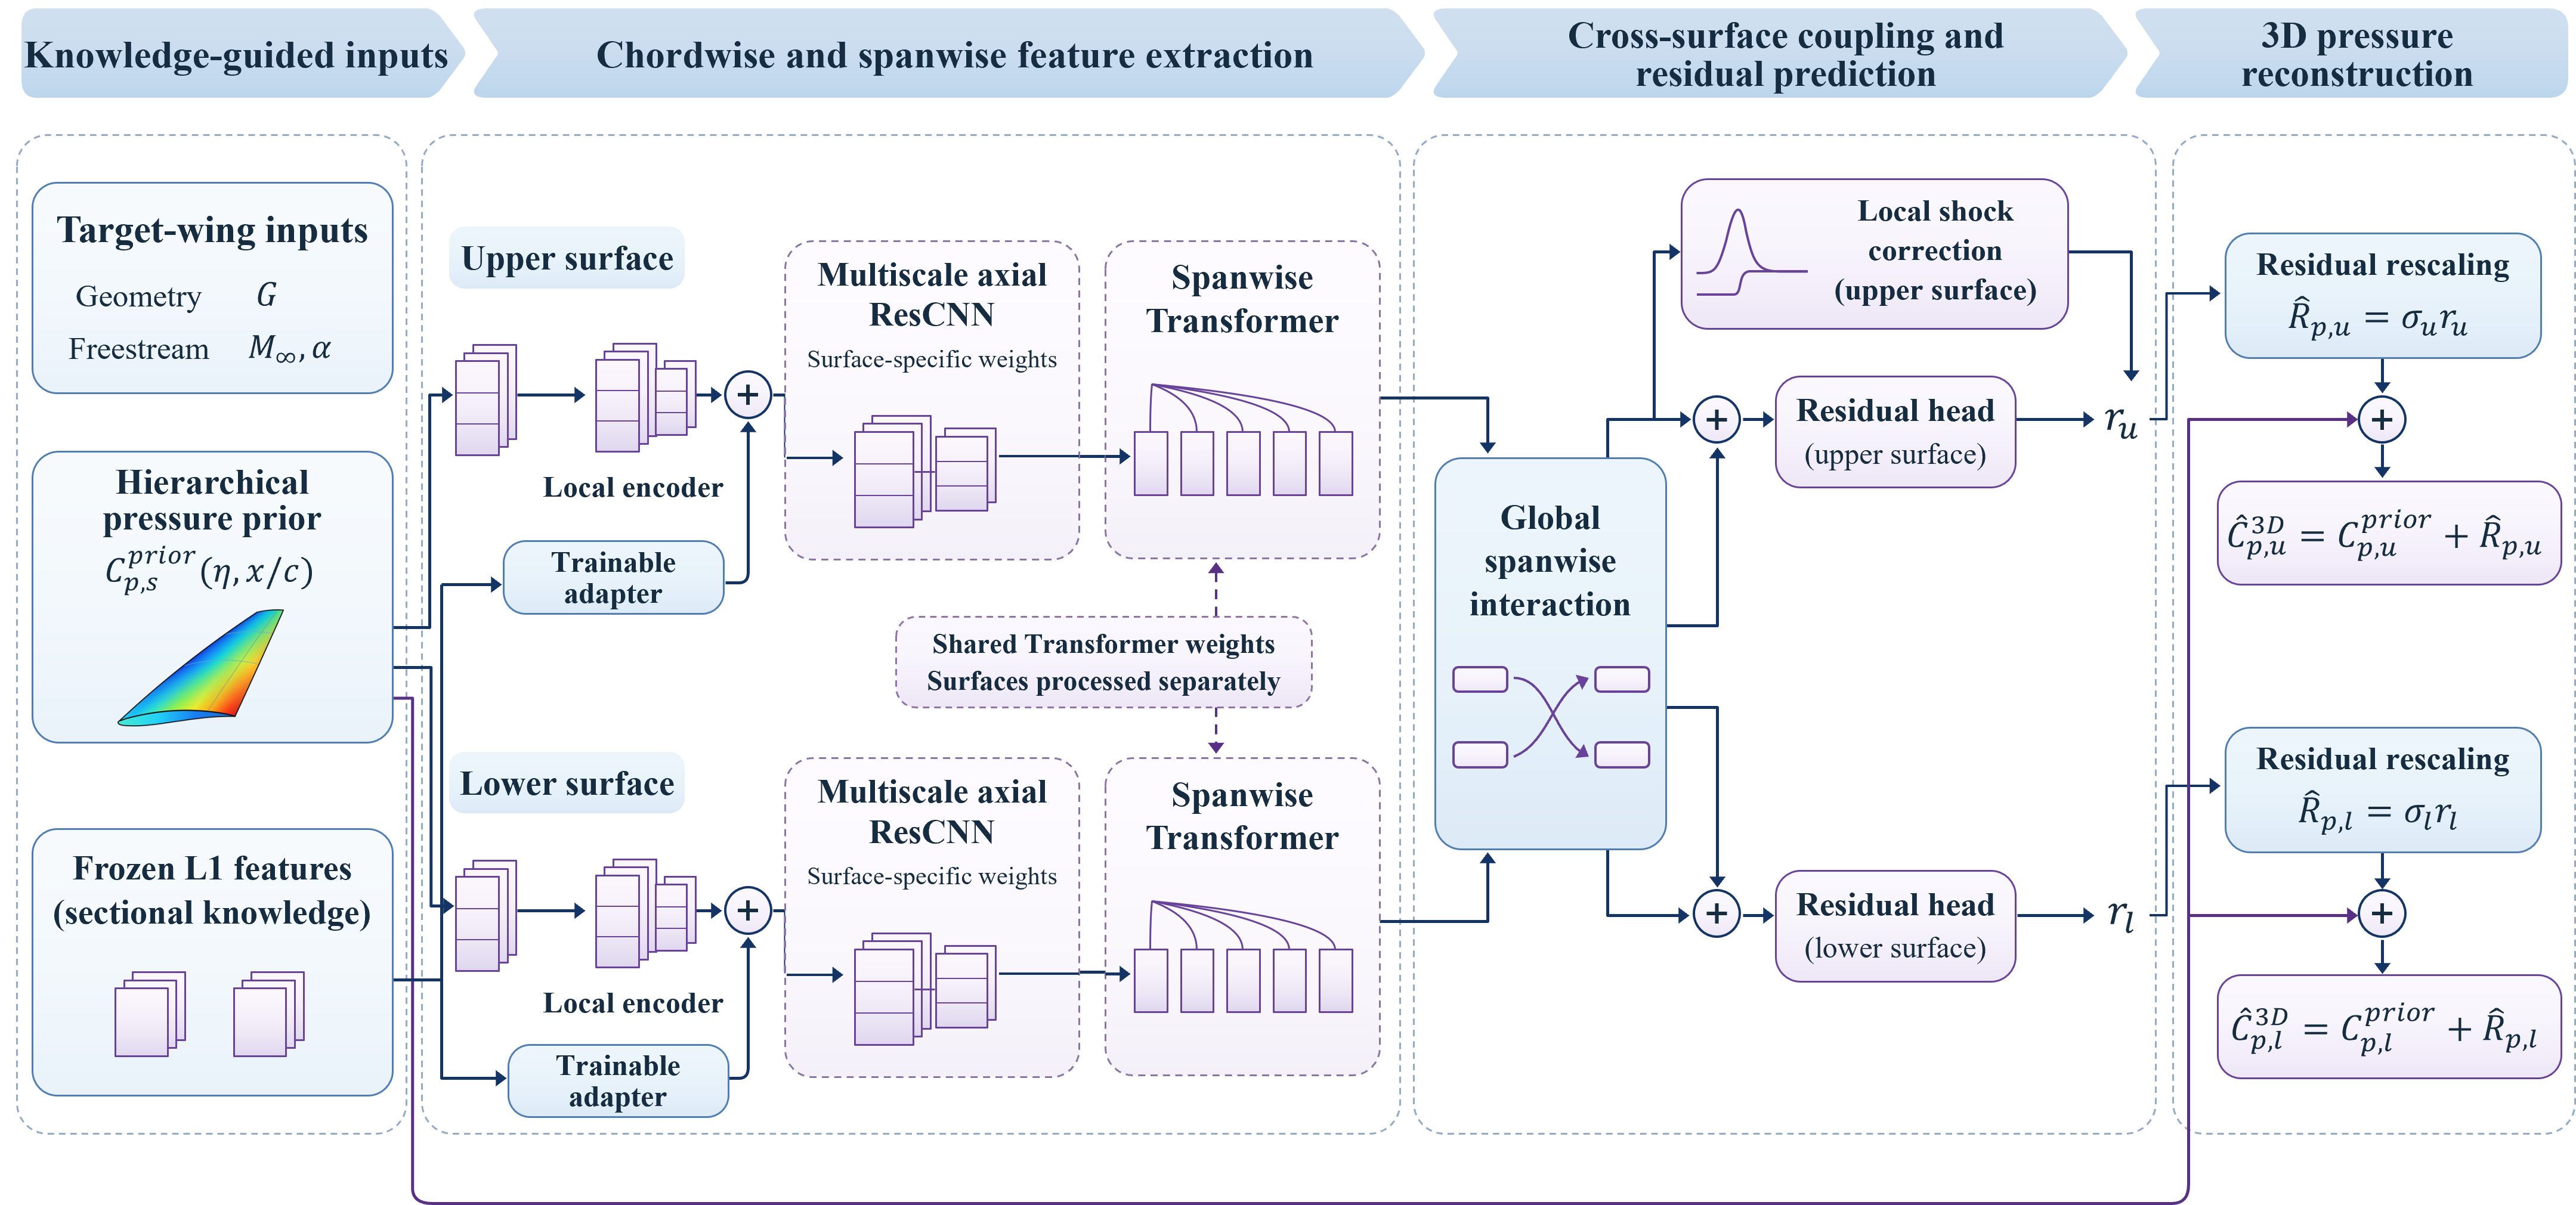
\includegraphics[width=0.98\textwidth]{III_Knowledge_Transfer/figures/III_D_Fig12/III_D_Fig12_target_residual_architecture.png}
    \caption{Architecture of the target-domain residual network}
    \label{fig:target-residual-architecture}
\end{figure*}

To provide an additional representation of abrupt pressure changes in transonic flow, a parametric shock-correction branch is applied to the upper surface. A reference location is estimated from the positive chordwise pressure gradient of the current pressure prior. Based on this reference, the network predicts a location shift, a characteristic width, a presence factor, and two correction amplitudes. The resulting parametric correction is added to the conventional upper-surface residual prediction, giving the standardized residual:
\begin{equation}
\begin{aligned}
r_u &= r_u^{\mathrm{head}}+p_{\mathrm{sh}}(A_G G+A_S S),\\
G &= \exp\left[-\frac{1}{2}\left(\frac{d}{w}\right)^2\right],\\
S &= \operatorname{sigmoid}\left(\frac{d}{w}\right).
\end{aligned}
\label{eq:upper-shock-correction}
\end{equation}

Here, $r_u^{\mathrm{head}}$ denotes the conventional upper-surface residual, and $d=\xi-\xi_{\mathrm{sh}}(\eta)$ is the distance from the predicted correction center. The parameters $w(\eta)$ and $p_{\mathrm{sh}}(\eta)$ represent the correction width and shock-presence factor, respectively, while $A_G(\eta)$ and $A_S(\eta)$ control the amplitudes of the Gaussian and sigmoid components. The dependence of $r_u$, $G$, and $S$ on $(\eta,\xi)$ is omitted for brevity. The correction center and presence logit receive explicit auxiliary supervision from target-domain CFD, whereas the width and amplitude parameters are learned through the reconstructed pressure.

The standardized residuals are converted into physical pressure-coefficient increments using surface-specific, zero-centered residual root-mean-square (RMS) scales computed from the target-domain training samples. The final prediction is
\begin{equation}
\widehat C_{p,s}^{3D}(\eta,\xi)
=
C_{p,s}^{\mathrm{prior}}(\eta,\xi)
+
\sigma_s r_s(\eta,\xi),
\quad s\in\{u,l\},
\label{eq:target-pressure-reconstruction}
\end{equation}
where $\sigma_s$ denotes the training-derived residual RMS scale for surface $s$. Zero initialization of the residual output heads and the shock-correction amplitude channels makes the initial prediction identical to the hierarchical pressure prior. The physical residual is subsequently learned without a final hyperbolic-tangent amplitude restriction.

The primary training objective is the pointwise mean squared error of the reconstructed pressure coefficients. Let $\mathcal V$ denote the set of valid surface nodes over the training batch, excluding the first chordwise node on each surface and the topologically degenerate exact tip section. The pressure loss is defined as
\begin{equation}
\mathcal L_{C_p}
=
\frac{1}{|\mathcal V|}
\sum_{(j,s,i)\in\mathcal V}
\left(
\widehat C_{p,s}^{3D,j}(\xi_i)
-
C_{p,s}^{3D,\mathrm{CFD},j}(\xi_i)
\right)^2,
\label{eq:target-pressure-mse}
\end{equation}
where $j$, $s$, and $i$ index the spanwise section, surface, and chordwise node, respectively. This normalization assigns equal weight to each valid pressure node, rather than assigning equal weight to the upper- and lower-surface mean squared errors.

Although the pointwise pressure loss constrains the reconstructed field, it does not explicitly distinguish the location, magnitude, or occurrence of localized pressure rises. Three auxiliary terms are therefore introduced for the upper surface. Reference features are derived from the positive chordwise pressure gradients of the CFD training labels at interval midpoints
\begin{equation*}
\bar{\xi}_i=\frac{\xi_i+\xi_{i+1}}{2},
\qquad 0.08\leq\bar{\xi}_i\leq0.85.
\end{equation*}
A section is considered to exhibit a pronounced pressure rise when its maximum positive gradient is at least 3.0. A softmax-weighted gradient centroid provides the reference location, while a similarly weighted sum of positive adjacent-node pressure increments characterizes the local pressure-rise magnitude. Both sets of gradient weights use the CFD reference peak, bounded below by 3.0, for normalization and a softmax temperature of 8.0. The latter descriptor is not a direct measure of the total shock pressure jump.

The location term applies a Smooth-$L_1$ penalty to the shock-correction center predicted by the network, using a chordwise normalization scale of 0.10. The magnitude term compares the pressure-rise descriptors evaluated from the final reconstructed and CFD pressure fields, normalized by the reference magnitude with a lower bound of 0.05. These two terms are computed only for sections with a detected pressure rise. In contrast, the presence term uses binary cross-entropy with logits for all valid sections, including those without a detected pressure rise. If no section is detected, the location and magnitude terms are set to zero.

The resulting training objective is
\begin{equation}
\begin{aligned}
\mathcal L={}&
\mathcal L_{C_p}
+\lambda_{\mathrm{pos}}\mathcal L_{\mathrm{pos}}\\
&+\lambda_{\mathrm{str}}\mathcal L_{\mathrm{str}}
+\lambda_{\mathrm{pres}}\mathcal L_{\mathrm{pres}},
\end{aligned}
\label{eq:target-total-loss}
\end{equation}
where $\mathcal L_{\mathrm{pos}}$, $\mathcal L_{\mathrm{str}}$, and $\mathcal L_{\mathrm{pres}}$ denote the location, pressure-rise magnitude, and presence losses, respectively. Their weights are fixed at
\begin{equation*}
\lambda_{\mathrm{pos}}=2\times10^{-4},
\qquad
\lambda_{\mathrm{str}}=10^{-4},
\qquad
\lambda_{\mathrm{pres}}=5\times10^{-5}
\end{equation*}
throughout training. The reference features and presence labels are computed from CFD data for training only; no reference pressure or CFD-based detection is required at inference.







% ===================================================
% IV. Experimental Design
% ===================================================

\section{Experimental Design}
\label{sec:experimental-design}

% A. Target-Domain Data Partition

\subsection{Target-Domain Data Partition and Few-Shot Learning Protocol}
\label{subsec:target-domain-protocol}

The target-domain database initially comprises 500 three-dimensional wing configurations with varying planforms. The initial training, validation, and test partitions contain 350, 50, and 100 configurations, respectively. Following mesh-validity and convergence screening, 437 configurations are retained, including 308 training candidates, 41 validation wings, and 88 test wings. The original assignments are preserved, and the three partitions are disjoint at the wing-configuration level. The validation set is used for model selection, whereas the test set provides a common basis for evaluating the selected models.

For surface-pressure prediction, seven target-domain training budgets are considered, $N\in\{10,20,30,40,50,80,100\}$. At each budget, the corresponding number of wings is selected from the 308 training candidates. A stratified, centroid-initialized maximin sampling strategy is employed based on flow conditions, planform parameters, and principal-component representations of airfoil geometry to improve the coverage of the design space. The principal training subsets are nested across budgets, such that smaller subsets are contained within larger ones. M0, M1, and M2 use matched wing selections at each budget to ensure a consistent comparison. Three independent training runs are conducted for each configuration to characterize run-to-run variability. In addition, the influence of training-set composition is examined separately at $N=20$ and $N=50$ using five alternative wing subsets, with the training random seed held fixed. Pressure-model checkpoints are selected based on their performance on the 41 validation wings. The common 88-wing test partition is excluded from training and checkpoint selection in the reported experiments and is used only to evaluate the frozen pressure models.

The aerodynamic-coefficient study uses the same seven budgets but follows a separate force-label protocol. At each budget, three independently sampled, nested training-subset sequences are constructed. Within each sequence, the direct regression model D0, the regression model D1 using M2-predicted pressure, and the regression model D2 using CFD-reference pressure are trained on matched wings. Separate regressors are fitted for the lift coefficient $C_L$, drag coefficient $C_D$, and pitching-moment coefficient $C_{M_z}$. The M2 pressure model used in D1 remains fixed; consequently, $N$ counts only the force-labeled target wings used for downstream regression, not the pressure data used to establish M2. All coefficient models are evaluated on the same 88 test wings. Error metrics are computed separately for each trained model before aggregation across the three training subsets, so repeated predictions of a test wing are not treated as additional independent test configurations.

The hierarchical aerodynamic knowledge models are trained according to their respective data dependencies. The sectional baseline pressure model is trained using the infinite-span swept-wing database, while the root- and tip-region correction models are trained separately using paired finite-span and infinite-span CFD data. These source-domain knowledge models remain frozen during subsequent target-domain training. The target-domain pressure models M0, M1, and M2, as well as the aerodynamic-coefficient regression models D0, D1, and D2, are trained using their corresponding target-domain training samples. All models employ the AdamW optimizer with an initial learning rate of $1\times10^{-3}$. The specific training configurations are summarized in Table~\ref{tab:training-configurations}.

\begin{table}[htbp]
    \centering
    \caption{Training configurations of the aerodynamic models}
    \label{tab:training-configurations}
    \small
    \setlength{\tabcolsep}{5pt}
    \renewcommand{\arraystretch}{1.15}
    \begin{tabular}{@{}lcccc@{}}
        \hline
        Model & Initial LR & Weight decay & Batch size & Epochs \\
        \hline
        Sectional baseline
        & $1\times10^{-3}$ & $1\times10^{-4}$ & 128 & 2000 \\

        Root/tip correction
        & $1\times10^{-3}$ & $1.5\times10^{-4}$ & 64 & 900 \\

        Target pressure (M0/M1/M2)
        & $1\times10^{-3}$ & $3\times10^{-4}$ & 2 & 600 \\

        Coefficient regression (D0/D1/D2)
        & $1\times10^{-3}$ & $1\times10^{-3}$ & 16 & 600 \\
        \hline
    \end{tabular}
\end{table}

For target-domain pressure models incorporating regional corrections, the gating parameters and correction amplitudes are initialized using the corresponding target-domain training samples and held fixed during the first 50 epochs. They are subsequently optimized jointly with the residual network, using an initial learning rate one-tenth that of the residual backbone. All source-domain knowledge models remain frozen throughout target-domain training. The root- and tip-region correction models and target-domain pressure models use validation-selected checkpoints, whereas the sectional baseline model uses its final trained parameters and the coefficient regressors use their final checkpoints determined by the training-error-based stopping criterion. The M2 pressure model used for aerodynamic-coefficient prediction is trained using 20 high-fidelity target-domain pressure samples and remains fixed across all downstream regression experiments.


% B. Comparative Models and Regional Knowledge Ablations

\subsection{Comparative Models and Regional Knowledge Ablations}
\label{subsec:comparative-models}

Three models, denoted as M0, M1, and M2, are considered for three-dimensional surface-pressure prediction. M0 uses only target-domain training data without incorporating pretrained aerodynamic knowledge. M1 introduces the sectional pressure prior and frozen features obtained from the infinite-span swept-wing model into the same three-dimensional prediction backbone. M2 further incorporates the wing-root and wing-tip pressure corrections and learns the target-domain residual relative to the complete hierarchical pressure prior. The three models share the same three-dimensional prediction backbone and differ primarily in the pretrained knowledge inputs and activated knowledge branches. The comparison between M0 and M1 evaluates the contribution of sectional knowledge transfer, whereas the comparison between M1 and M2 assesses the additional effect of regional pressure corrections.

To examine the separate contributions of wing-root and wing-tip knowledge, two additional ablation models, denoted as AR and AT, are considered at $N=20$. AR retains the sectional knowledge and wing-root pressure correction while disabling the wing-tip knowledge branch. Conversely, AT retains the sectional knowledge and wing-tip pressure correction while disabling the wing-root branch. For each ablation model, the pressure prior is recalibrated according to the activated knowledge components, and the target-domain prediction network is trained independently rather than disabling the corresponding branch of an already trained M2 model. The overall and spanwise regional pressure-prediction errors of M1, AR, AT, and M2 are compared to evaluate the individual and combined effects of the regional knowledge components.


% C. Pressure-Conditioned Aerodynamic Coefficient Prediction

\subsection{Pressure-Conditioned Aerodynamic Coefficient Prediction}
\label{subsec:force-coefficient-prediction}

The transfer of surface-pressure information to integrated aerodynamic prediction is investigated using separate single-output regressors for the lift coefficient $C_L$, drag coefficient $C_D$, and pitching-moment coefficient $C_{M_z}$. Each regressor maps geometric and flow-condition descriptors, together with a surface-pressure representation when available, to the corresponding CFD coefficient. The coefficients are learned directly from the force and moment labels rather than obtained by integrating the predicted pressure distribution.

Three input configurations are considered to distinguish the contribution of pressure information from its prediction accuracy. D0 performs direct regression using geometry and flow conditions alone. D1 additionally incorporates the surface-pressure distribution predicted by the pretrained M2 model, whose parameters remain fixed throughout coefficient-regressor training. D2 uses the corresponding CFD-reference pressure in place of the M2 prediction, providing a diagnostic reference for the value of more accurate pressure information. The regressors are fitted independently for each coefficient; D1 and D2 differ in the source of their pressure inputs, whereas D0 does not require a pressure input. The data-partition and repeated-sampling protocols are specified in Sec.~\ref{subsec:target-domain-protocol}.



% D. Training-Subset Sensitivity and Regional Evaluation

\subsection{Training-Subset Sensitivity and Regional Evaluation}
\label{subsec:training-subset-sensitivity-protocol}

To examine the influence of training-subset selection on pressure prediction, five alternative training subsets are considered at each of the two target-domain budgets, $N=20$ and $N=50$. Within each subset, M0, M1, and M2 use matched wing configurations, with the training random seed fixed at 3407 and all other settings following the baseline protocol. Each model is evaluated on the same 41 validation wings. The five subsets are not required to be mutually disjoint, and their results are used to assess the sensitivity of prediction performance to training-subset selection rather than treated as independent test-set realizations.

To evaluate regional error changes across the wing, saved predictions from three training seeds (3407, 3408, and 3409) are analyzed at $N=10$, 20, 50, and 100. Regional pressure RMSE is calculated for each validation wing using consistent valid-node masks and region definitions. Paired error differences are computed as M1 minus M0 and M2 minus M1 for the same wing, training budget, and random seed, with negative values indicating error reductions after introducing the corresponding knowledge components. The regional results are summarized using the mean paired error changes and the fractions of validation wings exhibiting positive error changes, aggregated across the three training seeds.








% ==================================================
% V. Results and Discussion
% ==================================================

\section{Results and Discussion}
\label{sec:results-and-discussion}

% A. Data Efficiency

\subsection{Data Efficiency of Hierarchical Knowledge Transfer}
\label{subsec:data-efficiency}

Figure~\ref{fig:cp-label-efficiency} presents the surface-pressure prediction errors of M0, M1, and M2 on 88 test wings under different target-domain training budgets. Both RMSE and MAE decrease with increasing training size, while the three knowledge configurations exhibit a consistent performance hierarchy. Incorporating sectional aerodynamic knowledge enables M1 to outperform the target-only baseline M0 across all training budgets. With the additional wing-root and wing-tip corrections, M2 further improves prediction accuracy. These results indicate that transferable sectional knowledge provides an effective basis for wing pressure prediction, while regional aerodynamic knowledge offers additional information for representing three-dimensional pressure variations.

\begin{figure*}[!t]
    \centering
    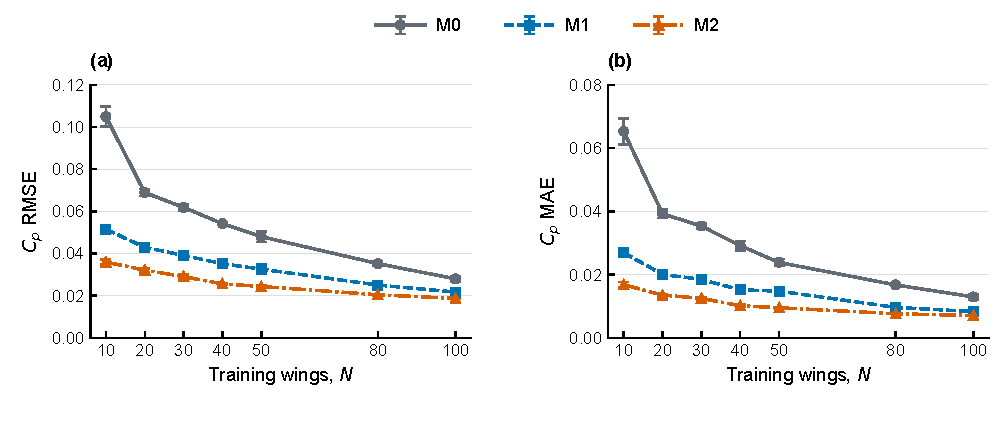
\includegraphics[width=0.90\textwidth]{V_Results_and_Discussion/figures/V_A_Fig13/V_A_Fig13_cp_label_efficiency.pdf}
    \caption{urface-pressure prediction errors at different training sizes: (a) RMSE and (b) MAE. Results are evaluated on 88 test wings over three runs.}
    \label{fig:cp-label-efficiency}
\end{figure*}


The benefit of hierarchical knowledge transfer is particularly evident under limited target-domain supervision. At $N=10$, M2 achieves an RMSE of 0.03593, corresponding to a mean reduction of 65.74\% relative to M0, as summarized in Table~\ref{tab:cp-data-efficiency}. Although the relative improvement from hierarchical knowledge transfer decreases as the target-domain training size increases, M2 consistently achieves the lowest prediction error across all training budgets. This indicates that sectional aerodynamic knowledge and regional corrections provide complementary information for target-domain pressure prediction across different data regimes, with particularly pronounced benefits when only limited target-domain samples are available.

\begin{table*}[!t]
    \centering
    \caption{Surface-pressure RMSE on 88 test wings at representative training sizes.}
    \label{tab:cp-data-efficiency}
    \small
    \renewcommand{\arraystretch}{1.15}
    \begin{tabular}{ccccc}
        \hline
        Training wings $N$ & M0 & M1 & M2 & M2 vs. M0 (\%) \\
        \hline
        10  & $0.10493 \pm 0.00470$ & $0.05150 \pm 0.00072$ & $0.03593 \pm 0.00117$ & 65.74 \\
        20  & $0.06893 \pm 0.00164$ & $0.04293 \pm 0.00094$ & $0.03210 \pm 0.00077$ & 53.43 \\
        50  & $0.04797 \pm 0.00250$ & $0.03258 \pm 0.00210$ & $0.02434 \pm 0.00079$ & 49.15 \\
        100 & $0.02796 \pm 0.00117$ & $0.02170 \pm 0.00157$ & $0.01869 \pm 0.00034$ & 33.04 \\
        \hline
    \end{tabular}
\end{table*}


% B. Regional Aerodynamic Knowledge

\subsection{Contributions and Spatial Effects of Regional Aerodynamic Knowledge}
\label{sec:regional_knowledge_contributions}

The contribution of transferred aerodynamic knowledge is not uniform along the wing span. Figure~\ref{fig:vb_spanwise} compares the sectional pressure-prediction errors of M0, M1, and M2 at three target-domain training sizes. Relative to direct three-dimensional learning (M0), sectional knowledge transfer (M1) reduces the errors over a broad spanwise range, whereas the additional gains from regional knowledge (M2) vary with spanwise position. The differences are particularly evident at $N=10$ and $20$, for which M2 yields lower mean sectional RMSE than M1 throughout the evaluated span on both surfaces. At $N=100$, the errors are considerably smaller and the two knowledge-based models approach one another, with limited local reversals in their relative performance. The larger upper-surface errors, especially toward the outboard wing, also indicate that the remaining prediction difficulty is spatially nonuniform. Thus, the additional value of regional knowledge depends on both spanwise location and the amount of target-domain supervision.

\begin{figure*}[t]
    \centering
    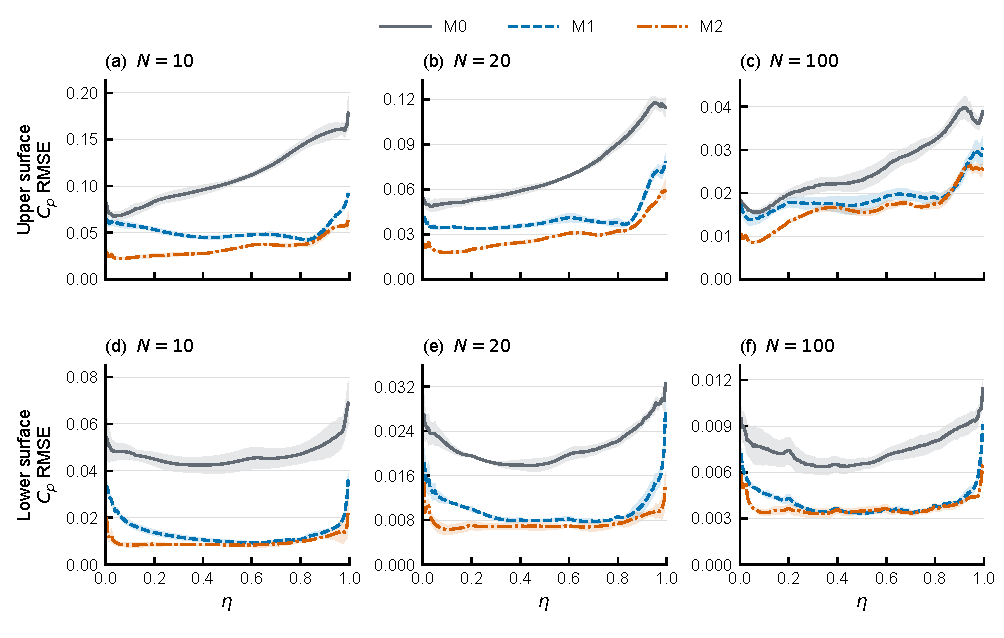
\includegraphics[width=\textwidth]{V_Results_and_Discussion/figures/V_B_Fig14/V_B_Fig14_vb_spanwise.pdf}
    \caption{Spanwise sectional RMSE of M0, M1, and M2 at three training sizes for both surfaces (88 test wings; mean $\pm$ standard deviation over three runs).}
    \label{fig:vb_spanwise}
\end{figure*}



The ablation results at $N=20$ clarify the distinct spatial contributions of the two regional knowledge components (Fig.~\ref{fig:vb_ablation}). Relative to M1, retaining only the wing-root correction (AR) reduces the root-region RMSE by $36.25\%$, but provides a much smaller improvement near the tip. In contrast, retaining only the wing-tip correction (AT) reduces the tip-region RMSE by $17.81\%$, while increasing the root-region error by $5.47\%$. These contrasting responses are consistent with the different spatial characteristics represented by the root and tip knowledge models. When both components are included, M2 attains the lowest mean RMSE among the four configurations in all three regions, with reductions of $39.81\%$, $24.69\%$, and $20.66\%$ relative to M1 in the root, midspan, and tip regions, respectively. The improvement in the midspan region indicates that the benefits of regional knowledge are not confined to the regions used to define the corrections. Nevertheless, the additional gain of M2 over the corresponding single-region model is comparatively modest, particularly near the tip, and is not reproduced in every training run. The combined prior therefore improves the regional averages without ensuring a uniform advantage at every location.

\begin{figure*}[t]
    \centering
    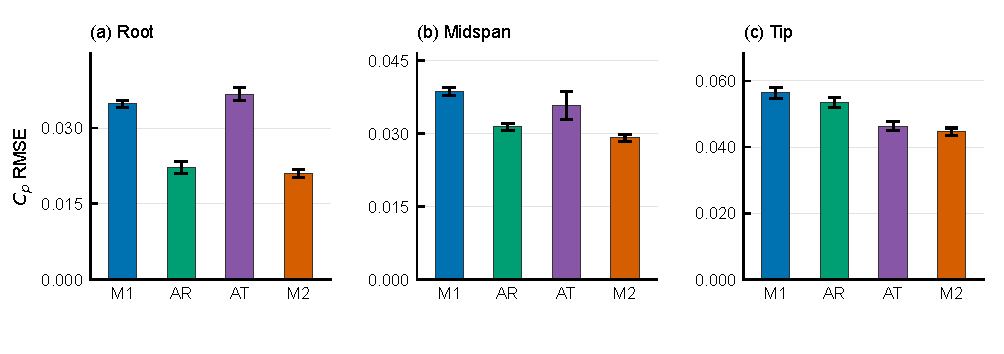
\includegraphics[width=\textwidth]{V_Results_and_Discussion/figures/V_B_Fig15/V_B_Fig15_vb_ablation.pdf}
    \caption{Regional pressure RMSE at $N=20$: (a) root, (b) midspan, and (c) tip.}
    \label{fig:vb_ablation}
\end{figure*}

The reconstruction of the chordwise pressure distributions provides a complementary view of these error statistics. Figure~\ref{fig:vb_cp_sections} shows ten spanwise sections of a test wing at $M_\infty=0.7836$ and $\alpha=3.512^\circ$, predicted by M2 at $N=20$. When the 88 test wings were ranked in ascending order of whole-wing $C_p$ RMSE averaged over the three M2 training runs, this wing ranked 54th. Across the span, M2 reproduces the main upper- and lower-surface pressure trends, including the suction distributions and subsequent pressure recovery. Agreement is closer at $\eta\approx0.755$ and $0.850$, whereas appreciable upper-surface discrepancies remain around $\eta\approx0.550$ and $0.655$. The combined sectional RMSE ranges from $0.01483$ to $0.04209$ among the ten displayed sections. The resulting variation shows that an accurate overall pressure reconstruction can coexist with localized errors in the chordwise loading distribution.

\begin{figure*}[t]
    \centering
    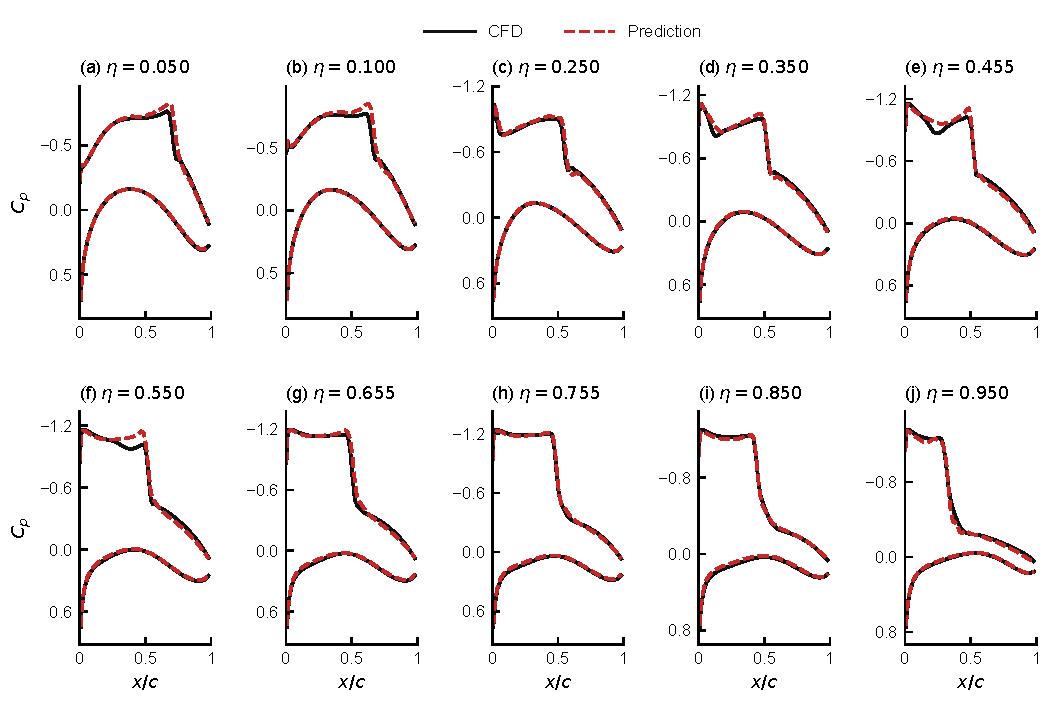
\includegraphics[width=\textwidth]{V_Results_and_Discussion/figures/V_B_Fig16/V_B_Fig16_vb_cp_sections.pdf}
    \caption{CFD and M2 pressure distributions at ten spanwise sections ($M_\infty=0.7836$, $\alpha=3.512^\circ$; $N=20$).}
    \label{fig:vb_cp_sections}
\end{figure*}

For the same test wing shown in Fig.~\ref{fig:vb_cp_sections}, the local pressure comparisons in Fig.~\ref{fig:vb_cp_regions} further show why regional-average improvements should not be interpreted as gains at every section. At the root section ($\eta\approx0.100$), AR reduces the lower-surface RMSE from $0.01151$ for M1 to $0.00343$, while the upper-surface RMSE increases slightly because of residual discrepancies in the aft-chord pressure recovery. Consequently, the combined sectional RMSE changes only marginally; M2 exhibits a larger upper-surface error at this particular section. A similar surface-dependent response occurs at the tip section ($\eta\approx0.950$). AT lowers the lower-surface RMSE from $0.01321$ to $0.00393$, but its upper-surface error increases, resulting in a higher combined sectional RMSE than M1. These case-specific deviations do not contradict the improvements observed over the 88-wing test set. Rather, they illustrate that regional knowledge contributes useful finite-wing pressure information whose effectiveness depends on the local pressure characteristics and its interaction with target-domain residual learning. Further improvement of the hierarchical framework therefore requires not only transferable regional corrections but also their appropriate combination across the wing surface.

\begin{figure*}[t]
    \centering
    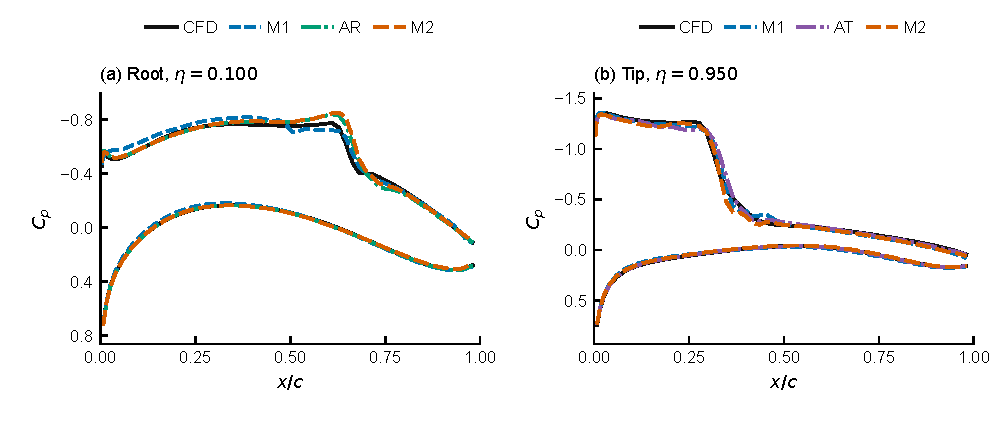
\includegraphics[width=\textwidth]{V_Results_and_Discussion/figures/V_B_Fig17/V_B_Fig17_vb_cp_regions.pdf}
    \caption{Local pressure distributions at the near-root ($\eta\approx0.100$) and near-tip ($\eta\approx0.950$) sections of the test wing in Fig.~\ref{fig:vb_cp_sections} ($N=20$).}
    \label{fig:vb_cp_regions}
\end{figure*}


% C. Three-Dimensional Pressure Prediction

\subsection{Three-Dimensional Pressure Prediction and Spatial Error Analysis}
\label{subsec:pressure-spatial-errors}


Figure~\ref{fig:cp-spatial-error-map} shows the spatial distribution of surface-pressure prediction errors at $N=20$, evaluated across the validation wings. For M0, relatively large errors are concentrated on the upper surface, particularly over the forward and midchord portions of the outboard wing. Introducing sectional pressure knowledge reduces these errors over a broad area, while M2 further suppresses several localized regions of high error. The lower-surface errors are generally smaller, consistent with the spanwise error distributions presented in Fig.~\ref{fig:vb_spanwise}. Nevertheless, appreciable errors remain in parts of the outboard upper surface even for M2, indicating that the improvement in pressure prediction is spatially nonuniform.


\begin{figure*}[!t]
    \centering
    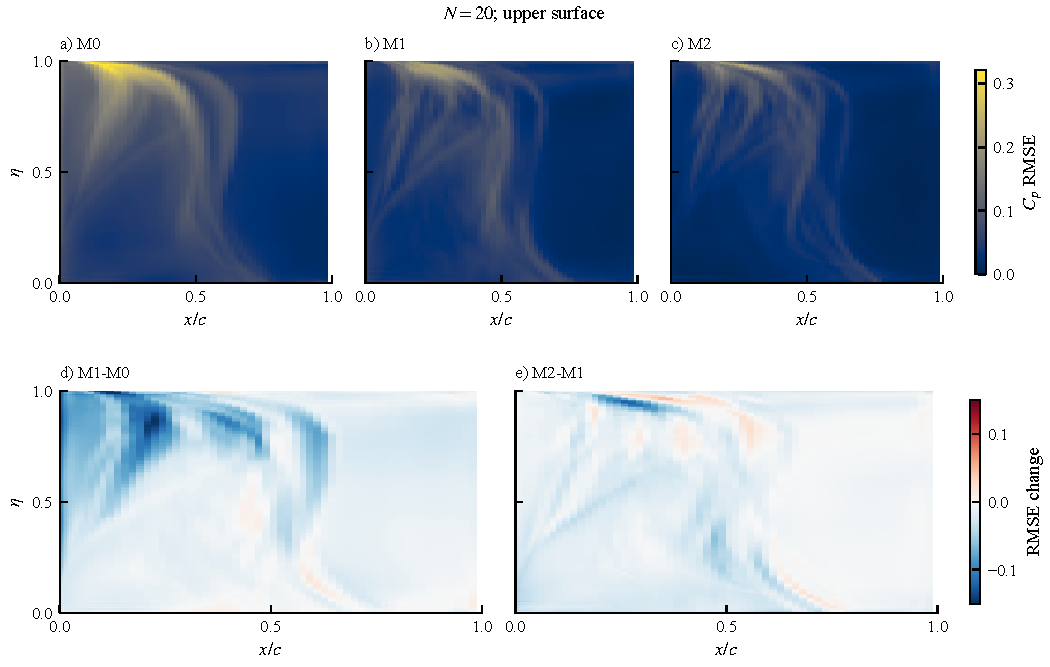
\includegraphics[width=0.93\textwidth]{V_Results_and_Discussion/figures/V_C_Fig18/V_C_Fig18_cp_spatial_error_map.pdf}
    \caption{Upper-surface RMSE maps and differences (M1$-$M0, M2$-$M1) at $N=20$ (41 validation wings; three-run mean). Negative differences indicate error reductions.}
    \label{fig:cp-spatial-error-map}
\end{figure*}

To examine the reconstruction of individual pressure fields, two validation wings with different baseline prediction difficulties are considered. Case A is selected near the median of the wingwise M0 error ranking. As shown in Figs.~\ref{fig:case-a-pressure-field} and \ref{fig:case-a-pressure-sections}, the three models broadly reproduce the spatial pattern of the reference pressure distribution, while M1 and M2 provide improved predictions relative to M0 in several regions of local pressure variation. The chordwise sections further show that the knowledge-based models generally capture the upper- and lower-surface pressure distributions more closely. However, the whole-wing errors of M1 and M2 remain comparable, illustrating that improvements at a small number of representative sections do not necessarily translate into a lower error over the entire wing surface.

\begin{figure*}[!t]
    \centering
    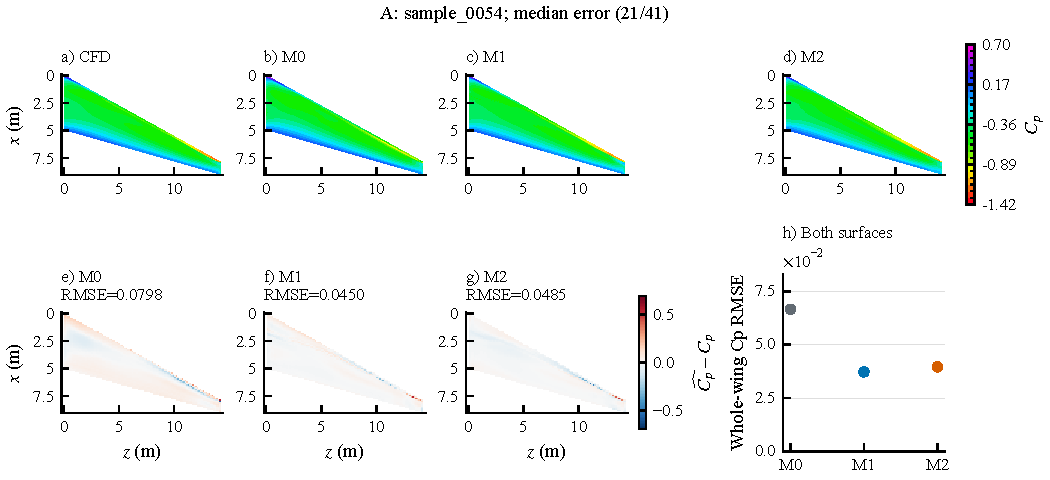
\includegraphics[width=0.93\textwidth]{V_Results_and_Discussion/figures/V_C_Fig19/V_C_Fig19_case_a_pressure_field.pdf}
    \caption{Upper-surface pressure and signed-error fields for Case A ($N=20$), selected near the median M0 RMSE.}
    \label{fig:case-a-pressure-field}
\end{figure*}

\begin{figure*}[!t]
    \centering
    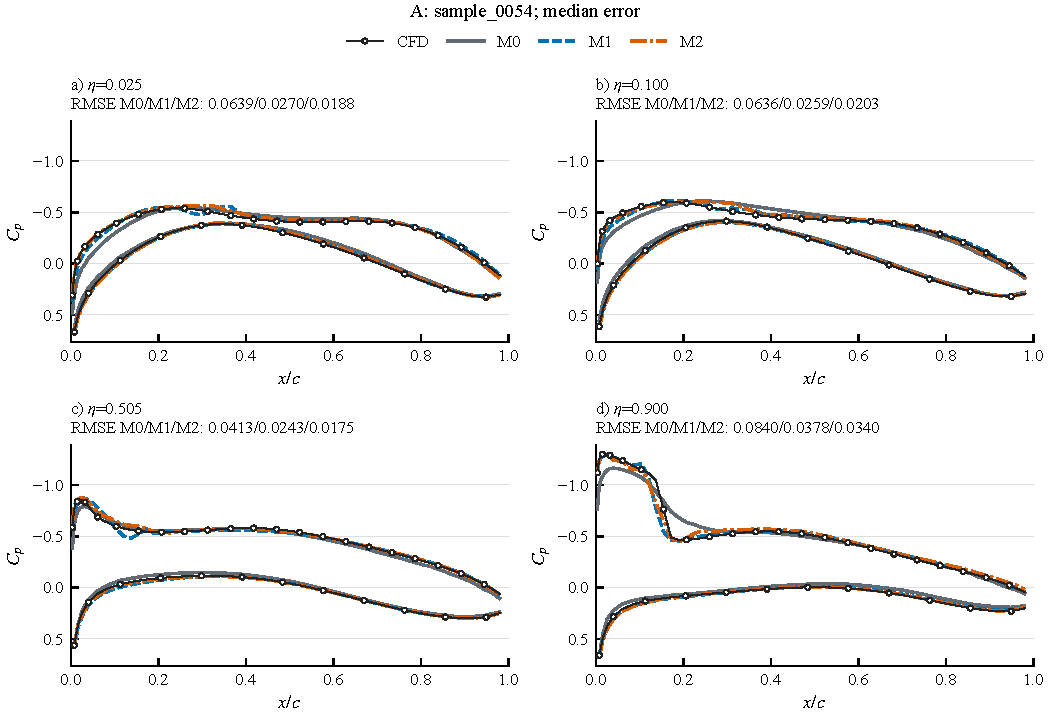
\includegraphics[width=0.93\textwidth]{V_Results_and_Discussion/figures/V_C_Fig20/V_C_Fig20_case_a_pressure_sections.pdf}
    \caption{Chordwise $C_p$ distributions for Case A at four spanwise stations ($N=20$).}
    \label{fig:case-a-pressure-sections}
\end{figure*}

The differences among the knowledge configurations are more pronounced for Case B, which is selected near the 90th percentile of the M0 wingwise error ranking. As shown in Figs.~\ref{fig:case-b-pressure-field} and \ref{fig:case-b-pressure-sections}, the upper-surface pressure distribution exhibits steep pressure recovery over portions of the midspan and outboard wing. M0 and M1 show noticeable discrepancies in the location and shape of these chordwise variations, whereas M2 more closely follows the reference distribution, particularly at outboard stations. At $\eta=0.90$, the sectional RMSE values of M0, M1, and M2 are 0.1520, 0.1476, and 0.0477, respectively. The corresponding whole-wing RMSE values are 0.1092, 0.1024, and 0.0503, demonstrating a substantial improvement in pressure reconstruction for this relatively difficult configuration.

\begin{figure*}[!t]
    \centering
    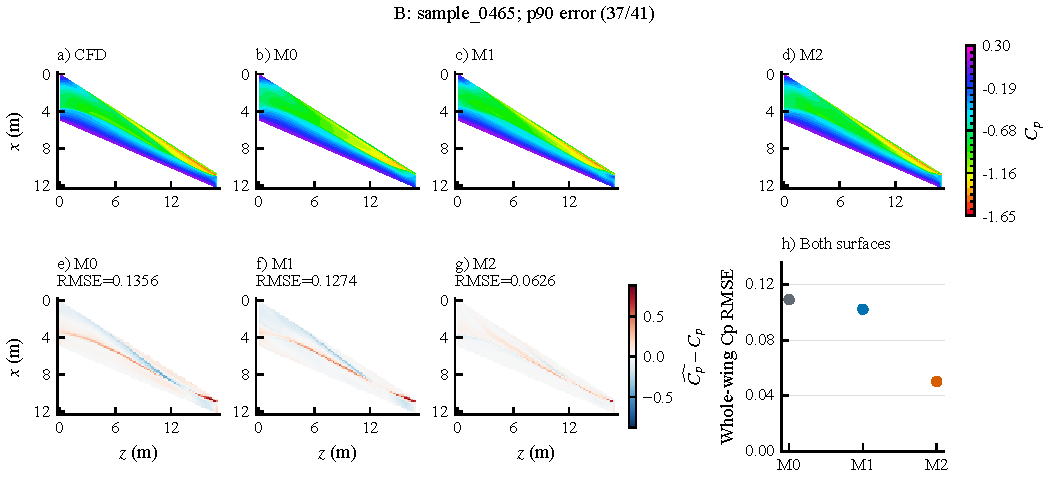
\includegraphics[width=0.93\textwidth]{V_Results_and_Discussion/figures/V_C_Fig21/V_C_Fig21_case_b_pressure_field.pdf}
    \caption{Upper-surface pressure and signed-error fields for Case B ($N=20$), selected near the 90th percentile of the M0 RMSE ranking.}
    \label{fig:case-b-pressure-field}
\end{figure*}

\begin{figure*}[!t]
    \centering
    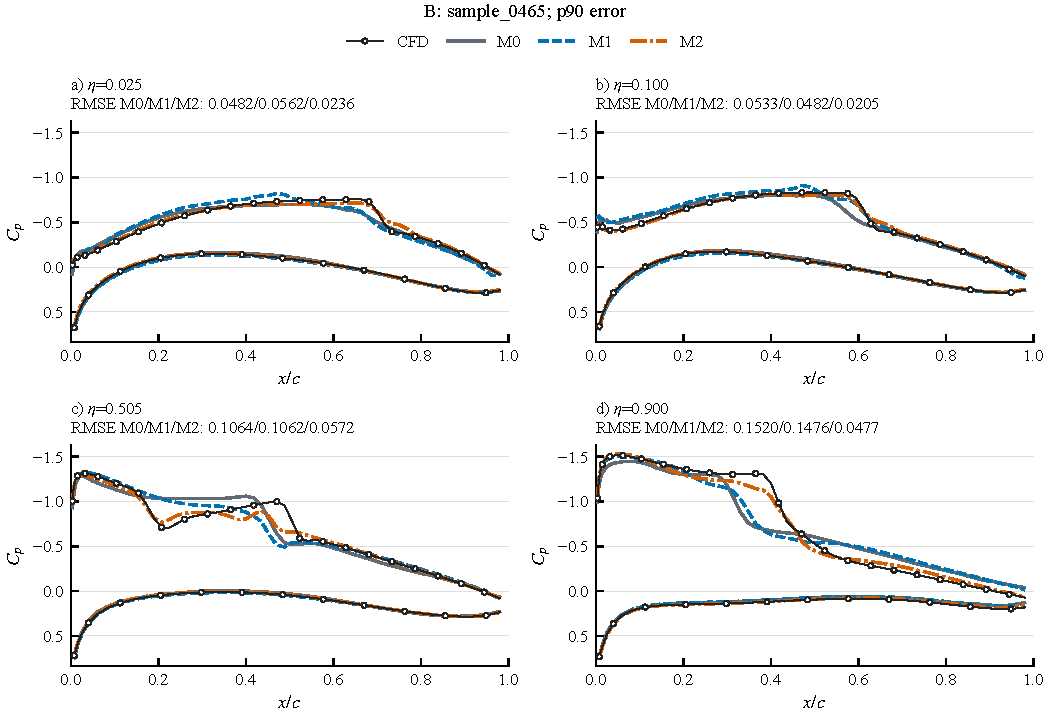
\includegraphics[width=0.93\textwidth]{V_Results_and_Discussion/figures/V_C_Fig22/V_C_Fig22_case_b_pressure_sections.pdf}
    \caption{Chordwise $C_p$ distributions for Case B at four spanwise stations ($N=20$).}
    \label{fig:case-b-pressure-sections}
\end{figure*}

Taken together, the spatial error statistics and representative cases show that hierarchical knowledge transfer improves not only the overall pressure-prediction accuracy but also the reconstruction of certain localized features associated with steep pressure gradients and rapid pressure recovery. The gains nevertheless depend on wing configuration and spanwise location, and noticeable discrepancies persist in some regions of strong pressure variation. The individual cases serve to illustrate these spatial characteristics, whereas conclusions about overall predictive performance are based on the validation-set statistics.



% D. Training-Subset Selection Sensitivity

\subsection{Sensitivity to Training-Subset Selection and Consistency of Regional Predictions}
\label{subsec:training-selection-sensitivity}

Under limited training data, prediction accuracy can be sensitive to the selection of target-domain samples. Figure~\ref{fig:training-selection-stability} compares the validation errors of M0, M1, and M2 across five different training subsets at $N=20$ and $N=50$. With the network training random seed held fixed, changing the training subset introduces variations in RMSE, while the relative performance of the three knowledge configurations remains consistent. M1 outperforms M0 across all examined subsets, and M2 consistently achieves the lowest errors. For M2, the RMSE ranges from 0.0312 to 0.0374 at $N=20$, narrowing to 0.0242--0.0259 at $N=50$. These results indicate that the accuracy advantage of hierarchical knowledge transfer is maintained across the examined training subsets rather than depending on a particular selection of target-domain samples.

\begin{figure*}[!t]
    \centering
    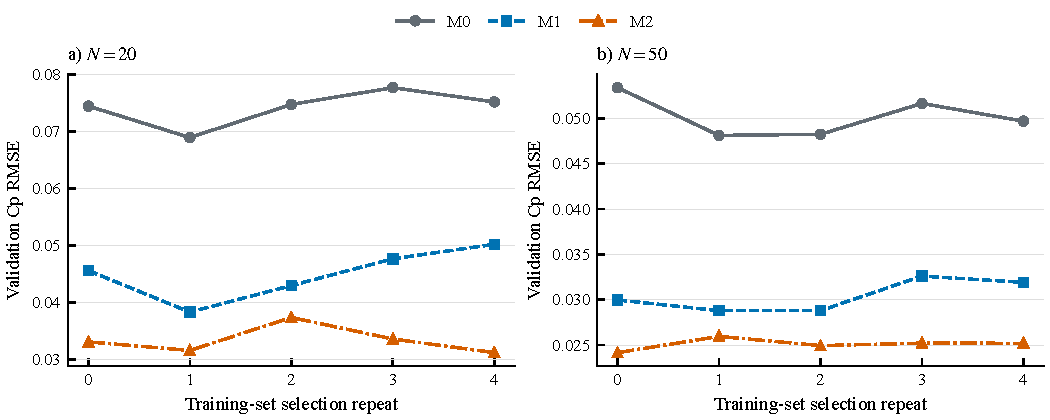
\includegraphics[width=0.93\textwidth]{V_Results_and_Discussion/figures/V_D_Fig23/V_D_Fig23_training_selection_stability.pdf}
    \caption{Training-subset sensitivity of M0, M1, and M2 at $N=20$ and $50$ .}
    \label{fig:training-selection-stability}
\end{figure*}

Although the overall prediction accuracy improves with transferred aerodynamic knowledge, the local benefits vary among individual validation wings. Figure~\ref{fig:regional-error-consistency} presents the mean changes in regional RMSE and the fractions of validation wings exhibiting increased errors at different training sizes. The improvement from M0 to M1 is observed for most validation wings in the midspan and wing-tip regions, while the additional improvement from M1 to M2 is more consistent near the wing root. At $N=10$ and $N=20$, only a small fraction of validation wings exhibit increased root-region errors, indicating that the benefits of wing-root knowledge extend beyond a reduction in the mean regional error.

\begin{figure*}[!t]
    \centering
    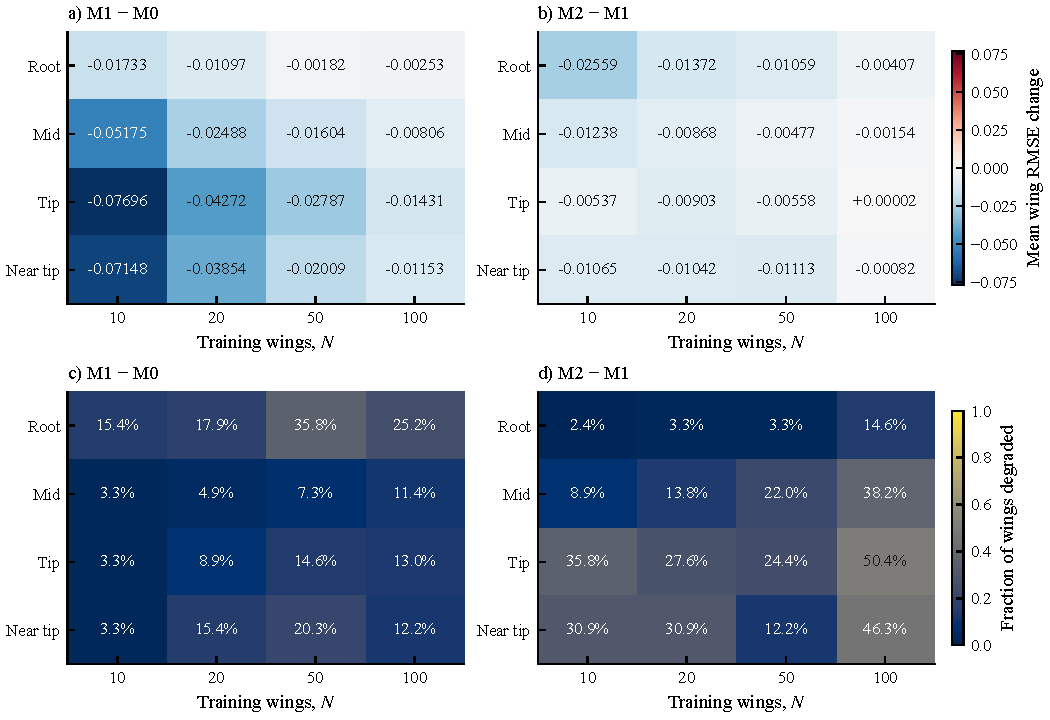
\includegraphics[width=0.95\textwidth]{V_Results_and_Discussion/figures/V_D_Fig24/V_D_Fig24_regional_error_consistency.pdf}
    \caption{Regional RMSE changes and error-increase fractions for M1$-$M0 and M2$-$M1 across four regions and training sizes.}
    \label{fig:regional-error-consistency}
\end{figure*}

As the number of target-domain training samples increases, both the additional benefits of regional knowledge and their consistency across validation wings change. At $N=100$, M2 retains a mean accuracy advantage over M1 in the wing-root region, whereas the additional improvements in the midspan and wing-tip regions become considerably smaller. In particular, the mean RMSE difference in the wing-tip region approaches zero. It should be noted that the fraction of wings exhibiting increased errors reflects only the direction of the paired error changes, rather than their magnitude. Small numerical differences should therefore not be interpreted as substantial prediction degradation. Overall, hierarchical knowledge transfer maintains its accuracy advantage across different training-subset selections, although the consistency of local improvements depends on spanwise location and the availability of target-domain training data.


% E. Aerodynamic Coefficient Prediction

% V_Results_and_Discussion/V_E_Force_Performance.tex
% English AIAA manuscript subsection
% Included by main.tex using:
% 
% V_Results_and_Discussion/V_E_Force_Performance.tex
% English AIAA manuscript subsection
% Included by main.tex using:
% 
% V_Results_and_Discussion/V_E_Force_Performance.tex
% English AIAA manuscript subsection
% Included by main.tex using:
% \input{V_Results_and_Discussion/V_E_Force_Performance}

\subsection{Aerodynamic Coefficient Prediction Performance}
\label{subsec:aerodynamic-coefficient-prediction}

Accurate reconstruction of the surface pressure field does not, by itself, guarantee accurate prediction of integrated aerodynamic coefficients. The latter requires a downstream model to extract the load-relevant information from a high-dimensional pressure representation. The force-label efficiency of this representation is examined using three coefficient-regression strategies: direct regression from geometry and flow conditions (D0), regression conditioned on the pressure field predicted by the fixed M2 model (D1), and regression conditioned on CFD-reference pressure (D2). Separate regressors are trained for the lift coefficient $C_L$, drag coefficient $C_D$, and pitching-moment coefficient $C_{M_z}$. Seven force-label budgets, $N=10$, 20, 30, 40, 50, 80, and 100 wings, are considered, with three independently sampled training subsets at each budget. All reported errors are evaluated on the same 88 test wings. Here $N$ denotes the number of wings used to train the downstream coefficient regressors; the pressure supervision previously used to establish the fixed M2 model is not included in this budget. Figure~\ref{fig:ve-force-mae} shows the mean absolute error (MAE) across the seven budgets, and Table~\ref{tab:ve-force-mae} provides the corresponding numerical comparisons.

\begin{figure*}[!t]
    \centering
    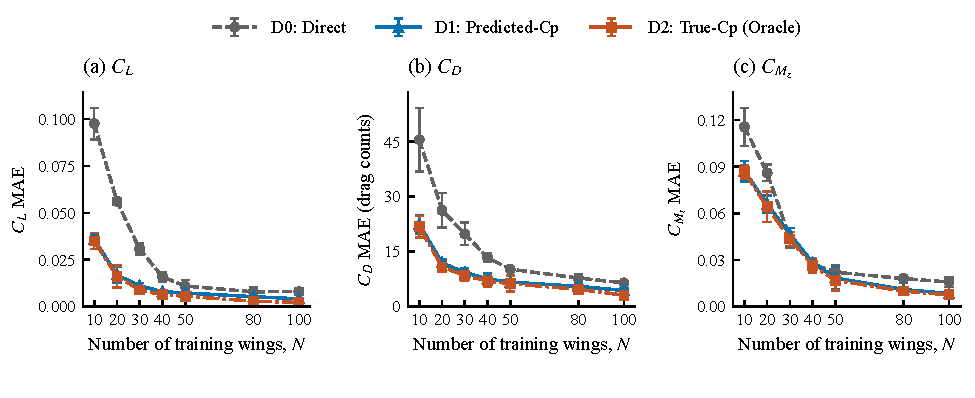
\includegraphics[width=0.96\textwidth]{V_Results_and_Discussion/figures/V_E_Fig25/V_E_Fig25_ve_force_mae.pdf}
    \caption{Force-coefficient MAE versus training size: (a) $C_L$, (b) $C_D$, and (c) $C_{M_z}$. D0, D1, and D2 use geometry/flow, M2-predicted pressure, and CFD pressure, respectively .}
    \label{fig:ve-force-mae}
\end{figure*}

The pressure-conditioned model provides its largest practical benefit at low force-label budgets. At $N=20$, the MAEs of D0 for $C_L$, $C_D$, and $C_{M_z}$ are 0.05610, 26.27 drag counts, and 0.08609, respectively. With M2-predicted pressure as additional input, D1 reduces these values to 0.01680, 11.88 drag counts, and 0.06592, corresponding to reductions of 70.1\%, 54.8\%, and 23.4\%. The improvement is strongest for lift, whose integrated response is directly related to the surface pressure loading. The reduction in drag-coefficient error is also substantial. By comparison, the smaller gain in pitching moment suggests a less favorable mapping from the available pressure representation to that particular integrated response; the present experiments do not isolate the physical origin of this difference.

Across the investigated budgets, the MAE generally decreases as more force-labeled wings become available, while the benefit of pressure conditioning remains coefficient-dependent. D1 outperforms D0 in mean MAE at all seven budgets for $C_L$ and $C_D$. For $C_{M_z}$, however, D1 is slightly less accurate at $N=30$ and 40: its MAEs are 0.04664 and 0.02833, compared with 0.04419 and 0.02746 for D0. At $N=100$, D1 reaches MAEs of 0.00414 for $C_L$, 4.39 drag counts for $C_D$, and 0.00838 for $C_{M_z}$. These results demonstrate that the contribution of the intermediate pressure field is not uniform across the three coefficients or training budgets.

The D2 results help distinguish the information supplied by pressure from the ability of the downstream regressor to use it. At $N=20$, replacing predicted pressure with CFD-reference pressure yields only modest additional reductions, to MAEs of 0.01611, 10.83 drag counts, and 0.06422 for $C_L$, $C_D$, and $C_{M_z}$, respectively. The separation becomes more apparent at $N=100$, where D2 achieves 0.00220, 3.12 drag counts, and 0.00755, compared with 0.00414, 4.39 drag counts, and 0.00838 for D1. Thus, additional pressure fidelity is more effectively reflected in the coefficient estimates when more force-labeled examples are available. This observation is consistent with a limitation imposed by downstream regression under very small training budgets, although the present comparison does not establish that explanation uniquely. Furthermore, D1 and D2 are fitted separately, so their difference cannot be attributed solely to M2 pressure error. Because D2 requires CFD-reference pressure as an input, it is a diagnostic reference rather than a deployable geometry-to-force surrogate.

The MAE over all 88 wings is complemented in Table~\ref{tab:ve-force-mae} by Best90 and Best80 MAE, which average the 80 and 71 lowest absolute errors, respectively, within each evaluated model. At $N=20$, D1 gives a drag MAE of 11.88 counts over all test wings, compared with Best90 and Best80 values of 8.98 and 7.30 counts. The corresponding D0 values are 26.27, 20.74, and 17.26 counts. Hence, the improvement from pressure conditioning is also evident over the lower-error majority of the test wings, rather than being restricted to changes in a few high-error cases. The gap between the full and trimmed means nevertheless indicates an uneven distribution of errors across wing configurations. Since the wings retained by the Best90 and Best80 definitions can differ between models, these statistics characterize error concentration and do not replace the full-set MAE.

\begin{table*}[!t]
    \centering
    \caption{Force-coefficient MAEs on 88 test wings, averaged over three training subsets.}
    \label{tab:ve-force-mae}
    \begingroup
    \fontsize{8.2}{9.8}\selectfont
    \setlength{\tabcolsep}{3.0pt}
    \renewcommand{\arraystretch}{1.06}

    \begin{tabular}{@{}r*{9}{c}@{}}
    \hline
    & \multicolumn{3}{c}{MAE}
    & \multicolumn{3}{c}{Best90 MAE}
    & \multicolumn{3}{c}{Best80 MAE} \\
    $N$ & D0 & D1 & D2
        & D0 & D1 & D2
        & D0 & D1 & D2 \\
    \hline

    \multicolumn{10}{@{}l}{\textit{$C_L$ (dimensionless)}} \\
    10  & 0.09764 & 0.03584 & 0.03501 & 0.08258 & 0.02785 & 0.02726 & 0.07027 & 0.02315 & 0.02260 \\
    20  & 0.05610 & 0.01680 & 0.01611 & 0.04473 & 0.01295 & 0.01211 & 0.03673 & 0.01055 & 0.00978 \\
    30  & 0.03067 & 0.01113 & 0.00889 & 0.02520 & 0.00903 & 0.00708 & 0.02082 & 0.00729 & 0.00568 \\
    40  & 0.01592 & 0.00791 & 0.00626 & 0.01263 & 0.00620 & 0.00484 & 0.01015 & 0.00511 & 0.00398 \\
    50  & 0.01095 & 0.00729 & 0.00557 & 0.00793 & 0.00563 & 0.00429 & 0.00647 & 0.00455 & 0.00346 \\
    80  & 0.00787 & 0.00529 & 0.00287 & 0.00558 & 0.00411 & 0.00218 & 0.00444 & 0.00347 & 0.00182 \\
    100 & 0.00800 & 0.00414 & 0.00220 & 0.00580 & 0.00335 & 0.00174 & 0.00478 & 0.00274 & 0.00145 \\

    \hline
    \multicolumn{10}{@{}l}{\textit{$C_D$ (drag counts)}} \\
    10  & 45.56 & 22.44 & 21.82 & 38.36 & 17.33 & 16.83 & 32.99 & 14.55 & 14.20 \\
    20  & 26.27 & 11.88 & 10.83 & 20.74 & 8.98 & 8.17 & 17.26 & 7.30 & 6.76 \\
    30  & 19.83 & 9.33 & 8.47 & 15.21 & 6.21 & 5.56 & 12.41 & 4.65 & 4.37 \\
    40  & 13.34 & 7.54 & 7.00 & 9.95 & 4.70 & 4.40 & 8.01 & 3.51 & 3.42 \\
    50  & 10.20 & 6.67 & 6.26 & 7.15 & 3.81 & 3.47 & 5.62 & 2.76 & 2.62 \\
    80  & 7.79 & 5.51 & 4.69 & 4.96 & 3.29 & 2.61 & 3.87 & 2.38 & 1.97 \\
    100 & 6.47 & 4.39 & 3.12 & 4.73 & 2.93 & 2.18 & 3.79 & 2.21 & 1.70 \\

    \hline
    \multicolumn{10}{@{}l}{\textit{$C_{M_z}$ (dimensionless)}} \\
    10  & 0.11566 & 0.08714 & 0.08674 & 0.09678 & 0.07124 & 0.07112 & 0.08294 & 0.05965 & 0.05956 \\
    20  & 0.08609 & 0.06592 & 0.06422 & 0.07016 & 0.05444 & 0.05251 & 0.06067 & 0.04643 & 0.04434 \\
    30  & 0.04419 & 0.04664 & 0.04351 & 0.03604 & 0.03874 & 0.03608 & 0.02976 & 0.03283 & 0.03051 \\
    40  & 0.02746 & 0.02833 & 0.02650 & 0.02139 & 0.02264 & 0.02140 & 0.01756 & 0.01881 & 0.01796 \\
    50  & 0.02210 & 0.01837 & 0.01695 & 0.01680 & 0.01481 & 0.01363 & 0.01394 & 0.01202 & 0.01136 \\
    80  & 0.01800 & 0.01098 & 0.00997 & 0.01326 & 0.00874 & 0.00826 & 0.01109 & 0.00735 & 0.00701 \\
    100 & 0.01574 & 0.00838 & 0.00755 & 0.01146 & 0.00681 & 0.00632 & 0.00984 & 0.00576 & 0.00537 \\

    \hline
    \end{tabular}
    \endgroup
\end{table*}

The representative small-sample case in Fig.~\ref{fig:ve-force-parity} provides a complementary view of the error distribution. At $N=20$, D1 predictions for lift and drag lie appreciably closer to the ideal agreement line than those of D0; the pitching-moment predictions remain more dispersed, consistent with their smaller relative MAE reduction. To prevent repeated evaluations of the same wing from appearing as independent observations, each plotted prediction is the arithmetic mean of the outputs from the three training-subset models for that wing. This averaging is used only for visualization: the metrics in Fig.~\ref{fig:ve-force-mae} and Table~\ref{tab:ve-force-mae} are calculated separately for each training subset before aggregation. Taken together, the results indicate that the fixed hierarchical pressure representation improves coefficient estimation when force labels are scarce, particularly for lift and drag, while leaving a coefficient-dependent residual error that is more apparent for challenging configurations.

\begin{figure*}[!t]
    \centering
    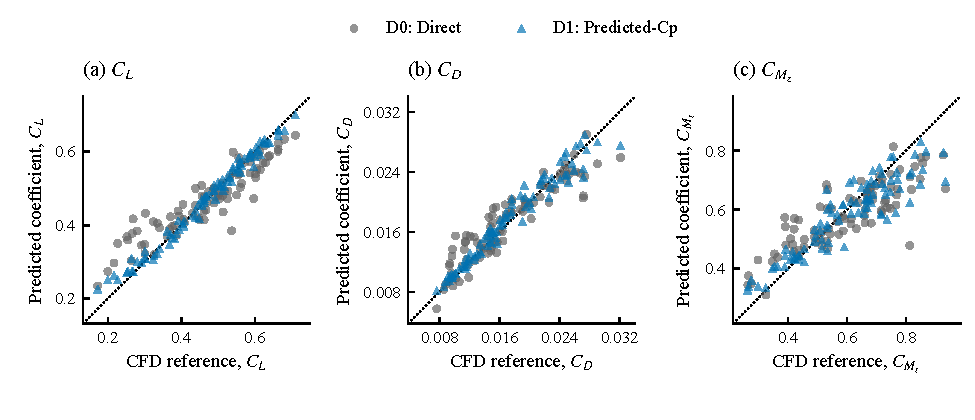
\includegraphics[width=0.96\textwidth]{V_Results_and_Discussion/figures/V_E_Fig26/V_E_Fig26_ve_force_parity.pdf}
    \caption{Predicted versus CFD-reference (a) lift, (b) drag, and (c) pitching-moment coefficients for D0 and D1 at $N=20$. Each point represents one of 88 test wings, with predictions averaged over three training subsets.}
    \label{fig:ve-force-parity}
\end{figure*}



\subsection{Aerodynamic Coefficient Prediction Performance}
\label{subsec:aerodynamic-coefficient-prediction}

Accurate reconstruction of the surface pressure field does not, by itself, guarantee accurate prediction of integrated aerodynamic coefficients. The latter requires a downstream model to extract the load-relevant information from a high-dimensional pressure representation. The force-label efficiency of this representation is examined using three coefficient-regression strategies: direct regression from geometry and flow conditions (D0), regression conditioned on the pressure field predicted by the fixed M2 model (D1), and regression conditioned on CFD-reference pressure (D2). Separate regressors are trained for the lift coefficient $C_L$, drag coefficient $C_D$, and pitching-moment coefficient $C_{M_z}$. Seven force-label budgets, $N=10$, 20, 30, 40, 50, 80, and 100 wings, are considered, with three independently sampled training subsets at each budget. All reported errors are evaluated on the same 88 test wings. Here $N$ denotes the number of wings used to train the downstream coefficient regressors; the pressure supervision previously used to establish the fixed M2 model is not included in this budget. Figure~\ref{fig:ve-force-mae} shows the mean absolute error (MAE) across the seven budgets, and Table~\ref{tab:ve-force-mae} provides the corresponding numerical comparisons.

\begin{figure*}[!t]
    \centering
    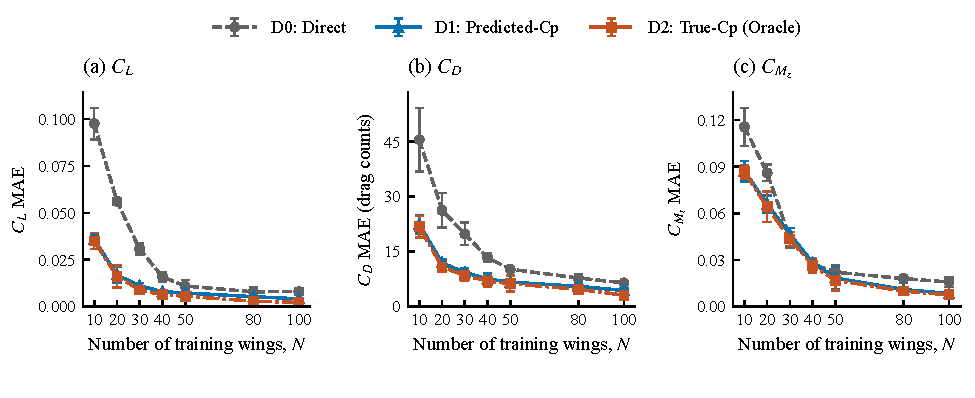
\includegraphics[width=0.96\textwidth]{V_Results_and_Discussion/figures/V_E_Fig25/V_E_Fig25_ve_force_mae.pdf}
    \caption{Force-coefficient MAE versus training size: (a) $C_L$, (b) $C_D$, and (c) $C_{M_z}$. D0, D1, and D2 use geometry/flow, M2-predicted pressure, and CFD pressure, respectively .}
    \label{fig:ve-force-mae}
\end{figure*}

The pressure-conditioned model provides its largest practical benefit at low force-label budgets. At $N=20$, the MAEs of D0 for $C_L$, $C_D$, and $C_{M_z}$ are 0.05610, 26.27 drag counts, and 0.08609, respectively. With M2-predicted pressure as additional input, D1 reduces these values to 0.01680, 11.88 drag counts, and 0.06592, corresponding to reductions of 70.1\%, 54.8\%, and 23.4\%. The improvement is strongest for lift, whose integrated response is directly related to the surface pressure loading. The reduction in drag-coefficient error is also substantial. By comparison, the smaller gain in pitching moment suggests a less favorable mapping from the available pressure representation to that particular integrated response; the present experiments do not isolate the physical origin of this difference.

Across the investigated budgets, the MAE generally decreases as more force-labeled wings become available, while the benefit of pressure conditioning remains coefficient-dependent. D1 outperforms D0 in mean MAE at all seven budgets for $C_L$ and $C_D$. For $C_{M_z}$, however, D1 is slightly less accurate at $N=30$ and 40: its MAEs are 0.04664 and 0.02833, compared with 0.04419 and 0.02746 for D0. At $N=100$, D1 reaches MAEs of 0.00414 for $C_L$, 4.39 drag counts for $C_D$, and 0.00838 for $C_{M_z}$. These results demonstrate that the contribution of the intermediate pressure field is not uniform across the three coefficients or training budgets.

The D2 results help distinguish the information supplied by pressure from the ability of the downstream regressor to use it. At $N=20$, replacing predicted pressure with CFD-reference pressure yields only modest additional reductions, to MAEs of 0.01611, 10.83 drag counts, and 0.06422 for $C_L$, $C_D$, and $C_{M_z}$, respectively. The separation becomes more apparent at $N=100$, where D2 achieves 0.00220, 3.12 drag counts, and 0.00755, compared with 0.00414, 4.39 drag counts, and 0.00838 for D1. Thus, additional pressure fidelity is more effectively reflected in the coefficient estimates when more force-labeled examples are available. This observation is consistent with a limitation imposed by downstream regression under very small training budgets, although the present comparison does not establish that explanation uniquely. Furthermore, D1 and D2 are fitted separately, so their difference cannot be attributed solely to M2 pressure error. Because D2 requires CFD-reference pressure as an input, it is a diagnostic reference rather than a deployable geometry-to-force surrogate.

The MAE over all 88 wings is complemented in Table~\ref{tab:ve-force-mae} by Best90 and Best80 MAE, which average the 80 and 71 lowest absolute errors, respectively, within each evaluated model. At $N=20$, D1 gives a drag MAE of 11.88 counts over all test wings, compared with Best90 and Best80 values of 8.98 and 7.30 counts. The corresponding D0 values are 26.27, 20.74, and 17.26 counts. Hence, the improvement from pressure conditioning is also evident over the lower-error majority of the test wings, rather than being restricted to changes in a few high-error cases. The gap between the full and trimmed means nevertheless indicates an uneven distribution of errors across wing configurations. Since the wings retained by the Best90 and Best80 definitions can differ between models, these statistics characterize error concentration and do not replace the full-set MAE.

\begin{table*}[!t]
    \centering
    \caption{Force-coefficient MAEs on 88 test wings, averaged over three training subsets.}
    \label{tab:ve-force-mae}
    \begingroup
    \fontsize{8.2}{9.8}\selectfont
    \setlength{\tabcolsep}{3.0pt}
    \renewcommand{\arraystretch}{1.06}

    \begin{tabular}{@{}r*{9}{c}@{}}
    \hline
    & \multicolumn{3}{c}{MAE}
    & \multicolumn{3}{c}{Best90 MAE}
    & \multicolumn{3}{c}{Best80 MAE} \\
    $N$ & D0 & D1 & D2
        & D0 & D1 & D2
        & D0 & D1 & D2 \\
    \hline

    \multicolumn{10}{@{}l}{\textit{$C_L$ (dimensionless)}} \\
    10  & 0.09764 & 0.03584 & 0.03501 & 0.08258 & 0.02785 & 0.02726 & 0.07027 & 0.02315 & 0.02260 \\
    20  & 0.05610 & 0.01680 & 0.01611 & 0.04473 & 0.01295 & 0.01211 & 0.03673 & 0.01055 & 0.00978 \\
    30  & 0.03067 & 0.01113 & 0.00889 & 0.02520 & 0.00903 & 0.00708 & 0.02082 & 0.00729 & 0.00568 \\
    40  & 0.01592 & 0.00791 & 0.00626 & 0.01263 & 0.00620 & 0.00484 & 0.01015 & 0.00511 & 0.00398 \\
    50  & 0.01095 & 0.00729 & 0.00557 & 0.00793 & 0.00563 & 0.00429 & 0.00647 & 0.00455 & 0.00346 \\
    80  & 0.00787 & 0.00529 & 0.00287 & 0.00558 & 0.00411 & 0.00218 & 0.00444 & 0.00347 & 0.00182 \\
    100 & 0.00800 & 0.00414 & 0.00220 & 0.00580 & 0.00335 & 0.00174 & 0.00478 & 0.00274 & 0.00145 \\

    \hline
    \multicolumn{10}{@{}l}{\textit{$C_D$ (drag counts)}} \\
    10  & 45.56 & 22.44 & 21.82 & 38.36 & 17.33 & 16.83 & 32.99 & 14.55 & 14.20 \\
    20  & 26.27 & 11.88 & 10.83 & 20.74 & 8.98 & 8.17 & 17.26 & 7.30 & 6.76 \\
    30  & 19.83 & 9.33 & 8.47 & 15.21 & 6.21 & 5.56 & 12.41 & 4.65 & 4.37 \\
    40  & 13.34 & 7.54 & 7.00 & 9.95 & 4.70 & 4.40 & 8.01 & 3.51 & 3.42 \\
    50  & 10.20 & 6.67 & 6.26 & 7.15 & 3.81 & 3.47 & 5.62 & 2.76 & 2.62 \\
    80  & 7.79 & 5.51 & 4.69 & 4.96 & 3.29 & 2.61 & 3.87 & 2.38 & 1.97 \\
    100 & 6.47 & 4.39 & 3.12 & 4.73 & 2.93 & 2.18 & 3.79 & 2.21 & 1.70 \\

    \hline
    \multicolumn{10}{@{}l}{\textit{$C_{M_z}$ (dimensionless)}} \\
    10  & 0.11566 & 0.08714 & 0.08674 & 0.09678 & 0.07124 & 0.07112 & 0.08294 & 0.05965 & 0.05956 \\
    20  & 0.08609 & 0.06592 & 0.06422 & 0.07016 & 0.05444 & 0.05251 & 0.06067 & 0.04643 & 0.04434 \\
    30  & 0.04419 & 0.04664 & 0.04351 & 0.03604 & 0.03874 & 0.03608 & 0.02976 & 0.03283 & 0.03051 \\
    40  & 0.02746 & 0.02833 & 0.02650 & 0.02139 & 0.02264 & 0.02140 & 0.01756 & 0.01881 & 0.01796 \\
    50  & 0.02210 & 0.01837 & 0.01695 & 0.01680 & 0.01481 & 0.01363 & 0.01394 & 0.01202 & 0.01136 \\
    80  & 0.01800 & 0.01098 & 0.00997 & 0.01326 & 0.00874 & 0.00826 & 0.01109 & 0.00735 & 0.00701 \\
    100 & 0.01574 & 0.00838 & 0.00755 & 0.01146 & 0.00681 & 0.00632 & 0.00984 & 0.00576 & 0.00537 \\

    \hline
    \end{tabular}
    \endgroup
\end{table*}

The representative small-sample case in Fig.~\ref{fig:ve-force-parity} provides a complementary view of the error distribution. At $N=20$, D1 predictions for lift and drag lie appreciably closer to the ideal agreement line than those of D0; the pitching-moment predictions remain more dispersed, consistent with their smaller relative MAE reduction. To prevent repeated evaluations of the same wing from appearing as independent observations, each plotted prediction is the arithmetic mean of the outputs from the three training-subset models for that wing. This averaging is used only for visualization: the metrics in Fig.~\ref{fig:ve-force-mae} and Table~\ref{tab:ve-force-mae} are calculated separately for each training subset before aggregation. Taken together, the results indicate that the fixed hierarchical pressure representation improves coefficient estimation when force labels are scarce, particularly for lift and drag, while leaving a coefficient-dependent residual error that is more apparent for challenging configurations.

\begin{figure*}[!t]
    \centering
    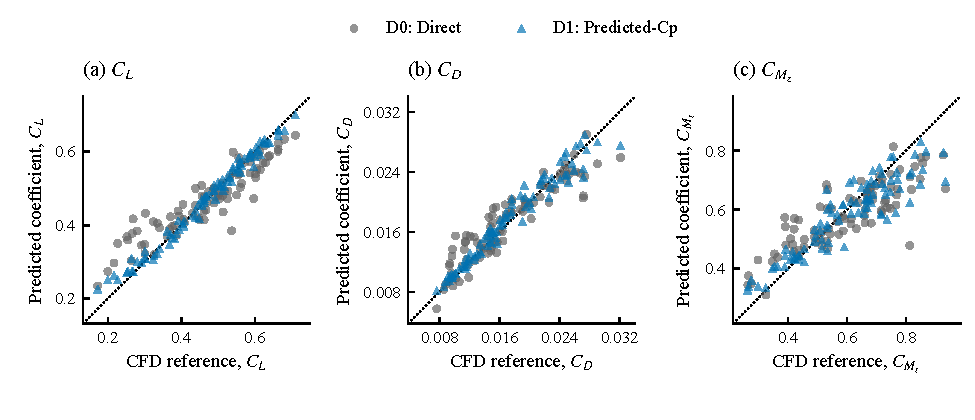
\includegraphics[width=0.96\textwidth]{V_Results_and_Discussion/figures/V_E_Fig26/V_E_Fig26_ve_force_parity.pdf}
    \caption{Predicted versus CFD-reference (a) lift, (b) drag, and (c) pitching-moment coefficients for D0 and D1 at $N=20$. Each point represents one of 88 test wings, with predictions averaged over three training subsets.}
    \label{fig:ve-force-parity}
\end{figure*}



\subsection{Aerodynamic Coefficient Prediction Performance}
\label{subsec:aerodynamic-coefficient-prediction}

Accurate reconstruction of the surface pressure field does not, by itself, guarantee accurate prediction of integrated aerodynamic coefficients. The latter requires a downstream model to extract the load-relevant information from a high-dimensional pressure representation. The force-label efficiency of this representation is examined using three coefficient-regression strategies: direct regression from geometry and flow conditions (D0), regression conditioned on the pressure field predicted by the fixed M2 model (D1), and regression conditioned on CFD-reference pressure (D2). Separate regressors are trained for the lift coefficient $C_L$, drag coefficient $C_D$, and pitching-moment coefficient $C_{M_z}$. Seven force-label budgets, $N=10$, 20, 30, 40, 50, 80, and 100 wings, are considered, with three independently sampled training subsets at each budget. All reported errors are evaluated on the same 88 test wings. Here $N$ denotes the number of wings used to train the downstream coefficient regressors; the pressure supervision previously used to establish the fixed M2 model is not included in this budget. Figure~\ref{fig:ve-force-mae} shows the mean absolute error (MAE) across the seven budgets, and Table~\ref{tab:ve-force-mae} provides the corresponding numerical comparisons.

\begin{figure*}[!t]
    \centering
    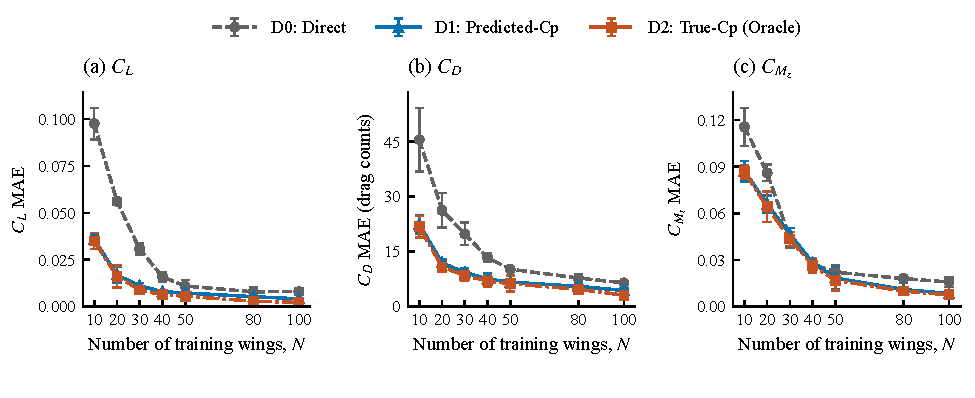
\includegraphics[width=0.96\textwidth]{V_Results_and_Discussion/figures/V_E_Fig25/V_E_Fig25_ve_force_mae.pdf}
    \caption{Force-coefficient MAE versus training size: (a) $C_L$, (b) $C_D$, and (c) $C_{M_z}$. D0, D1, and D2 use geometry/flow, M2-predicted pressure, and CFD pressure, respectively .}
    \label{fig:ve-force-mae}
\end{figure*}

The pressure-conditioned model provides its largest practical benefit at low force-label budgets. At $N=20$, the MAEs of D0 for $C_L$, $C_D$, and $C_{M_z}$ are 0.05610, 26.27 drag counts, and 0.08609, respectively. With M2-predicted pressure as additional input, D1 reduces these values to 0.01680, 11.88 drag counts, and 0.06592, corresponding to reductions of 70.1\%, 54.8\%, and 23.4\%. The improvement is strongest for lift, whose integrated response is directly related to the surface pressure loading. The reduction in drag-coefficient error is also substantial. By comparison, the smaller gain in pitching moment suggests a less favorable mapping from the available pressure representation to that particular integrated response; the present experiments do not isolate the physical origin of this difference.

Across the investigated budgets, the MAE generally decreases as more force-labeled wings become available, while the benefit of pressure conditioning remains coefficient-dependent. D1 outperforms D0 in mean MAE at all seven budgets for $C_L$ and $C_D$. For $C_{M_z}$, however, D1 is slightly less accurate at $N=30$ and 40: its MAEs are 0.04664 and 0.02833, compared with 0.04419 and 0.02746 for D0. At $N=100$, D1 reaches MAEs of 0.00414 for $C_L$, 4.39 drag counts for $C_D$, and 0.00838 for $C_{M_z}$. These results demonstrate that the contribution of the intermediate pressure field is not uniform across the three coefficients or training budgets.

The D2 results help distinguish the information supplied by pressure from the ability of the downstream regressor to use it. At $N=20$, replacing predicted pressure with CFD-reference pressure yields only modest additional reductions, to MAEs of 0.01611, 10.83 drag counts, and 0.06422 for $C_L$, $C_D$, and $C_{M_z}$, respectively. The separation becomes more apparent at $N=100$, where D2 achieves 0.00220, 3.12 drag counts, and 0.00755, compared with 0.00414, 4.39 drag counts, and 0.00838 for D1. Thus, additional pressure fidelity is more effectively reflected in the coefficient estimates when more force-labeled examples are available. This observation is consistent with a limitation imposed by downstream regression under very small training budgets, although the present comparison does not establish that explanation uniquely. Furthermore, D1 and D2 are fitted separately, so their difference cannot be attributed solely to M2 pressure error. Because D2 requires CFD-reference pressure as an input, it is a diagnostic reference rather than a deployable geometry-to-force surrogate.

The MAE over all 88 wings is complemented in Table~\ref{tab:ve-force-mae} by Best90 and Best80 MAE, which average the 80 and 71 lowest absolute errors, respectively, within each evaluated model. At $N=20$, D1 gives a drag MAE of 11.88 counts over all test wings, compared with Best90 and Best80 values of 8.98 and 7.30 counts. The corresponding D0 values are 26.27, 20.74, and 17.26 counts. Hence, the improvement from pressure conditioning is also evident over the lower-error majority of the test wings, rather than being restricted to changes in a few high-error cases. The gap between the full and trimmed means nevertheless indicates an uneven distribution of errors across wing configurations. Since the wings retained by the Best90 and Best80 definitions can differ between models, these statistics characterize error concentration and do not replace the full-set MAE.

\begin{table*}[!t]
    \centering
    \caption{Force-coefficient MAEs on 88 test wings, averaged over three training subsets.}
    \label{tab:ve-force-mae}
    \begingroup
    \fontsize{8.2}{9.8}\selectfont
    \setlength{\tabcolsep}{3.0pt}
    \renewcommand{\arraystretch}{1.06}

    \begin{tabular}{@{}r*{9}{c}@{}}
    \hline
    & \multicolumn{3}{c}{MAE}
    & \multicolumn{3}{c}{Best90 MAE}
    & \multicolumn{3}{c}{Best80 MAE} \\
    $N$ & D0 & D1 & D2
        & D0 & D1 & D2
        & D0 & D1 & D2 \\
    \hline

    \multicolumn{10}{@{}l}{\textit{$C_L$ (dimensionless)}} \\
    10  & 0.09764 & 0.03584 & 0.03501 & 0.08258 & 0.02785 & 0.02726 & 0.07027 & 0.02315 & 0.02260 \\
    20  & 0.05610 & 0.01680 & 0.01611 & 0.04473 & 0.01295 & 0.01211 & 0.03673 & 0.01055 & 0.00978 \\
    30  & 0.03067 & 0.01113 & 0.00889 & 0.02520 & 0.00903 & 0.00708 & 0.02082 & 0.00729 & 0.00568 \\
    40  & 0.01592 & 0.00791 & 0.00626 & 0.01263 & 0.00620 & 0.00484 & 0.01015 & 0.00511 & 0.00398 \\
    50  & 0.01095 & 0.00729 & 0.00557 & 0.00793 & 0.00563 & 0.00429 & 0.00647 & 0.00455 & 0.00346 \\
    80  & 0.00787 & 0.00529 & 0.00287 & 0.00558 & 0.00411 & 0.00218 & 0.00444 & 0.00347 & 0.00182 \\
    100 & 0.00800 & 0.00414 & 0.00220 & 0.00580 & 0.00335 & 0.00174 & 0.00478 & 0.00274 & 0.00145 \\

    \hline
    \multicolumn{10}{@{}l}{\textit{$C_D$ (drag counts)}} \\
    10  & 45.56 & 22.44 & 21.82 & 38.36 & 17.33 & 16.83 & 32.99 & 14.55 & 14.20 \\
    20  & 26.27 & 11.88 & 10.83 & 20.74 & 8.98 & 8.17 & 17.26 & 7.30 & 6.76 \\
    30  & 19.83 & 9.33 & 8.47 & 15.21 & 6.21 & 5.56 & 12.41 & 4.65 & 4.37 \\
    40  & 13.34 & 7.54 & 7.00 & 9.95 & 4.70 & 4.40 & 8.01 & 3.51 & 3.42 \\
    50  & 10.20 & 6.67 & 6.26 & 7.15 & 3.81 & 3.47 & 5.62 & 2.76 & 2.62 \\
    80  & 7.79 & 5.51 & 4.69 & 4.96 & 3.29 & 2.61 & 3.87 & 2.38 & 1.97 \\
    100 & 6.47 & 4.39 & 3.12 & 4.73 & 2.93 & 2.18 & 3.79 & 2.21 & 1.70 \\

    \hline
    \multicolumn{10}{@{}l}{\textit{$C_{M_z}$ (dimensionless)}} \\
    10  & 0.11566 & 0.08714 & 0.08674 & 0.09678 & 0.07124 & 0.07112 & 0.08294 & 0.05965 & 0.05956 \\
    20  & 0.08609 & 0.06592 & 0.06422 & 0.07016 & 0.05444 & 0.05251 & 0.06067 & 0.04643 & 0.04434 \\
    30  & 0.04419 & 0.04664 & 0.04351 & 0.03604 & 0.03874 & 0.03608 & 0.02976 & 0.03283 & 0.03051 \\
    40  & 0.02746 & 0.02833 & 0.02650 & 0.02139 & 0.02264 & 0.02140 & 0.01756 & 0.01881 & 0.01796 \\
    50  & 0.02210 & 0.01837 & 0.01695 & 0.01680 & 0.01481 & 0.01363 & 0.01394 & 0.01202 & 0.01136 \\
    80  & 0.01800 & 0.01098 & 0.00997 & 0.01326 & 0.00874 & 0.00826 & 0.01109 & 0.00735 & 0.00701 \\
    100 & 0.01574 & 0.00838 & 0.00755 & 0.01146 & 0.00681 & 0.00632 & 0.00984 & 0.00576 & 0.00537 \\

    \hline
    \end{tabular}
    \endgroup
\end{table*}

The representative small-sample case in Fig.~\ref{fig:ve-force-parity} provides a complementary view of the error distribution. At $N=20$, D1 predictions for lift and drag lie appreciably closer to the ideal agreement line than those of D0; the pitching-moment predictions remain more dispersed, consistent with their smaller relative MAE reduction. To prevent repeated evaluations of the same wing from appearing as independent observations, each plotted prediction is the arithmetic mean of the outputs from the three training-subset models for that wing. This averaging is used only for visualization: the metrics in Fig.~\ref{fig:ve-force-mae} and Table~\ref{tab:ve-force-mae} are calculated separately for each training subset before aggregation. Taken together, the results indicate that the fixed hierarchical pressure representation improves coefficient estimation when force labels are scarce, particularly for lift and drag, while leaving a coefficient-dependent residual error that is more apparent for challenging configurations.

\begin{figure*}[!t]
    \centering
    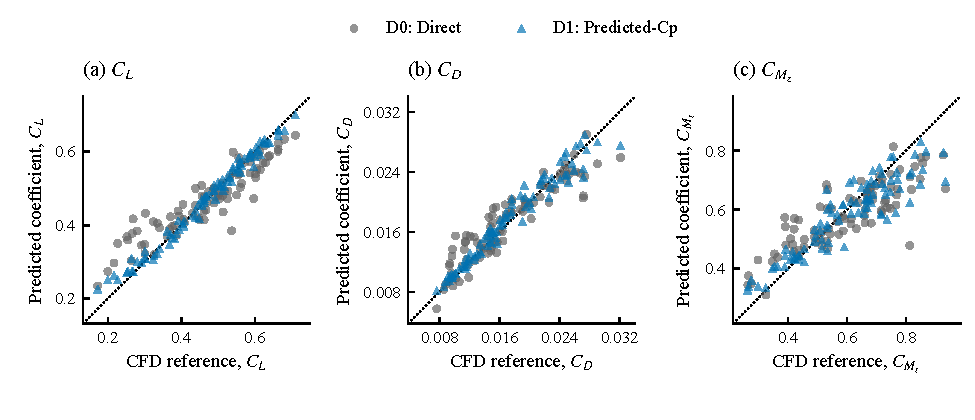
\includegraphics[width=0.96\textwidth]{V_Results_and_Discussion/figures/V_E_Fig26/V_E_Fig26_ve_force_parity.pdf}
    \caption{Predicted versus CFD-reference (a) lift, (b) drag, and (c) pitching-moment coefficients for D0 and D1 at $N=20$. Each point represents one of 88 test wings, with predictions averaged over three training subsets.}
    \label{fig:ve-force-parity}
\end{figure*}




\FloatBarrier

\section{Conclusions}
\label{sec:conclusions}

This study developed a hierarchical aerodynamic knowledge-transfer framework for data-efficient prediction of three-dimensional surface-pressure distributions on transonic swept wings. Reusable sectional pressure knowledge learned from infinite-span swept-wing data and localized wing-root and wing-tip corrections derived from paired finite- and infinite-span CFD data were mapped to the target configuration to construct a hierarchical pressure prior. A target-domain residual model was then trained using limited high-fidelity CFD samples to learn the remaining pressure discrepancy.

The results demonstrate the effectiveness of hierarchical knowledge transfer for data-efficient three-dimensional pressure prediction. With only 10 target-domain training wings, M2 reduced the surface-pressure RMSE by 65.74\% relative to the direct-learning baseline M0 and maintained the lowest mean prediction error across all investigated training budgets. Regional ablation results further demonstrate the complementary contributions of the root and tip knowledge models. At $N=20$, M2 reduced the mean RMSE relative to M1 by 39.81\%, 24.69\%, and 20.66\% in the root, midspan, and tip regions, respectively. These improvements indicate that regional knowledge provides benefits beyond the immediate vicinity of the corresponding spanwise boundaries, although the magnitude of improvement varies with spanwise position and surface.

The predicted pressure distributions also provide useful information for downstream aerodynamic-coefficient regression under limited force-label supervision. With 20 force-labeled target wings, D1, which uses pressure predictions from the fixed M2 model, reduced the mean absolute errors in lift, drag, and pitching-moment coefficients by 70.1\%, 54.8\%, and 23.4\%, respectively, relative to direct regression D0. The improvements were more pronounced for lift and drag than for pitching moment, indicating that the predictive benefit of pressure information depends on the aerodynamic quantity being modeled.

The principal contribution of this work lies in developing a hierarchical representation and transfer strategy that separates the reusable sectional aerodynamic response from localized three-dimensional pressure corrections. These complementary knowledge components are mapped and combined to construct a pressure prior for the target wing. This formulation shifts target-domain learning from directly fitting the entire three-dimensional pressure field to correcting the pressure variations not adequately captured by the transferred knowledge. Consequently, limited target-domain CFD samples can be more effectively utilized to learn configuration-dependent three-dimensional pressure characteristics rather than repeatedly learning the sectional responses already represented by the prior. This approach provides a basis for exploiting hierarchical aerodynamic knowledge in small-sample wing pressure prediction and for further integrating distributed pressure information into aerodynamic performance modeling.



\section*{Acknowledgments}


\bibliography{references}


\end{document}